% AEJ-Article.tex for AEA last revised 22 June 2011
\documentclass[AER]{AEA_mal}

% The mathtime package uses a Times font instead of Computer Modern.
% Uncomment the line below if you wish to use the mathtime package:
%\usepackage[cmbold]{mathtime}
% Note that miktex, by default, configures the mathtime package to use commercial fonts
% which you may not have. If you would like to use mathtime but you are seeing error
% messages about missing fonts (mtex.pfb, mtsy.pfb, or rmtmi.pfb) then please see
% the technical support document at http://www.aeaweb.org/templates/technical_support.pdf
% for instructions on fixing this problem.

% Note: you may use either harvard or natbib (but not both) to provide a wider
% variety of citation commands than latex supports natively. See below.

% Uncomment the next line to use the natbib package with bibtex
\usepackage[hyphens]{url}
\usepackage[utf8]{inputenc}
\usepackage[multiple]{footmisc}
\usepackage{bbm, graphicx, microtype, multirow, natbib, subcaption, tabularx, xcolor}

% Uncomment the next line to use the harvard package with bibtex
%\usepackage[abbr]{harvard}

% This command determines the leading (vertical space between lines) in draft mode
% with 1.5 corresponding to "double" spacing.
\draftSpacing{1.5}

\begin{document}

\title{Less is More Expensive: Income Differences in Bulk Buying}
\shortTitle{Income Differences in Bulk Buying}
\author{Mallick Hossain\thanks{%
Federal Reserve Bank of Philadelphia, Ten Independence Mall, Philadelphia, PA, 19106, mallick.hossain@phil.frb.org. The views expressed here are those of the author and do not necessarily represent the views of the Federal Reserve Bank of Philadelphia or the Federal Reserve System. This article is based on a chapter of my dissertation. I thank my advisers, Katja Seim, Holger Sieg, Aviv Nevo, and Sarah Moshary for their advice and constructive criticism. Thanks to Mike Abito, Francesco Agostinelli, Emek Basker, Minsu Chang, Chris Cronin, Frank DiTraglia, Eileen Divringi, Hanming Fang, Jim Ferry, Ishan Ghosh, Joao Granja, Kathleen Hui, Ben Hyman, Jeff Lin, Paolo Martellini, Davin Reed, Claudia Sahm, Paul Sangrey, Andrew Shephard, Petra Todd, Anna Tranfaglia, and Keith Wardrip for their comments. Thanks to Dmitri Koustas for providing data on warehouse clubs. The conclusions drawn from the Nielsen data are those of the researcher and do not reflect the views of Nielsen. Nielsen is not responsible for, had no role in, and was not involved in analyzing and preparing the results reported herein.}}
\date{\today}
% \pubMonth{Month}
% \pubYear{Year}
% \pubVolume{Vol}
% \pubIssue{Issue}
\JEL{}
\Keywords{}

\begin{abstract}
\noindent Quantity discounts are an effective way for households to save money. I explore how large these quantity discounts are, how bulk buying differs by income, and how other factors affect the bulk buying decision. Using Nielsen's granular store- and household-level data, I establish two empirical facts. First, quantity discounts are large for a wide range of products. Second, low-income households are less likely to buy in bulk than high-income households. I estimate that low-income households could reduce their grocery expenditures by 5\%, saving an aggregate of \$5.4 billion annually, if they bought in bulk to the same extent as high-income households. I augment Nielsen data with new data that I collect on state-level unit-price regulations and on warehouse club entry. I find that a combination of cognitive costs, store preferences, budget constraints, and storage costs discourage low-income households from realizing these savings. I then estimate a discrete choice model of household purchasing behavior to quantify how bulk buying changes when cognitive costs and storage costs are reduced. Counterfactual simulations show that mandating the display of unit prices, which has only been adopted by nine states, would reduce the difference in how often the highest- and lowest-income households buy in bulk by 26\%.
\end{abstract}

\maketitle

\newpage

\section{Introduction}
Grocery purchases account for a sizable share of a household's discretionary spending, especially for the lowest-income households \citep{bls2017}. To save money, households often wait for sales, redeem coupons, or purchase generic brands \citep{nevo2009}. Low-income households also increase their home production to reduce their spending \citep{aguiar2005}. Quantity discounts are another way for households to save money. Even though households buy more on a given shopping trip, they pay lower unit prices, and reduce their overall spending.

I examine how large these quantity discounts are, how bulk buying varies by income groups, and which factors influence the decision to buy in bulk. Most explanations for why households pay different prices for the same product relate to differences in search behavior. Prices vary based on where households shop or whether they use coupons \citep{talukdar2008,nevo2009}. However, even in the absence of sales and coupons, prices for the same product often differ within a store due to quantity discounts.

This paper contributes new findings that, despite the substantial savings available from quantity discounts, low-income households are less likely to buy in bulk than high-income households.\footnote{Throughout this paper, ``high-income'' refers to households making over \$100,000 and ``low-income'' refers to households making under \$25,000.} \citet{kunreuther1973} provides the first evidence of this ``bulk buying gap'' for a few specific products and \citet{orhun2018} expands this finding to a whole product category. Since households purchase a variety of products when shopping, I show that the bulk buying gap exists across the full range of product categories that households purchase.

I find that cognitive costs, store preferences, budget constraints, and storage costs all contribute to this bulk buying gap. First, the cognitive costs of assessing price differences across products can prevent households from making economical decisions \citep{mitchell2003}. Providing price information reduces the effort needed to compare prices, and households change their purchase decisions when such information is  prominently displayed \citep{chetty2009, bogomolova2016}. Posting unit prices reduces the cognitive costs of comparing unit prices across different products. Sixteen states have regulations governing the display of unit prices, but no study has evaluated the impact of these regulations on consumer behavior. I provide the first nationwide study of the impact of displaying unit prices on bulk purchasing and find that households are significantly more likely to buy in bulk when retailers are mandated to display unit prices.

Second, households may make different purchase decisions based on where they live or where they shop \citep{chung1999, talukdar2008, handbury2019}. I show that even within neighborhoods, there are large differences in bulk buying between high- and low-income households. Even after controlling for where households shop, income differences in bulk buying persist.

Third, budget constraints affect bulk buying because low-income households may not have enough cash on hand to purchase a bulk package. Leveraging within-month variation in budgets, I show that the lowest-income households slightly decrease their bulk purchasing towards the end of month, presumably when their budget constraint is binding. In contrast, middle- and high-income households either do not change their bulk buying or slightly increase their bulk buying towards the end of the month.

Fourth, storage costs also affect the bulk buying decision because even though large packages provide lower unit prices, they are more cumbersome to store. I show that households are more likely to buy in bulk when they live in larger homes and when products are smaller. I provide a new approach to estimate storage costs cross-sectionally using differences in product ``concentration.'' One way of identifying household-level storage costs compares purchase frequencies of households with the same demand for a product \citep{hendel2006a}. A household with high storage costs will purchase small packages more frequently. I propose a complementary approach: I compare purchases of products that are otherwise identical, but differ in their level of concentration. All else equal, households who buy smaller, more concentrated packages have higher storage costs than those that buy larger, less concentrated packages. Based on this approach, I find that low-income households have higher storage costs than high-income households. On balance, this means that firms extract higher rents from low-income households because they have less ability to store for future consumption.

For my analysis, I combine household- and store-level datasets to study income heterogeneity in bulk buying. Nielsen's Consumer Panel data are a nationally representative panel survey of household grocery purchases, and Nielsen's Retail Scanner data are a national panel of weekly UPC-level sales data from over 30,000 stores. I construct a new dataset of state-level per-unit pricing regulations, including a measure of regulatory stringency. I also use data on entry dates and locations of over 1,400 warehouse clubs in the United States. As a result, I have a comprehensive view of a household's possible product choices, available price information, retail environment, and resulting expenditures.

I find that low-income households could realize substantial savings from buying in bulk at the same rate as high-income households. To do this, I estimate the average bulk discount for each product category based on Nielsen's weekly store-level price and product data. The average discount across all product categories is such that a 10\% larger package has a 5\% lower unit price. Then, I estimate how much each household buys in bulk using Nielsen's household-level purchase data. Given each product category-specific bulk discount and household-level bulk buying, I predict how much low-income households could save if they increased their bulk buying intensity to match that of high-income households. I find that low-income households would reduce their annual grocery expenditures by 5\% if they bought in bulk like high-income households, saving an aggregate of \$5.4 billion annually.

I then employ three differences-in-differences models to determine how much cognitive costs, store preferences, and budget constraints affect bulk buying. The first model uses a novel dataset that I compiled of state regulations regarding the display of per-unit prices and exploits the fact that a significant share of households in the Nielsen Consumer Panel moves between regulatory regimes when they move from one state to another. Before households move to a state without unit price posting requirements, their bulk buying behavior is similar to that of households that remain in the same regulatory regime. After households move, however, I find that their bulk buying is 4--5\% lower than that of households who did not experience a regulatory change.

The second differences-in-differences model shows how much store preferences, particularly for warehouse clubs, affect bulk buying. The bulk buying gap narrows substantially after controlling for the types of stores households shop at; high-income households spend a larger portion of their budget at warehouse clubs. To estimate the effect of warehouse clubs on bulk buying, I examine how bulk buying changes within households before and after a warehouse club enters nearby. Before a warehouse club enters, bulk buying is similar for households that will and will not experience a warehouse club entry. After a warehouse club enters, however, I find bulk buying increases by 5--10\% compared to households that did not experience an entry within a 15-mile radius. This increase is only limited to middle- and high-income households and is due to increased shopping at warehouse clubs.

The third differences-in-differences model analyzes how budget constraints affect bulk buying. To do this, I analyze within-household changes in bulk buying over the course of a month because the liquidity of poorer households decreases towards the end of the month \citep{orhun2018}. Using information on weekly bulk buying from Nielsen, I find that low-income households slightly decrease their bulk buying by 0.5--1\% between the first half and second half of the month while middle- and high-income households slightly increase their bulk buying by 0.5--1.5\% over the same period.

I also assess the importance of storage costs using differences in bulk buying relative to the size of a household's home and relative to the physical size of the product being purchased. I examine how a household's bulk buying changes when it moves to a different type of housing, after controlling for other within-household changes. Bulk buying is 3--4\% higher for the same household when it lives in a single-family home relative to when it lives in an apartment, controlling for demographic differences between households. I also find that the bulk buying gap is smaller for products with smaller physical footprints.

Finally, I construct a discrete-choice model of consumer purchasing behavior to quantify consumer preferences and disentangle the contributions of cognitive and storage costs to the bulk buying decision. I estimate this model using data on toilet paper purchases. Households choose a product based on price, quantity, quality, and package size, which serves as a proxy for storage costs. I can separate preferences for quantity from size preferences because I demonstrate that toilet paper comes in varying ``concentrations.'' I allow state-level unit pricing mandates to affect a household’s unit price sensitivity. From this demand model, I simulate household responses to two counterfactuals: 1) universally posting unit prices and 2) reducing storage costs.

My model predicts that requiring stores to post unit prices would reduce the bulk buying gap in package size purchased between high- and low-income households by 26\%. Reducing storage costs would close the remainder of the gap and low-income households would actually buy more in bulk than high-income households. As a result of these policies, households would buy larger quantities of toilet paper and pay lower unit prices. Universally displaying unit prices would encourage households to better utilize quantity discounts by reducing cognitive costs, increasing bulk buying, and helping consumers save money.

The rest of the paper is structured as follows. Section \ref{data} describes the data. Section \ref{stylized} documents new facts of quantity discounting. Section \ref{factors} presents evidence of contributing factors to the bulk-buying gap. Section \ref{model} introduces the model. Section \ref{estimation} presents estimation and counterfactual results. Section \ref{conclusion} concludes.

\section{Data}
\label{data}
% source("../1_getData/getCensusData.R")
% source("../1_getData/getHomescan.R")
% source("../1_getData/getZIPIncomePop.R")
In this section, I describe the datasets used for my analysis and give a brief overview of their respective features.\footnote{Researcher's own analyses derived based in part on data from The Nielsen Company (US), LLC and marketing databases provided through the Nielsen Datasets at the Kilts Center for Marketing Data Center at The University of Chicago Booth School of Business.} Nielsen's Consumer Panel data provide information on households' shopping and purchasing decisions. Nielsen's Retail Scanner data provide information on weekly product assortments and prices. A new regulatory dataset I construct contains information on state-level regulations regarding the display of per-unit pricing. Finally, warehouse club data provide information on the location and entry dates of warehouse clubs across the United States. By combining these data, I have a comprehensive view into a household's possible product choices, available price information, retail environment, and their resulting purchase decision.

\subsection{Nielsen Consumer Panel Data}
% source("../4_analyzeData/wrds/homescanSummaryStats.R")

I use the Nielsen Consumer Panel dataset from 2004--2017. This dataset is a panel of about 178,000 unique households. I observe about 40,000 households each year from 2004--2006 and about 60,000 households each year from 2007--2017. Households scan all items that they purchase and then input information about quantities, prices, date of purchase, and store. Nielsen retains about 80\% of its panel from year to year with the mean and median tenure of a household being four and three years, respectively.

I consider food, drink, and non-food grocery (e.g., paper towels, toilet paper, detergent) purchases made at grocery stores, discount stores, dollar stores, warehouse clubs, and drug stores. These outlets account for over 90\% of household expenditures in these categories. I exclude alcohol, tobacco, health, and general merchandise products from my analysis since these products (e.g., cigarettes, painkillers) may have different consumption patterns than grocery products or are not suited for bulk purchases (e.g., printers, cookware, linens). I also exclude households with a student or military head of household as well as those with an annual income of less than \$5,000 and those living in mobile homes. Only about 7\% of households are excluded and I use the remaining 166,000 households for my analysis. See Appendix \ref{sec:sampleConstruction} for further details of sample construction.

Nielsen computes projection weights to ensure their sample is nationally representative. Weights are calculated to match population moments based on household size, income, age, race, ethnicity, education, occupation, and presence of children. All analyses use these projection weights unless otherwise stated. Nielsen groups household income into 16 different income bins. Due to the large number of bins, in tables and parts of the text, I will report differences by income quartiles. However, where possible (especially in graphs), I will report estimates for each income bin. Table \ref{tab:homescanSummaryStats} presents descriptive statistics for households in the sample.

\begin{table}[!htbp] \centering
\caption{Nielsen Consumer Panel Summary Statistics}
\label{tab:homescanSummaryStats}
\begin{tabular}{lcccc}
\\[-1.8ex]\hline
\hline \\[-1.8ex]
Variable                  & Mean  & SD    & 25th Pctile & 75th Pctile\\
\hline
Household income (\$000s) & 57.13 & 31.17 & 27.5        & 85 \\
Household size            & 2.56  & 1.45  & 1           & 3 \\
Age                       & 52.59 & 14.39 & 41.5        & 63 \\
College educated          & 0.39  & 0.49  & 0           & 1 \\
Child present             & 0.33  & 0.47  & 0           & 1 \\
Married                   & 0.50  & 0.50  & 0           & 1 \\
\hline
N (Household-Years)       & \multicolumn{4}{c}{734,724} \\
N (Households)            & \multicolumn{4}{c}{166,163} \\
\\[-1.8ex]\hline
\hline \\[-1.8ex]
\end{tabular}
\begin{tablenotes}
Household income is grouped into bins. Midpoints of each bin are used in order to calculated sample moments. Data are weighted for national representativeness.
\end{tablenotes}
\begin{tablenotes}[Source]
Nielsen Consumer Panel (2004--2017)
\end{tablenotes}
\end{table}


\subsection{Nielsen Scanner Data}
The Nielsen Scanner data contain average weekly prices and volume sold of individual products at about 35,000 stores from about 90 retail chains between 2006--2016. Average prices are weighted by the volume sold. Only products with positive sales in a given week are recorded. I match the Retail Scanner data with the Consumer Panel data based on store identification numbers and purchase dates. By matching the two datasets, I recover the set of products available to a household and the product it chose to purchase.

\subsection{Unit Pricing Regulations}
I compile a novel dataset on state-level regulations regarding the display of unit prices. The data are based on annual regulatory updates aggregated in Handbook 130 published by the National Institute of Standards and Technology \citep{nist130}. I cross-check this information with state regulatory codes and state officials to ensure accuracy. This data include information on which states have regulations, when they were adopted, and how stringent these regulations are. More details are discussed in Section \ref{salience}.

\subsection{Warehouse Club Data}
I also use data on all warehouse clubs in the United States between 2004--2015 gathered by \citet{coibion2017}. This data record information on the opening dates, locations, and identity of all warehouse clubs in the United States. It was gathered by combining information available on company websites, annual reports, and by contacting firms.

\section{Stylized Facts}
\label{stylized}

In this section, I document two new facts about quantity discounts. First, I show that quantity discounts apply to 91\% of grocery categories. Second, I document that households making over \$100,000 are 26\% more likely to buy non-food items in bulk than households making \$5,000--\$8,000 annually, compared to only 3\% for food items. Combining these findings, I estimate that low-income households could reduce their grocery expenditures by 5\%, saving an aggregate of \$5.4 billion annually, simply by buying in bulk at the same rate as high-income households.

\subsection{Quantity Discount Prevalence}
\label{prevalence}
%  This uses the bulkDiscount2016Scanner.R script
%  This uses the couponAndBulkSavings.R script
Quantity discounts are a specific form of non-linear pricing in which unit prices decrease as package size increases. To establish the prevalence and magnitude of quantity discounts, I use Nielsen's Retail Scanner data from 2016. I estimate quantity discounts using the following regression for each of the 693 product categories:\footnote{48 categories could not be estimated typically because the data did not have sufficient variation. These were generally uncommon categories like mushroom sauce, canned grapes, and canned chow mein.}
\begin{equation}
\label{eq:bulkDiscount}
\ln(P)_{ibm} = \alpha + \beta \ln(Size)_{ibm} + \lambda_{bm} + \epsilon_{ibm},
\end{equation}
where $P_{ibm}$ is the unit price (package price divided by package size) of product $i$ from brand $b$ purchased in market $m$ (defined as a store-week). $Size_{ibm}$ is the item's package size, which is the number of units included in a UPC (e.g., quart, square feet, count, pound). $\lambda_{bm}$ is a brand-store-week fixed effect. Variation in unit prices across package sizes within the same brand-store-week identify $\beta$.\footnote{Some readers may be concerned that the positive sales threshold limits the number of weeks products are observed. I find that a large majority of products (at the UPC level) are observed for over half of the year. The unobserved weeks can be attributed to a variety of reasons including zero sales, discontinued products, or missing reports from retailers. Observing products for most weeks of the year limits the possibility that quantity discounts are estimated on a limited subset of weeks.} If retailers offer quantity discounts, then $\beta$ will be negative.

Figure \ref{fig:bulkDiscountAllProds} plots the distribution of $\beta$ across product categories (statistically insignificant betas are zero). 91\% of all product categories have a statistically significant and negative $\beta$ and non-food items generally have larger discounts than food items.\footnote{Some products do have a significantly positive coefficient, indicating that unit prices increase with package size. These quantity ``surcharges'' are less common, but have been highlighted before \citep{sprott2003}.} The median $\beta$ is -0.51 for non-food products, which means that a 10\% increase in package size is associated with a 5.1\% decrease in unit price. This discount is larger than the median $\beta$ for food items (-0.43).\footnote{These findings are robust to outliers. Winsorizing unit prices at the 98th and 90th percentile produces almost identical estimates.} The size and near-universality of quantity discounts suggest they offer substantial savings to households without sacrificing consumption.\footnote{For a comparison of quantity discounts with coupons, see Appendix \ref{coupons}.}

\begin{figure}[!htb]
 \centering
 \caption{Distribution of Bulk Discounts by Product Type}
 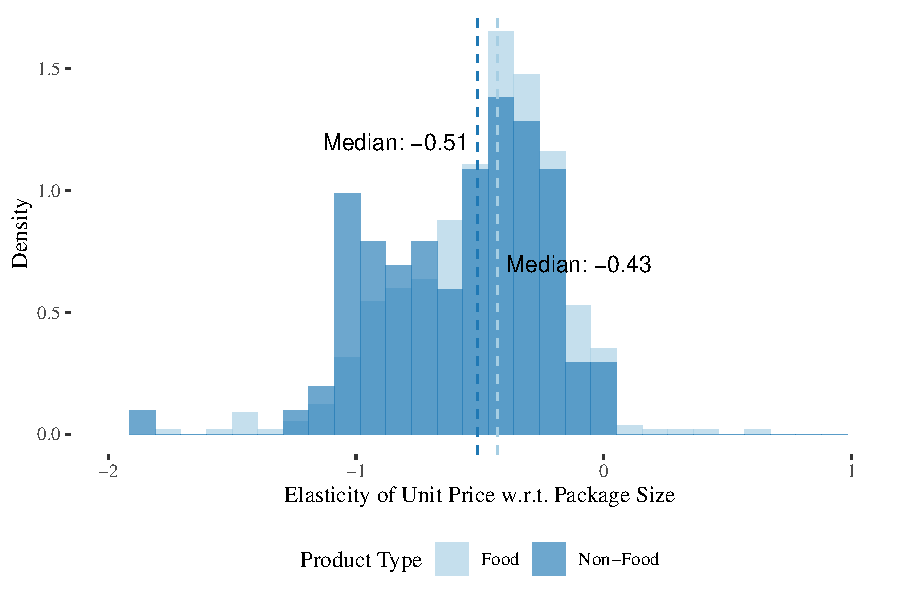
\includegraphics[width = 5in, height = 3in]{../5_figures/bulkDiscountAllProdsScanner.pdf}
 \begin{figurenotes}
Figure plots the distribution of coefficients from a regression of log unit price on log package size (Equation (\ref{eq:bulkDiscount})) for individual product categories. Regression controls for store-brand-week fixed effects. Histogram plots 645 product categories.
\end{figurenotes}
\begin{figurenotes}[Source]
Nielsen Retail Scanner (2016)
\end{figurenotes}
 \label{fig:bulkDiscountAllProds}
\end{figure}

\subsection{Bulk Purchasing}
\label{bulkPurchasing}
%  This uses the discountingBehavior.R script
%  This uses the discountingBehaviorModules.R script
%  This uses the discountingBehaviorChannel.R script
Given how common and how large quantity discounts are, households can use quantity discounts to save money on a wide range of items. However, since food products deteriorate while non-food products do not, bulk buying will likely differ between food and non-food items. Because of these differences, I analyze food and non-food products separately. Following the literature, I classify a product as ``bulk'' if it is in the top two quintiles of the size distribution for that product category \citep{nevo2009}.\footnote{This definition avoids the risk of too narrowly defining bulk and only capturing purchases that occur solely at warehouse clubs. This broader definition helps capture large sizes that are available at grocery stores and mass merchandisers.} Then, for each household, I compute the expenditure share of bulk purchases of food and non-food items. I then regress this ``bulk share'' on household income and other household characteristics that could affect consumption patterns and may be correlated with income, and plot the income coefficients. The equation below is estimated on food and non-food purchases separately:
\begin{equation}
\label{eq:discountingBehavior}
BulkShare_{imt} = \alpha + \sum_{q} \beta^{q} Income_{imt} + \gamma X_{imt} + \lambda_m + \lambda_t + \epsilon_{imt},
\end{equation}
where $BulkShare_{imt}$ is household $i$'s share of bulk purchases in market $m$ in year $t$ (a market is a county). $Income_{imt}$ consists of dummies for each income bin $q$. $X_{imt}$ consists of household characteristics (age, household composition, marital status, education, housing type, tract-level vehicle access).\footnote{These characteristics are used consistently throughout the paper. See Appendix \ref{sec:sampleConstruction} for details of demographic variables and how they are collected.} Year and market fixed effects are captured by $\lambda_t$ and $\lambda_m$.

Figure \ref{fig:savingsBehavior} illustrates that bulk purchases compose a 10 percentage point larger share of non-food expenditures for households making over \$100,000 compared to those making \$5,000--\$8,000. As income increases, bulk purchases make up an increasing share of expenditures. For food items, there is a more muted increase of one percentage point across income groups.

\begin{figure}[!htb]
\centering
\caption{Bulk Purchasing by Household Income and Product Type}
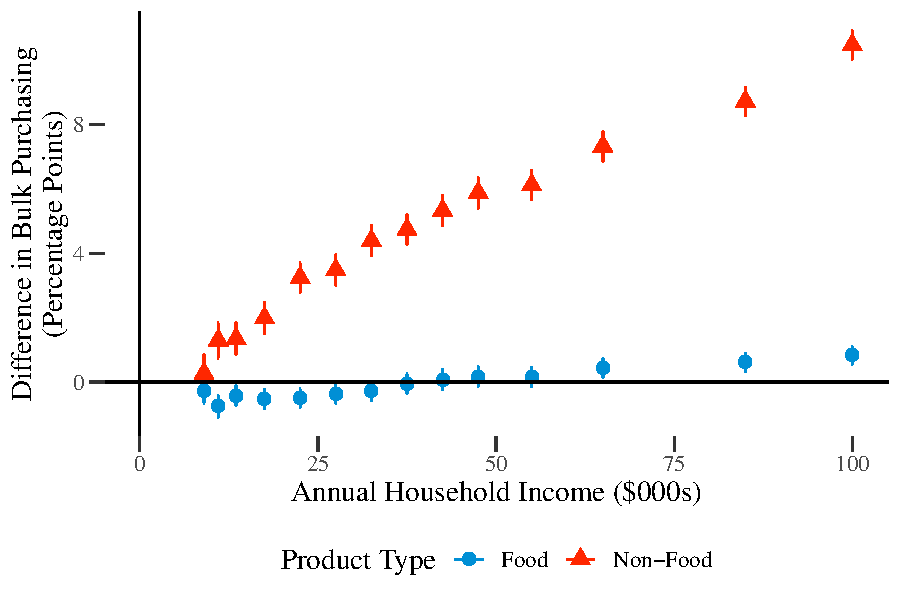
\includegraphics[width = 5in, height = 3in]{../5_figures/savingsBehavior.pdf}
\begin{figurenotes}
Figure plots the income bin coefficients from Equation (\ref{eq:discountingBehavior}), which regresses the share of annual purchases that were bulk packages on household characteristics as well as market and year fixed effects. Nielsen projection weights are used to ensure national representativeness. Households making \$5--\$8k are the reference group. Coefficient values are reported in Appendix Tables \ref{tab:discountingBehaviorFood} and \ref{tab:discountingBehaviorNonFood}. 95\% confidence intervals are shown.
\end{figurenotes}
\begin{figurenotes}[Source]
Nielsen Consumer Panel (2004--2017)
\end{figurenotes}
\label{fig:savingsBehavior}
\end{figure}

The 10 percentage point gap is quite large. For the average household making between \$5,000--\$8,000, 39.6\% of their non-food grocery spending is on bulk packages. Hence, households making over \$100,000 are 26\% more likely to buy in bulk relative to the lowest-income group.

These patterns are consistent with high-income households buying in bulk, obtaining low unit prices, and consuming out of storage. Given the existence of quantity discounts, larger packages generally correspond to lower unit prices. The fact that low-income households are less likely to buy these storable items in bulk suggests that some obstacles may prevent them from buying and storing large packages.\footnote{This relationship persists across most categories. Appendix \ref{appendix:bulkGapCategories} shows the same pattern for a few popular categories and Figure \ref{fig:discountingBehaviorChannelNonFood} illustrates the difference for all non-food categories.}

Because the bulk buying gap is largest for non-food products, the rest of this paper focuses on non-food products. These products are ideal for analyzing bulk purchasing because they isolate the key features that make bulk buying and quantity discounts attractive for households. Primarily, households can store items for future consumption. Additionally, these products generally do not have substitutes and they cannot be produced at home (e.g., toilet paper, diapers). My findings carry over to food products, but one must be careful to account for perishability, which counteracts product storability. Additionally, many food products have close substitutes (e.g., soda, juice, water) and home production (e.g., cooking meals) can substitute for many products \citep{aguiar2005, aguiar2007aer}.

\subsection{Savings from Bulk Buying}
%  This uses the tpLowestPrice.R script
%  This uses the otherModsLowestPrice.R script
%  This uses the bulkDiscountSavingsEstimated.R script

In this subsection, I calculate the savings that low-income households could achieve from buying in bulk like high-income households. For each product category, I compute the average difference in package sizes purchased by estimating the following regression:
\begin{equation}
\label{eq:discountingBehavior2}
\ln({AvgSize})_{imt} = \alpha + \sum_q \beta^q Income_{imt} + \gamma X_{imt} + \lambda_m + \lambda_t + \epsilon_{imt},
\end{equation}
where $AvgSize_{imt}$ is the quantity-weighted average package size purchased by household $i$ in market $m$ in year $t$, where a market is a DMA.\footnote{Average package size is weighted by quantity to account for the fact that an unweighted average would favor small packages.} $Income_{imt}$ is an indicator for a household's income quartile. $X$ controls for household characteristics. Market and year fixed effects are included through $\lambda_m$ and $\lambda_t$.

In this regression, $\beta^q$ gives the average log-difference between the package size purchased by a household in income quartile $q$ and the lowest-income quartile (households making less than \$25,000).\footnote{I use quartiles to reduce the number of income bins from 15 to 4, but results hold at more granular levels. Disaggregated results are available upon request.} To compute savings, I multiply this average difference in package size purchased by the category-specific quantity discount estimated in Section \ref{prevalence}. For example, high-income households buy 30\% larger packages of toilet paper which has a quantity discount of 0.216. Therefore, low-income households could save $0.3 \times 0.216 = 0.0648$ or 6.5\% from buying big packages like high-income households do. Aggregating across all categories where high-income households buy larger packages gives an estimated savings of 5\%, or \$215, per year.\footnote{This averages only across categories where high-income households buy larger packages. There are some categories, such as septic tank cleaners, in which high-income households buy in smaller packages. Imposing that low-income households buy the same average size across \textit{all} categories reduces projected savings to 2.3\%.}\footnote{The first-best calculations of savings would identify the product with the lowest unit price given a household's brand and store choice and compute savings based on that product. This estimate will likely be substantially higher than what I computed, so I view the estimated 5\% savings as a conservative estimate of potential savings. See Appendix \ref{excessSpending} for calculations of savings on popular product categories.}

Saving 5\% on these common household purchases is substantial for low-income households. For the bottom quintile of the income distribution, these items account for 30\% of their discretionary spending compared to 19\% for the top quintile of the distribution.\footnote{Discretionary spending is defined as total expenditures minus expenditures on shelter, utilities, transportation, healthcare, cash contributions, personal insurance, and pensions. Calculation is based on expenditure data on food at home and housekeeping supplies from Table 1 of the 2017 Consumer Expenditure Survey available at https://www.bls.gov/opub/reports/consumer-expenditures/2017/home.htm} If the 24.4 million households making under \$25,000 were to obtain these savings, that would be an overall savings of \$5.4 billion annually, assuming no supply-side response.\footnote{Household count comes from Table B19001 of the 2017 1-year American Community Survey.} For context, this is equal to 8\% of the \$68 billion federal Supplemental Nutrition Assistance Program budget in 2017 \citep{snap2019}. These potential savings do not require low-income households to buy more over the course of the year because buying in bulk does not necessarily change how much households \textit{consume}. It just changes how much they \textit{buy} at one time.

\section{Factors Affecting Bulk Buying}
\label{factors}

In this section, I show that \textit{cognitive costs}, \textit{store preferences}, \textit{budget constraints}, and \textit{storage costs} affect the bulk buying decision. To do this, I use plausibly exogenous variation and natural experiments to estimate the causal impact of unit pricing regulation and warehouse club entry on bulk purchasing. Since the biggest differences in bulk buying are for non-food grocery items, all analysis is restricted to non-food products.

\subsection{Cognitive Costs}
\label{salience}

Cognitive costs are the first possible contributor to the bulk buying decision. Consumers may not be aware of the quantity discount (or how valuable it is) because they do not compute unit prices when making purchases. To test this hypothesis, I utilize a novel hand-collected dataset of state-level unit-price regulations requiring retailers to display per-unit prices. Displaying per-unit prices reduces cognitive costs and households can more easily compare products and pick the one with the best value.

Unit price labeling dates back to the late 1960s and early 1970s. During this period, a large consumer protection movement pushed for unit prices to be posted so consumers could compare different brands and sizes of products \citep{miyazaki2000}. As a result, some states passed laws requiring retailers to display unit prices. These laws varied widely with some giving retailers discretion over how to display unit prices and other states specifying formatting requirements, such as minimum font sizes and background colors to aid readability and clarity \citep{rose2000}.

Using annual regulatory updates published by the National Institute of Standards and Technology (NIST), I compile state-level regulations on unit pricing \citep{nist130}. For states with regulations, I cross-check NIST's designation with state regulatory codes and consult with state officials to ensure accuracy. Figure \ref{fig:unitPriceLaws} shows that, as of 2017, 16 states have regulations on the display of unit prices and 34 have no regulations.\footnote{Summary statistics of these groups are reported in Appendix Table \ref{tab:summaryStatsUnitLaws}.}

\begin{figure}[!htb]
\centering
\caption{Unit Price Regulations by State (2017)}
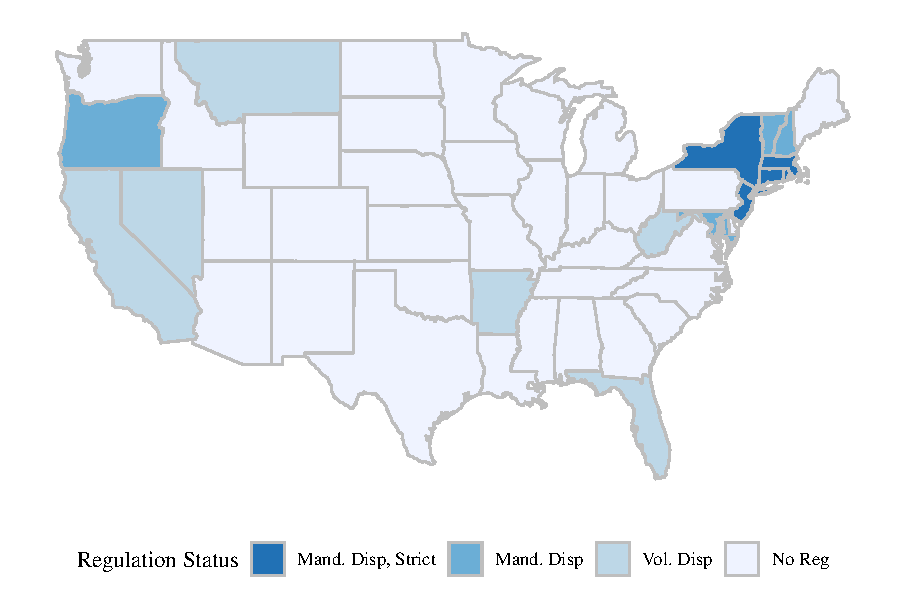
\includegraphics[width = 5in, height = 3in]{../5_figures/unitPriceLaws.pdf}
\begin{figurenotes}
Figure plots whether or not a state has regulations in place governing the display of unit prices as of August 1, 2017. ``No Reg'' denotes that no regulations are in effect. ``Vol. Disp'' denotes states where regulations apply if retailers choose to display unit prices. ``Mand. Disp'' denotes states where all retailers must display unit prices. ``Mand. Disp, Strict'' denotes states where strict display formatting requirements are in effect.
\end{figurenotes}
\begin{figurenotes}[Source]
NIST Handbook 130
\end{figurenotes}
\label{fig:unitPriceLaws}
\end{figure}

If these regulations affect household decisions, then bulk buying should differ between states with and without these regulations. I first document how aggregate patterns in bulk buying differ between states with different regulations and then I will provide causal evidence for the impact of these regulations. I estimate the following regression:
\begin{equation}
\label{eq:unitPrice}
BulkShare_{it} = \alpha + \beta_1 Reg_{it} + \gamma X_{it} + \lambda_t + \epsilon_{it},
\end{equation}

where $BulkShare_{it}$ is the annual share of expenditures that were bulk purchases for household $i$ in year $t$. $Reg_{it}$ is an indicator for whether or not unit-price regulations are in effect. $X_{it}$ controls for household characteristics. I control for year fixed effects through $\lambda_t$. Standard errors are clustered by state because these regulations are at the state level.

Since 2004, no state has modified its regulations on unit prices, so the coefficient on unit pricing regulation is identified from cross-sectional variation between states that have regulations and those that do not.\footnote{Because there is no time variation in regulations, I cannot include state fixed effects in the estimation.}\footnote{In 2013, the District of Columbia passed a law requiring retailers to display unit prices, but no households in my sample live in DC.} Columns (1) and (2) of Table \ref{tab:unitPriceLaw} reveal that bulk purchasing is 3.6 percentage points higher in states with unit price regulations compared to states without unit price regulation, even after controlling for household characteristics and year fixed effects.


% Table created by stargazer v.5.2.2 by Marek Hlavac, Harvard University. E-mail: hlavac at fas.harvard.edu
% Date and time: Wed, Mar 18, 2020 - 11:28:26 AM
\begin{table}[!htbp] \centering 
  \caption{} 
  \label{} 
\begin{tabular}{@{\extracolsep{5pt}}lcccc} 
\\[-1.8ex]\hline 
\hline \\[-1.8ex] 
\\[-1.8ex] & (1) & (2) & (3) & (4)\\ 
\hline \\[-1.8ex] 
 Regulation & 0.035$^{**}$ & 0.036$^{**}$ &  &  \\ 
  & (0.017) & (0.016) &  &  \\ 
  Vol. Disp &  &  & 0.050$^{*}$ & 0.011 \\ 
  &  &  & (0.027) & (0.010) \\ 
  Mand. Disp &  &  & 0.038$^{***}$ & 0.038$^{***}$ \\ 
  &  &  & (0.009) & (0.009) \\ 
  Mand. Disp, Strict &  &  & 0.028$^{***}$ & 0.028$^{***}$ \\ 
  &  &  & (0.006) & (0.006) \\ 
 \hline \\[-1.8ex] 
Avg Bulk & 0.5 & 0.5 & 0.5 & 0.49 \\ 
Demographics & N & Y & Y & Y \\ 
Omit California & N & N & N & Y \\ 
Observations & 732,512 & 732,512 & 732,512 & 668,791 \\ 
Adjusted R$^{2}$ & 0.006 & 0.057 & 0.045 & 0.037 \\ 
\hline 
\hline \\[-1.8ex] 
\textit{Note:}  & \multicolumn{4}{l}{$^{*}$p$<$0.1; $^{**}$p$<$0.05; $^{***}$p$<$0.01} \\ 
\end{tabular} 
\end{table} 


I then analyze these unit pricing regulations at a higher level of detail. State regulations vary across two dimensions: Posting and Formatting. Table \ref{tab:unitPriceLawTable} shows the breakdown of states along these dimensions. First, states can opt to have unit price posting be voluntary (seven states) or mandatory (nine states). Second, states can specify how unit prices are formatted when they are displayed.\footnote{All states with these regulations standardize how unit prices are to be calculated, which is what makes the voluntary states different from states without regulations.} Formatting regulations specify features including minimum font sizes, background colors, and label positioning. With the exception of California, only states that mandate unit price posting have formatting requirements. Excluding California, regulations are naturally ordered: no regulation, voluntary posting, mandatory posting (no formatting requirements), and mandatory posting (with formatting requirements).

\begin{table}[!htbp] \centering
\caption{Unit Price Regulations by State}
\label{tab:unitPriceLawTable}
\begin{tabularx}{\textwidth}{l|XX|XX|}

    \multicolumn{1}{l}{}  & \multicolumn{2}{c}{No Formatting Rules} & \multicolumn{2}{c}{Strict Formatting Rules} \\
    \cline{2-5}
  Voluntary & Arkansas & Montana & California & \\
  Posting   & Florida   & Nevada &            & \\
            & Hawai'i & West Virginia &       & \\
               \cline{2-5}
 Mandatory & Maryland & Vermont & Connecticut & New York \\
 Posting    & \multicolumn{2}{l|}{New Hampshire}    & Massachusetts & Rhode Island \\
            & Oregon        &   & New Jersey    &       \\
                            \cline{2-5}
\end{tabularx}
\begin{tablenotes}
Table reports whether unit price posting is mandatory or voluntary for retailers and whether or not there are strict formatting requirements on how unit prices should be displayed (minimum font size, color, etc.).
\end{tablenotes}
\end{table}


Columns (3) and (4) continue the earlier analysis, but leverage the stringency of the regulations. Column (3) shows that mandatory posting is associated with significantly higher bulk buying, but states with voluntary requirements may have higher rates of bulk buying. However, as Table \ref{tab:unitPriceLawTable} shows, California is an outlier in this regulatory environment because is the only state with the unique combination of voluntary posting and strict formatting requirements. Because of this, I exclude California and re-estimate the regression. Column (4) reveals that California is the primary driver of this effect and states with voluntary posting do not have significantly higher bulk purchasing. On the other hand, mandatory unit price posting is associated with a 2.8--3.8 percentage point increase in bulk buying. The point estimates for bulk buying in states with strict formatting requirements are lower than those in states without formatting requirements, but these estimates are not significantly different from each other. This pattern supports the intuition that standardized unit price presentation reduces cognitive costs, increases the salience of unit prices, and facilitates comparisons for consumers.

This estimation provides strong evidence of a relationship between unit pricing regulations and bulk purchasing. However, there is a risk of selection bias since these regulations were primarily adopted in the Northeast and West Coast regions of the United States. To provide causal evidence, I examine about 13,000 households that move once during their tenure in the data. About 11\% of these households move between regulatory regimes while the remainder are either local moves or moves that maintain their current regulatory regime. To estimate the effect of unit-price regulations on these movers, I use a differences-in-differences specification:
\begin{equation}
\label{eq:unitPriceMove}
BulkShare_{it} = \alpha + \beta_1 Reg_{it} + \gamma X_{it} + \lambda_i + \lambda_t + \epsilon_{it},
\end{equation}
where the variables are the same as in Equation (\ref{eq:unitPrice}), but I control for household fixed effects and standard errors are clustered at the household level.\footnote{Clustering at the state level does not affect the estimates.} With this specification, $\beta_1$ is identified by changes in bulk purchases for households that move from a state with unit-price regulations to a state without unit-price regulations (or vice versa).\footnote{Projection weights are not used because the weights are not designed for this subsample of movers.} Since the ``direction'' of a household's move may matter (i.e., whether they start in a state without regulations and move to a state with regulations or vice versa), in subsequent specifications, I will account for the direction of the move.\footnote{Appendix Table \ref{tab:summaryStatsUnitLawsMovers} reports summary statistics for various groups of movers. Groups are relatively similar, but movers are slightly richer, older, more educated, and have fewer children.}

This specification relies on the assumption that households would have continued buying in bulk like other households that moved, but did not change their regulatory regime. To provide evidence supporting this ``common trends'' assumption, I plot an event study by estimating a modified version of Equation (\ref{eq:unitPriceMove}):
\begin{equation}
\label{eq:unitPriceEventStudy}
BulkShare_{it} = \alpha + \sum_{\tau \neq -1} \beta_1^\tau Yr_{it} + \gamma X_{it} + \lambda_i + \lambda_t + \epsilon_{it},
\end{equation}
where $Yr$ is a dummy for each year before or after a household moves to a state with a different unit pricing regime. The reference group is $t = -1$ so all effects are relative to the year before the household moves. Figure \ref{fig:unitPriceEventStudy} plots the annual coefficients. Figure \ref{fig:unitPriceEventStudy} shows that there are no significant pre-trends. Furthermore, households decrease their bulk buying when they move from a state with unit-price regulations to a state without unit-price regulations. On the other hand, households that move from states without unit-price regulations to states with unit pricing regulations do not significantly change their bulk buying.

\begin{figure}[!htb]
\centering
\caption{Event Study of Movers and Unit Price Regulations}
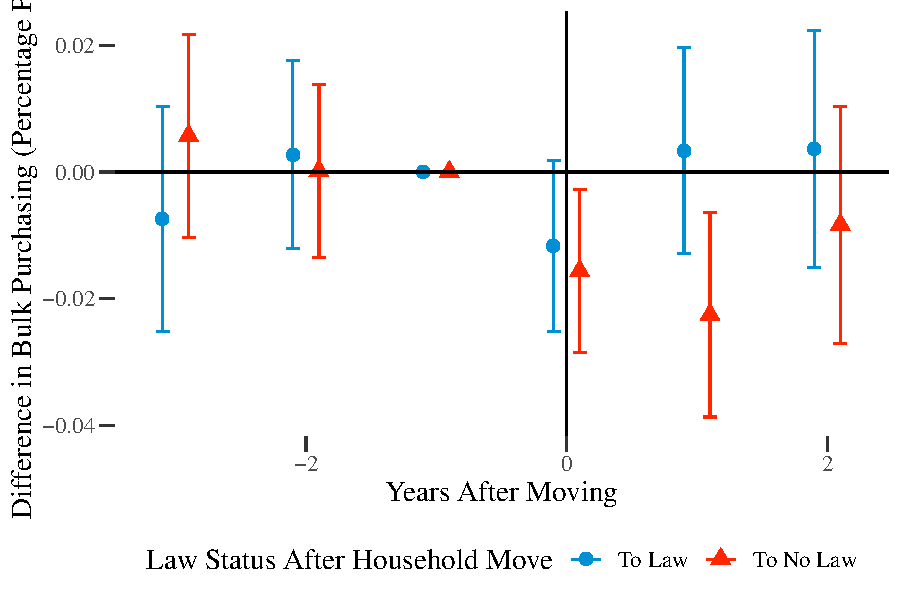
\includegraphics[width = 5in, height = 3in]{../5_figures/unitPriceEventStudyColor.pdf}
\begin{figurenotes}
Figure plots the $\beta_1^t$ coefficients and 95\% confidence intervals from Equation (\ref{eq:unitPriceEventStudy}), which regresses household bulk purchasing on dummies for years before and after a household moves to a state with a different unit pricing regime than the state it moves from. The regression controls for household characteristics as well as household and year fixed effects. Standard errors are clustered at the household level. ``To'' reports estimates for households that move from a state without unit price regulations to a state with unit price regulations. ``Away'' reports estimates for households that move from a state with unit price regulations to a state without regulations.
\end{figurenotes}
\begin{figurenotes}[Source]
Nielsen Consumer Panel (2004--2017)
\end{figurenotes}
\label{fig:unitPriceEventStudy}
\end{figure}

Table \ref{tab:unitPriceLawMovers} reports the results of estimating Equation (\ref{eq:unitPriceMove}). Columns (1) and (2) show that a household's bulk buying is about one percentage point higher when they are in a state with unit price regulations, but this effect is only marginally significant. This specification implicitly assumes that the effect of moving to a state with unit price regulations will be the same as moving to a state without regulations (i.e., the effect is symmetric). Column (3) treats the different directions of moving differently and shows that moving to a state without unit price regulations significantly decreases bulk buying by 1.4 percentage points while moving to a state with regulations does not significantly change bulk buying.

\begin{table}[!htbp] \centering
  \caption{Event Study of Movers to Different State Regulatory Regimes}
  \label{tab:unitPriceLawMovers}
\begin{tabular}{@{\extracolsep{5pt}}lcccc}
\\[-1.8ex]\hline
\hline \\[-1.8ex]
 & \multicolumn{2}{c}{All Households} & No Law To Law & Law To No Law \\
\\[-1.8ex] & (1) & (2) & (3) & (4)\\
\hline \\[-1.8ex]
 Regulation & 0.011$^{***}$ & 0.013$^{***}$ & 0.004 & 0.022$^{***}$ \\
  & (0.004) & (0.004) & (0.006) & (0.006) \\
 \hline \\[-1.8ex]
Household FE & Y & Y & Y & Y \\
Year FE & Y & Y & Y & Y \\
Demographics & N & Y & Y & Y \\
Observations & 731,762 & 731,762 & 723,926 & 723,394 \\
Adjusted R$^{2}$ & 0.658 & 0.659 & 0.659 & 0.659 \\
\hline
\hline \\[-1.8ex]
\textit{Note:}  & \multicolumn{4}{l}{$^{*}$p$<$0.1; $^{**}$p$<$0.05; $^{***}$p$<$0.01} \\
\end{tabular}
\caption*{Notes: Using 2004--2017 Nielsen Consumer Panel data and state-level regulations, this table shows estimates of Equation \ref{eq:unitPriceMove} which regresses household bulk buying on unit price regulation after controlling for household fixed effects. "Regulation" denotes the estimated effect of moving from a state without regulation to a state with regulation. Columns (3) and (4) only include one set of movers in each specification with the remaining households that do not move. Column (3) excludes households that move to states without unit price regulations to restrict identification of the regulatory effect to households moving to states with regulations. Column (4) excludes households that move to states with unit price regulations to restrict identification of the regulatory effect to households moving to states without regulations. Standard errors are clustered at the household level.}
\end{table}


The asymmetric effect of unit pricing indicates the importance of both cognitive costs and consumer education. For households that move to states without regulation, the negative coefficient suggests that cognitive costs are discouraging households from buying in bulk. For households that move to states with regulation, they may not know how to best use the information provided and therefore consumer education may help them recognize the value of quantity discounts and buy in bulk more.

Unit pricing regulations are relatively simple to implement for both policymakers and retailers. Retailers will bear some initial setup costs of redesigning their price labels, but ongoing costs will likely be similar to current menu costs that firms bear.\footnote{In 1975, the Government Accountability Office (then the General Accounting Office) estimated that implementation and maintenance would cost about 0.1\% of sales \citep{gao1975}. This was estimated before the adoption of bar codes and other efficiency-improving practices of the retail sector. Implementing unit pricing now is likely to cost substantially less than those early estimates.} Adopting unit pricing policies (like those recommended by the National Conference on Weights and Measures) would encourage bulk buying while imposing few costs. These findings support the broader assertion that increasing price transparency allows households to choose products that deliver more value.

\subsection{Store Preferences}
The second potential contributor to the bulk buying gap is \textit{store preferences}; low-income households may not live in areas where bulk sizes are available or may not shop at stores that offer bulk sizes. In this subsection, I provide evidence that the bulk buying gap persists within neighborhoods and within store types. Then, I show that warehouse club entry increases bulk buying by 4.0--7.3\%, but these increases hold only for middle- and high-income households.

\subsubsection{Inequality Within Markets and Retail Chains}
%  This uses the discountingBehaviorFE.R script

If supply factors are the primary driver of the bulk buying gap, then the gap should disappear when comparing households in the same neighborhood since they have the same set of stores to choose from. I show that the bulk buying gap still persists within zip codes. This remaining gap corresponds to the amount that \textit{cannot} be explained by differences in access, at least as approximated by geography.

Even within zip codes, there may be other factors affecting where households shop, such as whether or not a household has a vehicle, access to public transit, or a warehouse club membership. To account for possible differences, I examine how much of the bulk buying gap persists within chains. This exercise assumes that within a chain, households have access to the same assortment of goods \citep{dellavigna2019}. I also examine the bulk buying gap within store types (i.e., ``channel'') to account for the fact that bulk buying differences may primarily be between channels (discount versus dollar) instead of between retailers within a channel (Walmart versus Target).\footnote{Retailer names are only for expository purposes. Retailer identities are anonymized in the Nielsen data.}

I estimate within-zip and within-chain bulk buying gaps using a modified form of Equation \ref{eq:discountingBehavior}:
\begin{equation}
\label{eq:discountingBehaviorFE}
BulkShare_{imt} = \alpha + \sum_q \beta^q Income_{imt} + \gamma X_{imt} + \lambda_{mt} + \epsilon_{imt},
\end{equation}
where $Income_{imt}$ is an indicator for the income bin of household $i$ in market $m$ in year $t$. $X_{imt}$ consists of household characteristics. For the analysis of bulk buying within zip code, $BulkShare_{imt}$ is the share of bulk purchases made by household $i$ in zip code $m$ in year $t$ and $\lambda_{mt}$ is a zip-year fixed effect. For the analysis of bulk buying within retail chains, $BulkShare_{imt}$ is the share of bulk purchases made by household $i$ in retail chain $m$ in year $t$ and $\lambda_{mt}$ is a retail chain-year fixed effect and/or a channel-year fixed effect.

Figure \ref{fig:discountingBehaviorFE} plots the income coefficients with and without fixed effects for each regression. Adding zip-year fixed effects reduces the gap between the highest and lowest income groups by 9\% (from 10.5 percentage points to 9.6 percentage points). Results are virtually unchanged if I use county-year fixed effects instead of zip-year fixed effects. Using channel-year fixed effects reduces the bulk buying gap by a more substantial 66\% (from 7.4 percentage points to 2.5 percentage points). Adding retail chain-year fixed effects on top of channel-year fixed effects does not significantly affect the bulk buying gap. This implies that a large share of the bulk buying gap is related to the \textit{types} of stores households shop at, but not the specific chain they choose within a particular store type.

\begin{figure}[!htb]
\centering
\caption{Bulk Buying Within Zip Codes or Stores}
 \begin{subfigure}{0.5\textwidth}
 \centering
 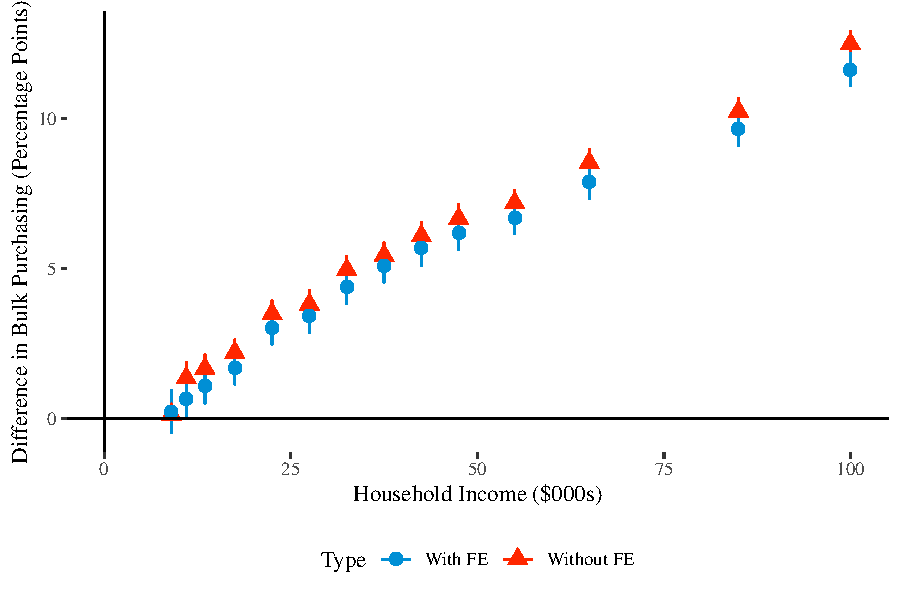
\includegraphics[width = 0.9\linewidth]{../5_figures/discountingBehaviorFEZIPColor.pdf}
 \caption{Zip-Year Fixed Effects}
 \end{subfigure}%
 \begin{subfigure}{0.5\textwidth}
 \centering
 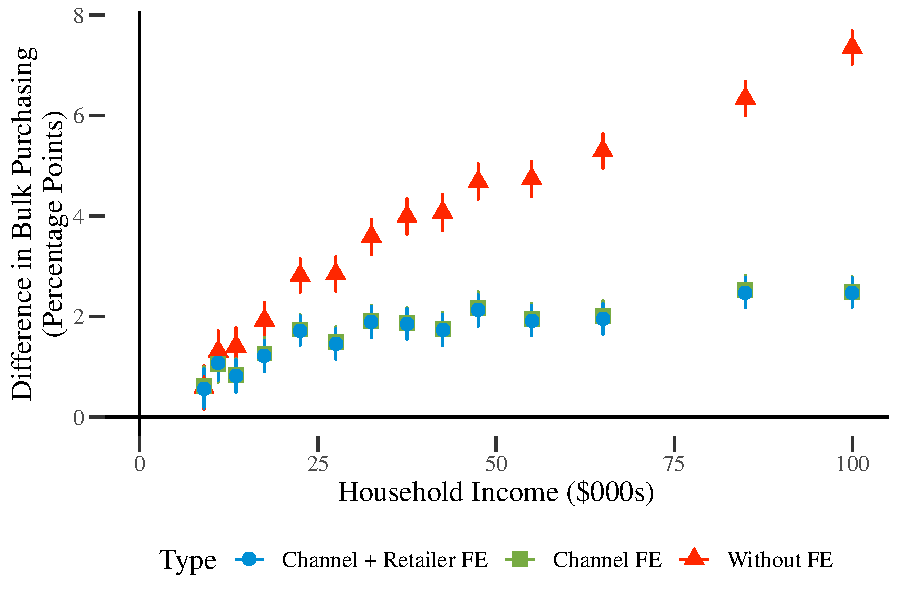
\includegraphics[width = 0.9\linewidth]{../5_figures/discountingBehaviorFEColor.pdf}
 \caption{Retailer/Channel-Year Fixed Effects}
 \end{subfigure}
 \begin{figurenotes}
Figure plots the income bin coefficients from Equation (\ref{eq:discountingBehaviorFE}), which regresses the share of annual purchases that were bulk packages on household characteristics as well as either zip code-year, retailer-year, or channel-year fixed effects (a ``channel'' is a type of store). Nielsen projection weights are used to ensure national representativeness. Households making \$5--\$8k are the reference group. Coefficient values are reported in Table \ref{tab:discountingBehaviorFEAll}.
\end{figurenotes}
\begin{figurenotes}[Source]
Nielsen Consumer Panel (2004--2017)
\end{figurenotes}
\label{fig:discountingBehaviorFE}
\end{figure}

Overall, within zip codes, the bulk buying gap between high- and low-income households persists. However, within store type (or retail chain), the bulk buying gap is substantially reduced. Two important conclusions can be drawn from these patterns. First, in an accounting sense, the type of store a household shops at accounts for two-thirds of the bulk buying gap. This is likely an overestimate of the contribution of store preferences because those preferences may be driven by more fundamental factors (e.g., high storage costs or budget constraints could prevent households from shopping at warehouse clubs, as opposed to households having a low preference for warehouse clubs). Second, the bulk buying gap \textit{still persists} within channels and retail chains. These patterns suggest that where a household shops and what they choose within a store are much more important than where a household is located. The next section explores how store preferences are related to income and how warehouse clubs affect bulk buying.

\subsubsection{Store Preferences by Income}
\label{sec:storePrefs}
%  This uses the expendituresByChannel.R script

The previous section shows that while the bulk buying gap persists within zip codes, it is narrower within store types and retail chains. In this section, I show that the biggest shopping differences between income groups are related to warehouse clubs. I then estimate the effect of warehouse club entry on bulk buying.

To demonstrate differences in store preference by household income, I examine the relationship between where households shop and their income using the following regression:
\begin{equation}
\label{eq:storePreference}
ChannelShare_{imt} = \alpha + \sum_q \beta^q Income_{imt} + \gamma X_{imt} + \lambda_{m} + \lambda_t + \epsilon_{imt},
\end{equation}
where $ChannelShare_{imt}$ is the share of annual spending that household $i$ in market $m$ in year $t$ made in a particular channel (grocery store, discount store, dollar store, drug store, or warehouse club). $Income_{imt}$ is an indicator for a household's income bin. $X_{imt}$ captures other household characteristics. Finally, market and year fixed effects capture differences in spending shares across markets and over time.

\begin{figure}[!htb]
\centering
\caption{Annual Spending Shares By Store Type, Relative to Low-Income Households}
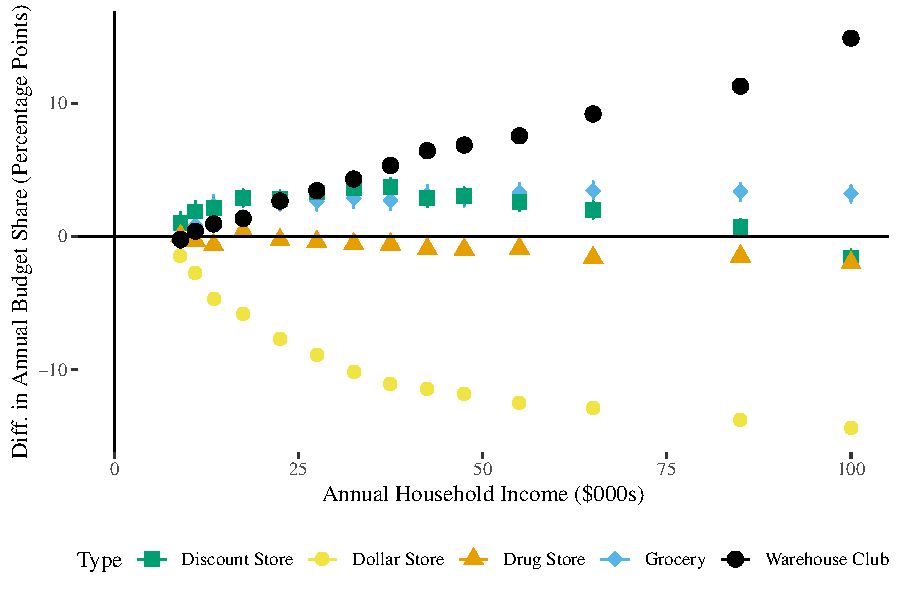
\includegraphics[width = 5in, height = 3in]{../5_figures/expendituresByChannelColor.pdf}
\begin{figurenotes}
Figure plots the income bin coefficients from Equation (\ref{eq:storePreference}), which regresses the share of annual purchases at each store type on household characteristics as well as year and market fixed effects. Nielsen projection weights are used to ensure national representativeness. Households making \$5--8k are the reference group.
\end{figurenotes}
\begin{figurenotes}[Source]
Nielsen Consumer Panel (2004--2017)
\end{figurenotes}
\label{fig:expendituresByChannel}
\end{figure}

Figure \ref{fig:expendituresByChannel} reveals that while there are small differences in the share of annual expenditures at grocery, drug, and discount stores, there are dramatic differences in whether households shop at warehouse clubs or dollar stores: households making over \$100,000 spend about 13 percentage points more of their non-food expenditures at warehouse clubs than households making under \$25,000.

Because the biggest differences are in warehouse clubs and these stores almost solely stock bulk sizes, I focus on how warehouse clubs affect bulk buying. The following analysis of warehouse clubs uses data on over 1,400 warehouse club locations between 2004--2015.\footnote{Data provided by the authors of \citet{coibion2017} and covers BJ's, Costco, and Sam's Club.} The first possibility is that high-income households shop at warehouse clubs because they are closer. Table \ref{tab:costcoDist} shows that low-income households are about 15 miles away from the nearest warehouse club compared to only 8 miles away for high-income households.

\begin{table}[!htbp] \centering
\caption{Average Distance to Warehouse Club by Income (Miles)}
\label{tab:costcoDist}
\begin{tabular}{@{\extracolsep{4pt}}lcccc}
\hline
Household Income  & Mean  & SD    & 25th Pctile  & 75th Pctile    \\
\hline
$<$25k            & 14.79 & 18.98 & 3.26 & 20.53    \\
25-50k            & 12.79 & 17.51 & 3.03 & 15.94  \\
50-100k           & 10.61 & 15.16 & 2.85 & 12.01  \\
$>$100k             & 7.92  & 12.08 & 2.51 & 8.45   \\
\hline
\hline
\end{tabular}
\begin{tablenotes}
Table reports the distance between zip code centroids of warehouse locations and household locations. Nielsen projection weights are used to ensure national representativeness.
\end{tablenotes}
\begin{tablenotes}[Source]
Nielsen Consumer Panel (2004--2015)
\end{tablenotes}
\end{table}


The ideal experiment would randomly assign warehouse clubs to neighborhoods and then their effect on bulk buying could easily be calculated. Even though store locations are not randomly assigned, within a household, it is exceedingly unlikely that a warehouse club opening could be co-incident with a shift in bulk buying, so any observed changes are likely causal. Leveraging the panel structure of the Nielsen Consumer Panel, I estimate how a household's bulk purchasing changes after a warehouse club opens using the following equation:
\begin{equation}
\label{eq:costcoEntry}
BulkShare_{imt} = \alpha + \beta Entry_{imt} + \gamma X_{imt} + \lambda_{im} + \lambda_{t} + \epsilon_{imt},
\end{equation}
where $BulkShare_{imt}$ is the share of bulk purchases made by household $i$ in market $m$ in quarter $t$. $Entry_{imt}$ is an indicator for whether or not a warehouse club entered within 15 miles of household $i$ in quarter $t$.\footnote{In cases where a household is located near multiple warehouse clubs, I use the earliest entry date since the first warehouse club would generate the largest supply shock.}\footnote{According to the 2017 National Household Travel Survey, the average household traveled about seven miles to buy goods, with low-income households traveling about one or two miles less than higher-income households \citep{nhts2017}. Allowing for the possibility that households might travel farther to shop at a warehouse club, I use a cutoff of 15 miles. Appendix Table \ref{tab:appendixCostcoEntryDifferentRadii} shows that this pattern is robust to other cutoffs.} I include a household-market and year-quarter fixed effects $\lambda$ to ensure that $\beta$ is identified by within-household changes in bulk buying before and after a warehouse club opens instead of households that may move to areas closer to warehouse clubs. $X$ controls for possible demographic changes within the household.

This specification relies on the assumption that households would have continued buying in bulk like other households that did not experience a warehouse club entry. To provide evidence supporting this ``common trends'' assumption, I plot an event study by estimating a modified version of Equation \ref{eq:costcoEntry}, but replace the entry indicator with dummies for each quarter pre- and post-entry:
\begin{equation}
\label{eq:costcoEventStudy}
BulkShare_{imt} = \alpha + \sum_q \beta^q Qtr_{imt} + \gamma X_{imt} + \lambda_{im} + \lambda_t + \epsilon_{imt},
\end{equation}
where $Qtr_{imt}$ is a dummy for each quarter prior to entry and after entry, with the quarter immediately before entry ($q = -1$) as the reference group. Figure \ref{fig:eventStudyIncome} plots the quarterly coefficients and shows that for most income groups there are no significant pre-trends. For households in the lowest income quartile, there is some evidence that those that experienced a warehouse club entry buy in bulk more often than other low-income households that do not experience an entry. After a warehouse club enters, there are significant increases in bulk buying for middle- and high-income households and these effects are persistent up to eight quarters after a warehouse club has opened.

\begin{figure}[!htb]
\centering
\caption{Event Study of Warehouse Club Entry}
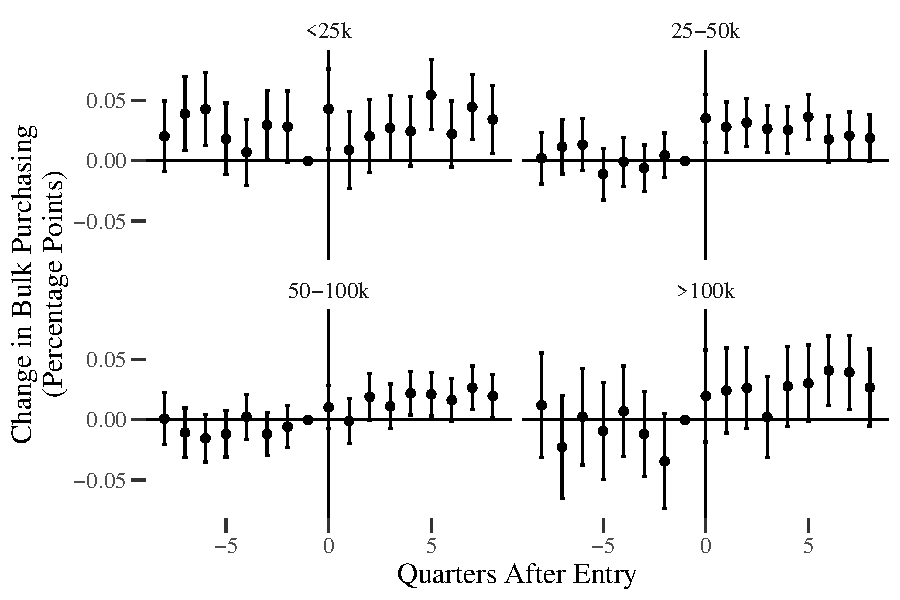
\includegraphics[width = 4.9in, height = 3in]{../5_figures/eventStudyIncome15Mi.pdf}
\begin{figurenotes}
Figure plots the quarterly coefficients from Equation (\ref{eq:costcoEventStudy})---the effects of warehouse club entry on bulk purchasing of households before and after warehouse club entry---using 2004--2015 household-by-quarter Nielsen Consumer Panel data. The regression controls for household characteristics as well as household-zip code fixed effects. All coefficients are relative to bulk purchasing in the quarter before entry ($q = -1$). Error bars denote 95\% confidence intervals.
\end{figurenotes}
\label{fig:eventStudyIncome}
\end{figure}

Table \ref{tab:costcoEntryDD} shows the regression results. Overall, households that experienced a warehouse club entry increased their bulk purchasing by two percentage points. However, when I interact household income with warehouse club entry, the increase in bulk buying is due to changes for households making over \$25,000 and is increasing in income, with households making over \$100,000 increasing their bulk buying by 3.5 percentage points. Households in the lowest quartile do not have any significant change in their bulk buying. One likely reason that low-income households do not change their bulk buying is that even after a warehouse club enters, households do not purchase a membership (fees range from \$45--\$120 depending on the chain and membership level). Other possible reasons are that low-income households do not have access to transportation that can carry items home, do not have the space to store the items, or even if they had a membership, they still would not purchase extremely large sizes available at warehouse clubs due to budget constraints.\footnote{As an example, Philadelphia provides public transit access to a warehouse club. However, carrying club-sized items on a bus is infeasible for more than two or three items. A personal vehicle would be necessary.}

\begin{table}[!htbp] \centering
  \caption{Effect of Warehouse Club Entry on Bulk Buying}
  \label{tab:costcoEntryDD}
\begin{tabular}{@{\extracolsep{5pt}}lccc}
\\[-1.8ex]\hline
\hline \\[-1.8ex]
\\[-1.8ex] & (1) & (2) & (3)\\
\hline \\[-1.8ex]
 Post-Entry & 0.017$^{***}$ & 0.017$^{***}$ & $-$0.005 \\
  & (0.004) & (0.004) & (0.007) \\
  Post-Entry : 25-50k &  &  & 0.022$^{***}$ \\
  &  &  & (0.008) \\
  Post-Entry : 50-100k &  &  & 0.028$^{***}$ \\
  &  &  & (0.009) \\
  Post-Entry : >100k &  &  & 0.039$^{***}$ \\
  &  &  & (0.012) \\
 \hline \\[-1.8ex]
Household-ZIP FE's & Y & Y & Y \\
Year-Quarter FE's & Y & Y & Y \\
Demographic Controls & N & Y & Y \\
Observations & 2,520,129 & 2,520,129 & 2,520,129 \\
Adjusted R$^{2}$ & 0.427 & 0.427 & 0.427 \\
\hline
\hline \\[-1.8ex]
\textit{Note:}  & \multicolumn{3}{l}{$^{*}$p$<$0.1; $^{**}$p$<$0.05; $^{***}$p$<$0.01} \\
\end{tabular}
\caption*{Notes: This table uses 2004--2015 Nielsen Consumer Panel data at the household-quarter level. Coefficients are reported for Equation (\ref{eq:costcoEntry}) which regresses households' quarterly bulk purchase shares on an indicator for warehouse club entry, household characteristics as well as household-ZIP code and year-quarter fixed effects are included. Projection weights are not used.}
\end{table}


This analysis estimates the intent to treat effect since not all households shop at the entrant warehouse club after it opens. As a result, this is a conservative lower bound on the actual treatment effect on households that shop at warehouse clubs.\footnote{Even though low-income households do not change their bulk buying, other research suggests that they may be worse off because existing retailers are more likely to increase prices for storable products as a competitive response \citep{bauner2019}.} The effect is quite substantial even given how conservative it is.

To examine whether this change in bulk buying comes from households shopping more at warehouse clubs, I estimate Equation \ref{eq:costcoEntry} on different margins of bulk buying. The increase in bulk buying after warehouse club entry could be coming from three possible margins. First, households could increase their bulk buying at non-warehouse club stores (intensive non-warehouse club margin). Second, households could increase their bulk buying at warehouse club stores (intensive warehouse club margin). Third, households could increase their bulk buying by switching shopping to warehouse club stores (extensive margin). The observations used in estimation are household-quarter bulk shares at warehouse club and non-warehouse club stores.

\begin{table}[!htbp] \centering
  \caption{Effect of Warehouse Club Entry on Bulk Buying Along Different Margins}
  \label{tab:costcoEntryDDMargin}
\begin{tabular}{@{\extracolsep{5pt}}lccc}
\\[-1.8ex]\hline
\hline \\[-1.8ex]
 & Non-Club & Club & Club Intensive \\
\\[-1.8ex] & (1) & (2) & (3)\\
\hline \\[-1.8ex]
 Post-Entry & 0.0001 & 0.075$^{***}$ & $-$0.005 \\
  & (0.004) & (0.007) & (0.004) \\
  Post-Entry : 25-50k & $-$0.003 & 0.018$^{***}$ & $-$0.003 \\
  & (0.004) & (0.006) & (0.004) \\
  Post-Entry : 50-100k & $-$0.001 & 0.009$^{***}$ & 0.0005 \\
  & (0.002) & (0.003) & (0.003) \\
  Post-Entry : $>$100k & $-$0.001 & 0.012$^{***}$ & $-$0.001 \\
  & (0.003) & (0.004) & (0.003) \\
 \hline \\[-1.8ex]
Avg Bulk & 0.4 & 0.27 & 0.97 \\
Household-ZIP FE's & Y & Y & Y \\
Year-Quarter FE's & Y & Y & Y \\
Demographic Controls & Y & Y & Y \\
Observations & 2,401,038 & 2,401,038 & 661,240 \\
Adjusted R$^{2}$ & 0.254 & 0.567 & 0.193 \\
\hline
\hline \\[-1.8ex]
\end{tabular}
\begin{tablenotes}
Table reports coefficient estimates for Equation (\ref{eq:costcoEntry}) which regresses households' quarterly bulk purchase shares on an indicator for warehouse club entry, household characteristics as well as household-zip code and year-quarter fixed effects. Column (1) uses bulk buying shares only at non-warehouse club stores as the dependent variable. Column (2) uses bulk buying shares at warehouse club stores (inclusive of zero spending quarters) as the dependent variable. Column (3) uses bulk buying shares at warehouse club stores (excluding zero spending quarters) as the dependent variable. Projection weights are not used. $^{*}$p$<$0.1; $^{**}$p$<$0.05; $^{***}$p$<$0.01
\end{tablenotes}
\begin{tablenotes}[Source]
Nielsen Consumer Panel (2004--2015)
\end{tablenotes}
\end{table}


Table \ref{tab:costcoEntryDDMargin} shows the regression results. Column (1) is estimated using quarterly bulk buying shares at non-warehouse club stores as the dependent variable. After warehouse club entry, there is no significant change in bulk buying at non-warehouse club stores for any income group. Furthermore, the standard errors are quite small, so if there were changes, they are minimal. Column (2) is estimated using quarterly bulk buying shares at warehouse club stores as the dependent variable, which includes many zeros because there are quarters where households do not shop at warehouse club stores. For households that never shop at warehouse club stores, they have a string of zeroes. After warehouse club entry, quarterly bulk buying at warehouse clubs increases by a statistically significant 7.5 percentage points and is higher for higher income groups. This increase could be generated by households shopping more often at warehouse clubs, and therefore increasing the number of quarters with non-zero bulk spending at warehouse clubs. It could also be generated by households increasing the share of bulk purchases they already make at warehouse clubs. Column (3) focuses on only quarters with positive bulk shares at warehouse clubs and shows that there are no significant changes in bulk buying, conditional on shopping at a warehouse club, after a warehouse club enters. Therefore, the significant increase in Column (2) is generated by households switching to shopping more at warehouse clubs after a warehouse club enters. Overall, warehouse club entry increases bulk buying by encouraging households to make more shopping trips to warehouse clubs.


\subsection{Budget Constraints}
Budget constraints may be another contributing factor to the bulk buying gap. Importantly, the necessary budget constraints must bind over short time periods (e.g., months) because over the course of a year, households spend more than they would have for the same amount of goods if they had taken advantage of bulk discounts. Such short-horizon budget constraints are most binding for the lowest income groups, but are unlikely to bind for middle- and high-income groups.\footnote{Middle- and high-income households may still face monthly budget constraints, but grocery spending is unlikely to be a major factor for all but the lowest-income households.}

To test this explanation, I examine over-the-month changes in liquidity. Low-income households are more likely to have higher liquidity at the start of the month compared to the end of the month \citep{stephens2003, orhun2018}. Consistent with this fact, the spending of low-income households tends to decline over the course of the month while the spending of higher income groups is relatively flat \citep{orhun2018}.

I use within-household variation in the timing of purchases to estimate a
differences-in-differences model. This model tests the coincidence of changes to bulk buying with times of the month when households may be liquidity constrained. This approach is similar to \citet{orhun2018}. I use weekly bulk buying information to estimate the following regression:
\begin{equation}
\label{eq:discountingBehaviorLiquidity}
BulkShare_{iw} = \alpha + \sum_q \sum_{w = 2}^4 \beta_1^{qw} \mathbbm{1}\{week = w\} * Inc_{iw} + \beta_2 Inc_{iw} + \gamma X_{iw} + \lambda_i + \epsilon_{iw},
\end{equation}
where $BulkShare_{iw}$ is the share of bulk purchases made by household $i$ in week $w$. $\mathbbm{1}\{week = w\}$ is an indicator for the second, third, or last week of the month. $Inc_{iw}$ indicates the household's income bin $q$. $X_{iw}$ is the usual set of household characteristics and $\lambda$ is a household fixed effect. The results are reported in Table \ref{tab:discountingBehaviorLiquidity}.

\begin{table}[!htbp] \centering
  \caption{Over-the-Month Changes in Bulk Buying}
  \label{tab:discountingBehaviorLiquidity}
\begin{tabular}{@{\extracolsep{5pt}}lccc}
\\[-1.8ex]\hline
\hline \\[-1.8ex]
\\[-1.8ex] & (1) & (2) & (3)\\
\hline \\[-1.8ex]
 Week 2 & $-$0.002$^{***}$ & $-$0.001 & $-$0.001 \\
  & (0.0004) & (0.001) & (0.001) \\
  Week 3 & $-$0.002$^{***}$ & $-$0.004$^{***}$ & $-$0.004$^{***}$ \\
  & (0.0004) & (0.001) & (0.001) \\
  Week 4 & 0.002$^{***}$ & $-$0.002$^{**}$ & $-$0.002$^{**}$ \\
  & (0.0004) & (0.001) & (0.001) \\
  25-50k &  & 0.003$^{***}$ & 0.002$^{**}$ \\
  &  & (0.001) & (0.001) \\
  Week 2 : 25-50k &  & $-$0.002$^{**}$ & $-$0.002$^{**}$ \\
  &  & (0.001) & (0.001) \\
  Week 3 : 25-50k &  & 0.001 & 0.001 \\
  &  & (0.001) & (0.001) \\
  Week 4 : 25-50k &  & 0.003$^{***}$ & 0.003$^{***}$ \\
  &  & (0.001) & (0.001) \\
  50-100k &  & 0.009$^{***}$ & 0.004$^{***}$ \\
  &  & (0.001) & (0.001) \\
  Week 2 : 50-100k &  & $-$0.001 & $-$0.001 \\
  &  & (0.001) & (0.001) \\
  Week 3 : 50-100k &  & 0.002$^{*}$ & 0.002$^{*}$ \\
  &  & (0.001) & (0.001) \\
  Week 4 : 50-100k &  & 0.005$^{***}$ & 0.005$^{***}$ \\
  &  & (0.001) & (0.001) \\
  >100k &  & 0.025$^{***}$ & 0.012$^{***}$ \\
  &  & (0.001) & (0.001) \\
  Week 2 : >100k &  & 0.001 & 0.001 \\
  &  & (0.001) & (0.001) \\
  Week 3 : >100k &  & 0.006$^{***}$ & 0.006$^{***}$ \\
  &  & (0.001) & (0.001) \\
  Week 4 : >100k &  & 0.007$^{***}$ & 0.007$^{***}$ \\
  &  & (0.001) & (0.001) \\
 \hline \\[-1.8ex]
Mean Bulk & 0.46 & 0.46 & 0.46 \\
Household FE's & Y & Y & Y \\
Demographics & N & N & Y \\
Observations & 2,854,905 & 2,854,905 & 2,854,905 \\
Adjusted R$^{2}$ & 0.402 & 0.402 & 0.404 \\
\hline
\hline \\[-1.8ex]
\textit{Note:}  & \multicolumn{3}{l}{$^{*}$p$<$0.1; $^{**}$p$<$0.05; $^{***}$p$<$0.01} \\
\end{tabular}
\caption*{Notes: Using 2004--2017 Nielsen Consumer Panel data, this table displays the regression coefficients from estimating Equation {eq:discountingBehaviorLiquidity} which regresses a household's weekly share of bulk purchases of non-food products on the week of the month, income, and other household characteristics and includes a households fixed effect.}
\end{table}


Overall, households making less than \$25,000 decrease their bulk buying by a slight 0.2 to 0.4 percentage points during the third and fourth weeks of the month while households making over \$25,000 have no decline (and possibly a slight increase) in their bulk buying during the third and fourth weeks of the month.

This analysis does not rule out the possibility of liquidity constraints contributing to differences in bulk buying, but it does rule out that local changes in liquidity significantly affect bulk buying. Liquidity shocks larger than intra-month paycheck variation may be necessary to increase bulk buying, but more work would be necessary to determine whether that is the case.

\subsection{Storage Costs}
\label{storageCosts}

Storage costs are the fourth contributing factor that I examine. Intuitively, households that buy in bulk need a place to store large packages, which could be in a basement, pantry, or cabinets. Households without available storage space may want to save money through quantity discounts, but choose not to because they have limited storage space.

The ideal experiment would randomly assign households to various home sizes and then observe their bulk purchasing behavior to identify storage costs. However, exogenously changing a household's living situation is infeasible. The next best option is to test some intuitive implications of storage costs. First, while I cannot randomly assign households to different home sizes, there are many households that move while they are in the Nielsen panel. I observe whether households live in single-family homes or apartments, which generates variation in available storage space. According to the American Housing Survey, the median single-family home is about twice as large as the median apartment. Since at least 1999, new single-family homes have had a median size of 2,000--2,400 square feet while the median apartment is only 1,000--1,100 square feet and this holds true within Census regions as well. Therefore, households that move into single-family homes are likely to have more available storage space and this will increase their willingness to buy in bulk.

To test this hypothesis, I estimate how bulk buying changes when households change their housing size, by estimating Equation \ref{eq:storageCosts}:
\begin{equation}
\label{eq:storageCosts}
BulkShare_{it} = \alpha + \beta House_{it} + \gamma X_{it} + \lambda_i + \lambda_t + \epsilon_{it},
\end{equation}
where $House_{it}$ is a dummy for whether a household $i$ lives in a single-family house in year $t$ (apartments are the reference group). $X_{it}$ controls for changes in other household characteristics. Household and year fixed effects, $\lambda$, ensure that $\beta$ is identified off of within-household changes in housing. Standard errors are clustered at the household level. Table \ref{tab:storageCosts} shows that bulk buying is one percentage point higher when households are in single-family homes compared to when they are in apartments.

\begin{table}[!htbp] \centering
  \caption{Relationship Between Bulk Buying and Housing Changes}
  \label{tab:storageCosts}
\begin{tabular}{@{\extracolsep{5pt}}lccc}
\\[-1.8ex]\hline
\hline \\[-1.8ex]
\\[-1.8ex] & (1) & (2) & (3)\\
\hline \\[-1.8ex]
 Single-Family Home & 0.012$^{***}$ & 0.010$^{***}$ & 0.010$^{***}$ \\
  & (0.002) & (0.002) & (0.003) \\
 \hline \\[-1.8ex]
Market FE's & Y & Y & Y \\
Year FE's & Y & Y & Y \\
Demographics & N & Y & Y \\
Future Income & N & N & Y \\
Observations & 731,762 & 731,762 & 566,535 \\
Adjusted R$^{2}$ & 0.687 & 0.687 & 0.690 \\
\hline
\hline \\[-1.8ex]
\textit{Note:}  & \multicolumn{3}{l}{$^{*}$p$<$0.1; $^{**}$p$<$0.05; $^{***}$p$<$0.01} \\
\end{tabular}
\caption*{Notes: Using Nielsen 2004--2017 Consumer Panel data, this table shows the results of estimating Equation \ref{eq:storageCosts}. The dependent variable is the annual share of bulk purchases made by households and the independent variables are housing and other household characteristics. Estimating includes household, market, and year fixed effects. "Future Income" denotes a household's income one year in the future. Standard errors are clustered by household.}
\end{table}


Column (1) shows that bulk buying is 1.2 percentage points higher when a household lives in a single-family home. However, since housing changes can be due to other within-household shifts, such as marriage or having children, column (2) also controls for other within-household demographic changes. The increase in bulk buying is slightly reduced, but there is still an increase when households move into larger spaces. Finally, households may move into larger housing if they expect to earn more and this expectation of future income may also increase their bulk buying. Column (3) also includes a household's one-year-ahead income and there is no change to the bulk buying increase after a household moves into a single-family home. This result is not causal, but it supports the intuition that when households have more storage space, they are more able to buy in bulk.

Another implication of storage costs is that products with a smaller ``footprint'' (physical volume) have lower storage costs. Therefore, if storage costs influence bulk buying, there should be a smaller gap in bulk buying for smaller products (like plastic wrap) relative to large, cumbersome products (like paper towels and toilet paper). To test this implication, I estimate a modified form of Equation \ref{eq:discountingBehavior2} that relates average package sizes with household income:
\begin{equation*}
\ln(AvgSize)_{imt} = \alpha + \sum_q \beta^q Income_{imt} + \gamma X_{imt} + \lambda_m + \lambda_t + \epsilon_{imt},
\end{equation*}
where $AvgSize_{imt}$ is the average package size purchased by household $i$ in market $m$ in year $t$. $Income_{imt}$ consists of dummies for each income quantile $q$. $X_{imt}$ consists of household characteristics. Year and market fixed effects are captured by $\lambda$.

Figure \ref{fig:discountingBehaviorChannelNonFood} plots the income coefficients from the regression for all non-food grocery categories. I have highlighted some popular product categories. The bulk buying gap is largest for the physically biggest products such as paper towels and toilet paper while the gap is smaller for less bulky items such as liquid detergent and diapers. Overall, this pattern supports the hypothesis that storage costs contribute to the bulk buying gap, but the persistence of the gap even for smaller products suggests that other factors are at play.

\begin{figure}[!htb]
\centering
\caption{Bulk Buying Gap For Non-Food Grocery Products}
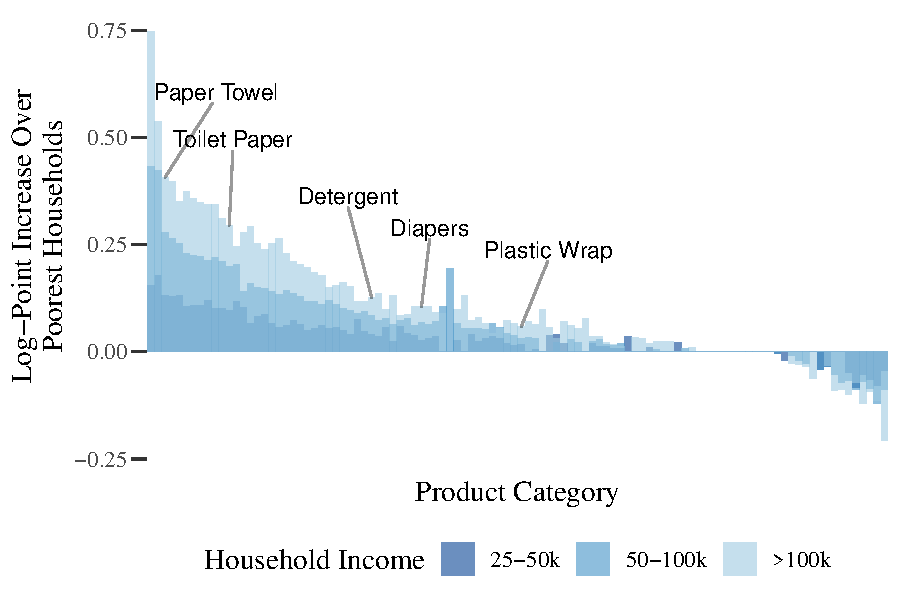
\includegraphics[width = 5in, height = 3in]{../5_figures/discountingBehaviorChannelNonFoodColor.pdf}
\begin{figurenotes}
Figure plots the $\beta$ coefficients from Equation (\ref{eq:discountingBehavior2}), which regresses average package size purchased on household income. The regression controls for household characteristics as well as market and year fixed effects.
\end{figurenotes}
\begin{figurenotes}[Source]
Nielsen Consumer Panel (2004--2017)
\end{figurenotes}
\label{fig:discountingBehaviorChannelNonFood}
\end{figure}

Overall, these results provide evidence that storage costs and bulk buying are related. When households move to larger homes (relative to apartments), they buy more in bulk. Similarly, product categories with larger physical footprints exhibit larger bulk buying gaps relative to product categories with smaller footprints. To more precisely quantify storage costs, I estimate a simple model of the consumer purchase decision.

%   ### Transportation Costs
%   This uses transportationCosts.R script
%   Buying in bulk is difficult if individuals have to carry their purchases home from the store, whether that is walking or using public transport. With this in mind, vehicle access may be an important factor that explains the large differences in bulk buying. In this section, I examine some testable implications of transportation costs. Ideally, I would directly observe and control for vehicle access, but Nielsen does not collect that information.
%
%   The American Community Survey provides tract-level measures of vehicle access. In particular, it asks the primary method of how individuals get to work and answers include car, bus, subway, taxi, walking, bicycle, etc. If respondents answer "car," I assume they have vehicle access.\footnote{This answer does not ensure the respondent owns a car, but it suggests they have a vehicle available for transportation (e.g. carpool).} By this metric, vehicle access is nearly universal. Over 90\% of Nielsen households live in Census tracts with at least 90\% vehicle access. Furthermore, while tract-level vehicle access increases with household income, the differences are insubstantial. The average household making less than \$25,000 lives in a tract with 95\% vehicle access and the average household making over \$100,000 lives in a tract with 96\% vehicle access.
%
%   Another testable implication is that if consumers walk or use public transport to carry purchases home, then those with these limitations will purchase fewer items than those without these limitations. To test this, I tally the number of products purchased on each shopping trip and examine the correlation of items purchased with other household observables. I estimate the following regression:
%
%   \begin{equation}
%   \label{eq:transportationCostsItem}
%   Items_{ismt} = \sum_q \beta^q Income^q_{it} + \gamma X_{it} + \lambda_t + \lambda_m + \epsilon_{ismt},
%   \end{equation}
%
%   where $Items_{ismt}$ is the number of items purchased by household $i$ on shopping trip $s$ in county $m$ in year $t$. $Income^q$ is a dummy for income bin $q$. Other household observables are captured by $X$ (age, household composition, marital status, housing, education, tract-level car access). Year and county fixed effects are captured by $\lambda_t$ and $\lambda_m$.
%
%   Figure \ref{fig:transportationCostsItem} plots the $\beta$ coefficients from Equation \ref{eq:transportationCostsItem}. If transportation costs were the primary factor, we would expect that items purchased would increase until the point where all households have a car and then flatten out beyond that point. The figure illustrates a dramatically different pattern, where the line is flat and then dramatically increases. Households making below \$50,000 purchase roughly the same number of products and then households making above \$50,000 purchase 1 to 3 more items per shopping trip. This pattern is more likely due to store preferences identified in Section \ref{sec:storePrefs} in which higher-income households are more likely to shop at warehouse clubs where they likely purchase more items as well. Lower-income households shop a similar mixes of discount and grocery stores and do not buy substantially different quantities of items.
%
%   \begin{figure}[!htb]
%   \centering
%   \caption{Number of Products Purchased Per Shopping Trip}
%   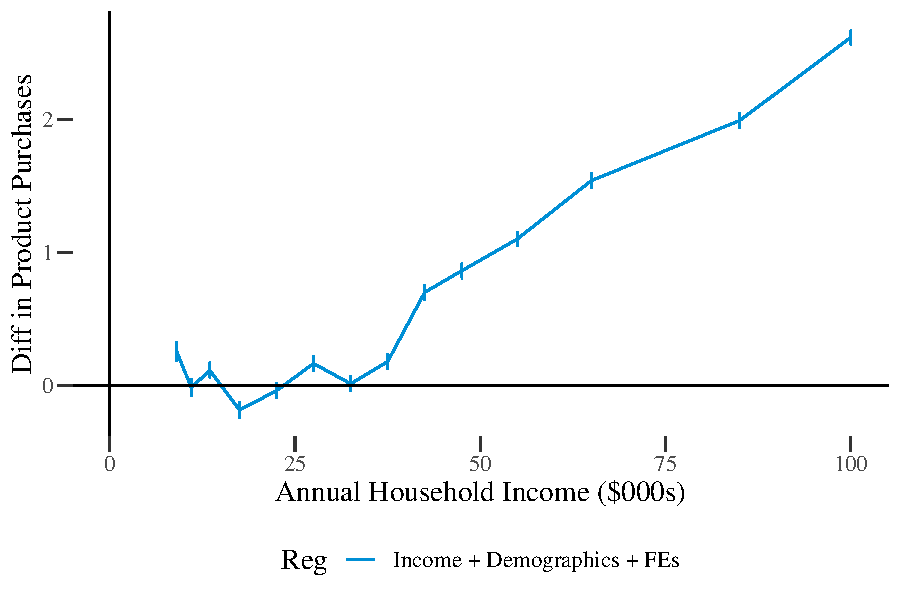
\includegraphics[width = 5in, height = 3in]{../5_figures/transportationCostsItem.pdf}
%   \caption*{Note: Using 2004--2017 Nielsen Consumer Panel data, this figure plots the $\beta$ coefficients from Equation (\ref{eq:transportationCostsItem}), which regresses number of products purchased on a shopping trip on household income. The regression controls for household characteristics as well as market and year fixed effects. Values are reported in Appendix Table \ref{tab:appendixTransportationCostsItem}.}
%   \label{fig:transportationCostsItem}
%   \end{figure}
%
%   Finally, even though households making under \$50,000 purchase about the same number of items, earlier analysis shows that they are purchasing more bulk items. Combining these two facts together means that even within lower-income groups, as income increases, households buy larger packages, but do not buy more overall packages.
%
%   This analysis only counts the number of items purchased and does not account for possible variability in the composition of an individual's shopping basket such as variation in the weights of individual items or the physical dimensions that may make baskets easier or more difficult to transport. However, the overall pattern does not match the intuition for how transportation costs should relate to shopping patterns.
%
%   One final approach to transportation costs is to analyze how far households travel to stores. Nielsen only reports store location at the 3-digit zip code, which is not sufficient to calculate distance from households. Therefore, I impute the 5-digit store zip code by assigning to each store the modal 5-digit zip code of all households that shop at that store.\footnote{Thanks to Jessie Handbury for this suggestion.} I can then calculate the distance between the centroids of a household's zip code and the store's imputed zip code. Based on this metric, the median shopping trip is 0km away, so most household are shopping within their zip code.
%
%   As discussed above, transportation costs are most likely linked to available transportation modes. Therefore, households without vehicles are likely to shop closer to their home compared to households with vehicles. I test this by estimating the following regression:
%
%   \begin{equation}
%   \label{eq:transportationCostsDist}
%   Dist_{ismt} = \sum_q \beta^q Income^q_{it} + \gamma X_{it} + \lambda_t + \lambda_m + \epsilon_{ismt},
%   \end{equation}
%
%   where $Dist_{ismt}$ is the distance traveled (in kilometers) by household $i$ on shopping trip $s$ in county $m$ in year $t$.\footnote{There are some unreasonably large shopping distances (over 4000km) which are likely caused by households that move within the year. To adjust for these outliers, I drop any shopping trips that are further than 100km.} $Income^q$ is a dummy for income bin $q$. Other household observables are captured by $X$ (age, household composition, marital status, housing, education, tract-level car access). Year and county fixed effects are captured by $\lambda_t$ and $\lambda_m$. Table \ref{tab:transportationCostsDist} reports the estimation results.
%
%   The average shopping trip is about 6 kilometers away and the estimation results show that after controlling for household demographics, market, and year, that there is only a 0.25km difference in shopping distances. While the difference is significant, this difference is unlikely to meaningfully contribute to transportation costs.
%
%   \begin{table}[!htbp] \centering
  \caption{Correlation of Distance to Store and Demographics}
  \label{tab:transportationCostsDist}
\begin{tabular}{@{\extracolsep{5pt}}lccc}
\\[-1.8ex]\hline
\hline \\[-1.8ex]
\\[-1.8ex] & (1) & (2) & (3)\\
\hline \\[-1.8ex]
 25-50k & 0.340$^{***}$ & $-$0.181$^{***}$ & 0.179$^{***}$ \\
  & (0.004) & (0.004) & (0.004) \\
  50-100k & 0.427$^{***}$ & $-$0.502$^{***}$ & 0.253$^{***}$ \\
  & (0.004) & (0.004) & (0.004) \\
  >100k & $-$0.065$^{***}$ & $-$1.015$^{***}$ & 0.252$^{***}$ \\
  & (0.005) & (0.005) & (0.005) \\
 \hline \\[-1.8ex]
Demographics & N & Y & Y \\
Market FE's & N & N & Y \\
Year FE's & N & N & Y \\
Observations & 58,474,920 & 58,474,920 & 58,474,920 \\
Adjusted R$^{2}$ & 0.0004 & 0.018 & 0.153 \\
\hline
\hline \\[-1.8ex]
\textit{Note:}  & \multicolumn{3}{l}{$^{*}$p$<$0.1; $^{**}$p$<$0.05; $^{***}$p$<$0.01} \\
 & \multicolumn{3}{l}{Source: Author calulations from Nielsen Consumer Panel.} \\
\end{tabular}
\caption*{Notes: This table uses 2004--2017 Nielsen Consumer Panel data. Coefficients are reported for Equation (\ref{eq:transportationCostsDist}) which regresses the distance traveled for a shopping trip on household income, other demographics, county and year fixed effects.}
\end{table}

%
%   Overall, while transportation costs may play a role in the bulk purchasing decision, it is likely to be minor. The above analysis shows that the vast majority of households have access to cars and that differences in number of products purchased or distance traveled, while statistically significant, are relatively minor. If transportation costs were a major factor contributing to this difference, the differences in distance traveled or products purchased would be much larger.

\section{Model}
\label{model}

The previous analyses show that cognitive costs and storage costs affect the bulk buying decision. To decompose the contribution of each factor, I embed them into a discrete choice model of the household's purchase decision. The ideal setting would include a homogeneous good where demand is uncorrelated with income. Given substantial price, package size, and regulatory variation, differences in large and small purchases between households would identify storage costs and differences in buying between regulatory regimes would identify cognitive costs. This setting is approximated by one where products have limited dimensions of differentiation and storage costs can be separately identified from demand.

A discrete choice model of toilet paper purchases closely approximates this ideal setting. Toilet paper is an excellent product for this analysis because it is a necessity item with easily observable dimensions of differentiation, namely price, quality, quantity, and package size. It is offered in a wide range of package sizes and stores stock numerous brands and sizes (grocery and mass merchandise stores usually stock 35--40 unique brand-sizes). The top five brands and private-label store brands account for 86\% of sales. I focus on the most common package sizes, which range from 4- to 24-roll packages. I define a product as a unique brand-size combination.\footnote{Specifically, this is a unique brand-roll count-sheet count because packages can differ in their ``concentration'' due to ``double,'' ``mega,'' and ``super mega'' rolls.} Additionally, underlying toilet paper consumption is primarily a function of household composition and age, not income.\footnote{A 100-fold cross-validated elastic net regression of annual purchases on household characteristics rules out income as significantly predictive. See Appendix \ref{lasso} for details.} High-income households consume a similar amount as low-income households but make fewer purchases \citep{orhun2018}. Finally, toilet paper cannot be easily substituted for another product nor can it be obtained through home production.\footnote{While a bidet is a possible alternative, this is more likely a lifestyle choice instead of a situation where households switch between toilet paper and bidets. Furthermore, in the United States, 98\% of households report that they use toilet paper (the remainder either said no or did not respond) \citep{statista2019}.}

The biggest identification challenge is separately identifying storage costs from underlying demand (i.e., households may buy large quantities because they have high consumption or because they have low storage costs). To separate storage costs from demand, I use variation induced by differences in product ``concentration,'' which I define as the yield of the product per unit volume. Product concentration breaks the direct link between volume and consumption. In the detergent category, a product's yield is the number of washes it will supply. A concentrated detergent can wash the same number of loads but requires a smaller fluid volume than diluted detergent. Therefore, given the same number of washes, households that choose concentrated detergent must have higher storage costs than those choosing diluted detergent, assuming quality does not differ based on concentration.

The same reasoning holds true for toilet paper. Households do not demand a particular number of rolls (the primary determinant of package size), but choose how long they want their supply to last (i.e., purchase enough to last for two weeks, a month, two months, etc.).\footnote{According to a 2007 Charmin survey, the average person uses 57 sheets per day. I assume this consumption rate when computing how long a product will last \citep{jaffe2007}.} Toilet paper comes in a variety of concentrations with ``mega'' rolls being four times more concentrated than ``regular'' rolls. Therefore, a household that purchases 24 ``regular'' rolls has the same demand for toilet paper as a household that purchases six ``mega'' rolls, but the former household has lower storage costs since they can store the bigger package.

To illustrate the varying concentrations of toilet paper, Figure \ref{fig:tpSizeQuantityDistributionAllProds} plots the distribution of quantity (measured in number of days the supply will last for a single person) against package sizes (measured in rolls) for toilet paper products in the Nielsen data. As expected, there is an increasing relationship between how long the package will last and the number of rolls in a package, but there is substantial variation within packages containing the same number of rolls. The dashed lines denote the 25th and 75th percentiles of the average days' supply purchased by households. A wide range of package sizes fall within this range for each brand.\footnote{Scott toilet paper is an exception because it does not offer different roll types. All rolls have 1000 sheets.} For example, a household demanding a 60-day supply of Charmin could purchase a package containing anywhere from 8 to 24 rolls. This overlap generates the necessary variation to separate storage costs from underlying demand.

\begin{figure}[!htb]
\centering
\caption{Scatterplot of Toilet Paper Package Size and Quantity}
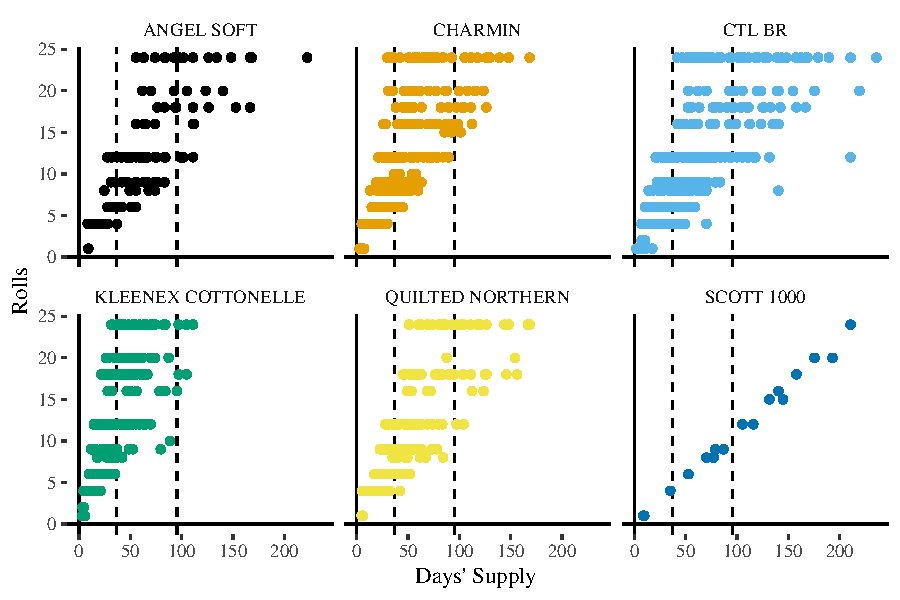
\includegraphics[width = 4.8in, height = 3in]{../5_figures/tpSizeQuantityDistributionAllProdsColor.pdf}
\begin{figurenotes}
Figure plots the package sizes and quantities of the top five toilet paper brands and private-label products. The y-axis represents the number of toilet paper rolls contained in a package while the x-axis represents the number of days a product will last a single person household assuming a consumption rate of 57 two-ply sheets per day (Jaffe 2007). Noise is added vertically to better illustrate the number of products available within package sizes since roll counts are discrete. Dashed lines indicate the 25th and 75th percentiles of the average days' supply purchased by households.
\end{figurenotes}
\begin{figurenotes}[Source]
Nielsen Consumer Panel (2004--2017)
\end{figurenotes}
\label{fig:tpSizeQuantityDistributionAllProds}
\end{figure}

\subsection{Model Setup}
I model a household's purchase decision using a discrete choice framework with random coefficients. When making a purchase, households consider the price, unit price, quality, quantity, and size of each package and choose the package that maximizes their utility. These features are captured in the household $i$'s indirect utility function:
\begin{align}
\label{eq:mlogit}
U_{ijt} = &\beta_{1} Price_{jt} + \beta^i_2 UnitPrice_{jt} + \beta_3 UnitPrice_{jt} \times Reg_{i} +
\\
&\beta^i_4 \log(Days_{j}) + \beta^i_5 BigPack_j + \beta_6 BigPack_j \times House_i +
\nonumber \\
&\beta^i_7 SmallPack_j + \beta_8 SmallPack_j \times House_i + \theta_{b(j)} + \epsilon_{ijt}, \nonumber
\end{align}
where $Price_{jt}$ is the total price of product $j$ at time $t$. $Reg_i$ is an indicator for whether unit price regulations are in effect for household $i$. $Days_j$ is the number of days the package will last (a function of the number of total sheets in the package and the number of people in the household). $UnitPrice_{jt}$ is the per-day, per-person price of the package, since the yield of a package is how many days it will last. $BigPack_j$ is a dummy for the package having more than 12 rolls and $SmallPack_j$ is a dummy for less than 12 rolls.\footnote{Households bunch at 12-roll packages, so this allows for different package preferences around this bunching point.} $House_i$ is an indicator for whether the household lives in a single-family home, with the alternative being an apartment. Finally, $\theta_{b(j)}$ is a brand fixed effect. Brand fixed effects capture quality differences between products. Because households may weigh unit prices or package sizes differently based on unobserved factors, I allow $\beta_2, \beta_4, \beta_5, \beta_7$ to vary. In particular, I assume they are normally distributed and allow for them to be correlated. I assume $\epsilon_{ijt}$ is iid Type 1 extreme value.

This simple model incorporates the key features necessary to quantify the contribution of cognitive and storage costs to the bulk-buying gap. Preferences for package size (a measure of storage costs) are captured by $\beta_5$, $\beta_6$, $\beta_7$, and $\beta_8$, while the effect of displaying per-unit prices is captured by $\beta_3$.

The price coefficient is identified using price variation across shopping trips due to shopping at different stores or sales. The size coefficient is identified by variation in the product ``concentration'' as illustrated in Figure \ref{fig:tpSizeQuantityDistributionAllProds}. That is, given their preferred days' supply (x-value), some households choose large packages and some choose small packages (y-value). I estimate the model using simulated maximum likelihood.\footnote{I use the `mlogit` package which implements Ken Train's Matlab code in R \citep{revelt1998,mlogit}.} To increase accuracy and reduce computational burden, I use pseudo-random Halton draws in the estimation procedure \citep{hensher2003}.

\section{Estimation and Counterfactual Results}
\label{estimation}

I estimate this model separately for each income quartile using household purchases from 2016. I observe about 45,500 toilet paper purchases across about 14,800 households at grocery stores and mass merchandisers.

Table \ref{tab:mlogit2016_Random} reports model estimates for the random coefficients specification. The estimation results show that both the price and unit price coefficients are negative, implying that all else equal, households prefer lower prices. The interaction terms reveal that when unit prices are posted, all households are more sensitive to unit prices. This pattern supports the assertion that households respond to the provision of new price information. All households prefer to have more days' supply of toilet paper compared to less. In terms of storage costs, all households select against large sizes and, with the exception of the highest-income households, this preference is not significantly different based on their housing type. On the other hand, all households also dislike small packages. Under a pure storage costs story, the small packages would have been expected to have a positive sign for low-income households. However, as mentioned in the model specification section, there is bunching at 12-roll packages across households of all types, so this negative sign on the small size is likely a result of that bunching.

\begin{table}[!htbp] \centering
  \caption{Random Coefficient Estimation Results (2016)}
  \label{tab:mlogit2016_Random}
\begin{tabular}{@{\extracolsep{5pt}}lcccc}
\\[-1.8ex]\hline
\hline \\[-1.8ex]
 & $<$25k & 25-50k & 50-100k & $>$100k \\
\\[-1.8ex] & (1) & (2) & (3) & (4)\\
\hline \\[-1.8ex]
 Total Price & $-$0.300$^{***}$ & $-$0.287$^{***}$ & $-$0.284$^{***}$ & $-$0.196$^{***}$ \\
  & (0.011) & (0.007) & (0.006) & (0.009) \\
  Unit Price & $-$4.114$^{***}$ & $-$2.642$^{***}$ & $-$2.969$^{***}$ & $-$3.243$^{***}$ \\
  & (0.290) & (0.124) & (0.105) & (0.155) \\
  . : Reg & $-$1.914$^{***}$ & $-$1.759$^{***}$ & $-$0.819$^{***}$ & $-$0.503$^{***}$ \\
  & (0.330) & (0.161) & (0.123) & (0.149) \\
  Log(Days) & 1.146$^{***}$ & 1.381$^{***}$ & 1.452$^{***}$ & 0.843$^{***}$ \\
  & (0.078) & (0.050) & (0.047) & (0.071) \\
  Large Size & $-$1.654$^{***}$ & $-$1.194$^{***}$ & $-$1.288$^{***}$ & $-$1.104$^{***}$ \\
  & (0.174) & (0.096) & (0.098) & (0.181) \\
  . : Home & 0.273$^{*}$ & 0.101 & $-$0.016 & 0.422$^{**}$ \\
  & (0.147) & (0.097) & (0.093) & (0.179) \\
  Small Size & $-$0.437$^{***}$ & $-$0.345$^{***}$ & $-$0.504$^{***}$ & $-$0.807$^{***}$ \\
  & (0.083) & (0.062) & (0.066) & (0.139) \\
  . : Home & $-$0.173$^{*}$ & $-$0.241$^{***}$ & $-$0.221$^{***}$ & $-$0.202 \\
  & (0.095) & (0.067) & (0.069) & (0.140) \\
 \hline \\[-1.8ex]
   $\sigma_{unitPrice}$ & 6.009$^{***}$ & 4.973$^{***}$ & 4.791$^{***}$ & 3.849$^{***}$ \\
                      & (0.241)      & (0.116)           & (0.092)       & (0.113) \\
     $\sigma_{log(Days)}$ & 1.620$^{***}$ & 1.499$^{***}$ & 1.812$^{***}$ & 1.651$^{***}$ \\
                        & (0.062)       & (0.039)       & (0.035)         & (0.056) \\
     $\sigma_{Large}$ & 1.847$^{***}$ & 1.327$^{***}$ & 1.647$^{***}$ & 1.846$^{***}$ \\
                      & (0.142)         & (0.073)     & (0.065)       & (0.085) \\
     $\sigma_{Small}$ & 2.111$^{***}$ & 2.181$^{***}$ & 2.011$^{***}$ & 2.353$^{***}$ \\
                    & (0.083)         & (0.048)       & (0.042)       & (0.067) \\
 \hline \\[-1.8ex]

Brand FE's & Y & Y & Y & Y \\
Observations & 4,968 & 12,950 & 17,875 & 7,942 \\
Log Likelihood & $-$14,502.240 & $-$37,679.860 & $-$51,245.220 & $-$22,705.370 \\
\hline
\hline \\[-1.8ex]
\end{tabular}
\begin{tablenotes}
Table presents MLE estimates from Equation \ref{eq:mlogit}. ``Total Price'' denotes the total price of the package while ``unit price'' is the price per day that the package will last (assuming constant consumption of 57 sheets per day (Jaffe 2007)). ``Reg'' indicates whether unit price regulations are in effect. ``Large'' indicates packages that are larger than 12 rolls and ``small'' indicates packages that are smaller than 12 rolls. A 12-roll package is the reference group. ``House'' indicates if the household lives in a single-family home (reference group is an apartment). $^{*}$p$<$0.1; $^{**}$p$<$0.05; $^{***}$p$<$0.01
\end{tablenotes}
\begin{tablenotes}[Source]
Nielsen Consumer Panel (2016) and Nielsen Retail Scanner (2016)
\end{tablenotes}
\end{table}


Each of the random coefficients displays substantial heterogeneity.\footnote{Since each random coefficient was assumed to be normally distributed, some households may have a non-intuitive valuation for product attributes, such as a positive valuation for unit price. Sign restrictions can be imposed by assuming alternative distributions, such as a log-normal distribution.} Overall, lower income households exhibit more heterogeneity in their sensitivity to unit prices, as implied by the standard deviations of the unit price coefficient.

Figure \ref{fig:elasticity_Random} plots the distribution of own-price elasticities for each product using the random coefficients estimates. The majority of elasticities fall between -1.7 and -5.1 with poorer households having larger elasticities (in magnitude).\footnote{Table 4 of \citet{cohen2008} reports elasticities ranging from -1.94 to -2.54 for paper towels. My estimates cover this range, but have larger tails.}

\begin{figure}[!htb]
\centering
\caption{Distribution of Price Elasticity by Household Income}
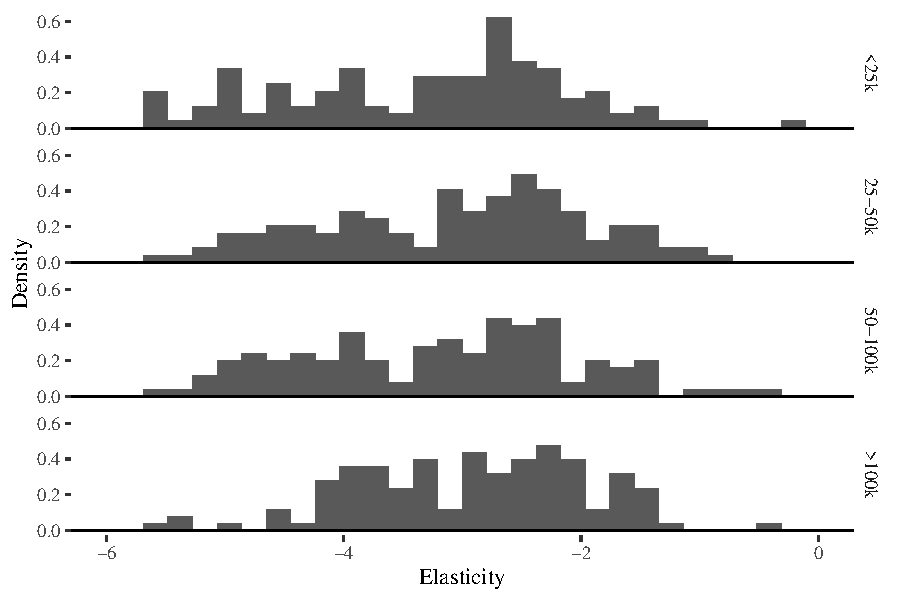
\includegraphics[width = 5in, height = 3in]{../5_figures/elasticity2016_Random.pdf}
\begin{figurenotes}
Figure plots the distribution of price elasticities resulting from the estimation of Equation \ref{eq:mlogit}, using random coefficients.
\end{figurenotes}
\begin{figurenotes}[Source]
Nielsen Consumer Panel (2016) and Nielsen Retail Scanner (2016)
\end{figurenotes}
\label{fig:elasticity_Random}
\end{figure}

\subsection{Model Fit}
I examine model fit by comparing how well the model predicts the average size purchased for each income group. Since coefficients are random, the choice probabilities take the following form:
\begin{equation}
P_{ijt} = \int \frac{e^{\beta' x_{ijt}}}{\sum_j e^{\beta' x_{ijt}}} f(\beta) d\beta,
\end{equation}
I use simulation to approximate the integral by taking 1,000 draws from the joint distribution of $\beta$. Table \ref{tab:modelFit_Random} compares the overall model predictions to the actual data. Overall, the fit is close, but the model over-predicts the amount purchased across all households, primarily because it over-predicts the purchases of particularly large generic packages. For example, a particular generic 12-pack has a 1--2\% share for each income group, but based on its characteristics, the model predicts a 3--5\% share. The model assumes that all generic brands are equal, but in reality, it may be the case that generic brands differ based on the retailer that sells them. This additional dimension of heterogeneity could be captured by more granularly defining brands by the retailer that sells them.

\begin{table}[!htbp] \centering
\caption{Random Coefficient Model Fit (Days' Supply Purchased)}
\label{tab:modelFit_Random}
\begin{tabular}{@{\extracolsep{5pt}}lcc}
\\[-1.8ex]\hline
\hline \\[-1.8ex]
Income & Data & Model \\
\hline \\[-1.8ex]
$<$25k    & 48.64 & 50.67 \\
25-50k  & 49.07 & 52.45 \\
50-100k & 51.23 & 54.48 \\
$>$100k   & 53.85 & 54.93 \\
\hline
\hline \\[-1.8ex]
\end{tabular}
\begin{tablenotes}
Table compares the average days' supply of toilet paper purchased in the data with the predicted purchase from the model. I assume an average daily consumption rate of 57 two-ply sheets per day (Jaffe 2007).
\end{tablenotes}
\begin{tablenotes}[Source]
Nielsen Consumer Panel (2016) and Nielsen Retail Scanner (2016)
\end{tablenotes}
\end{table}


\subsection{Counterfactuals}
\label{counterfactual}

Using the parameter estimates from the previous section, I predict how households respond to lower storage costs and universal unit price regulation. For these counterfactual exercises, I compare all counterfactual results to a ``base case'' of predicted purchases given their current shopping environment. I consider two counterfactual scenarios:

\begin{enumerate}
   \item \textbf{Unit-Price Regulation:} Unit-price regulations are adopted everywhere.
   \item \textbf{Reduced Storage Costs:} All households have the same storage costs (i.e., size preferences) as high-income households.
\end{enumerate}

For the unit-price regulation scenario, I set each household's unit price coefficients equal to the sum of its coefficient and the regulation interaction term. For households making under \$25,000, their unit price coefficient becomes $-4.114 - 1.914 = -6.028$. For the reduced storage cost scenario, I set all size coefficients equal to the coefficients for households making over \$100,000.

Table \ref{tab:counterfactualMNLDays} reports the counterfactual predictions for the random coefficients model.

\begin{table}[!htbp] \centering
\caption{Predicted Effects on Bulk Purchasing}
\label{tab:counterfactualMNLDays}
\begin{tabular}{lccc}
\\[-1.8ex]\hline
\hline \\[-1.8ex]
Income   & Base    & + Unit Price Regs   &  + Rich Storage  \\
\hline
<25k     & 55.03   & 55.94              & 61.61 \\
25-50k   & 53.31   & 54.72              & 57.57 \\
50-100k  & 57.37   & 57.93              & 64.83 \\
>100k    & 57.86   & 57.86              & 57.86 \\
\\[-1.8ex]\hline
\hline \\[-1.8ex]
\end{tabular}
\caption*{Note: This table reports predicted package quantities purchased by households using model estimates of Equation (\ref{eq:mlogit}). Units are number of days the chosen package will last assuming average daily consumption rate of 57 two-ply sheets (Jaffe 2007). The "Unit Price Regs" scenario imposes unit price regulations everywhere. The "Rich Storage" scenario imposes that all households have the same preferences for "large" packages as households making over \$100k. Scenarios are cumulative.}
\end{table}


The random coefficient counterfactuals, while overpredicting the average days' supply purchased, predicts a gap of 4.26 days' supply between high- and low-income households. After universally adopting unit price regulations, all households increase their purchasing, but the gap between high- and low-income households shrinks to 3.16 days' supply. Equalizing storage costs actually reverses the gap with the lowest income households buying 1.03 days' supply more than high-income households. This dramatic increase is driven by the fact that middle- and low-income households continue to be highly price-sensitive and have a stronger preference for large quantities.

These counterfactuals support the main findings from Section \ref{factors} which showed that unit price regulations increase bulk buying and that storage costs are a substantial factor preventing households from buying in bulk. Since the earlier sections examined bulk purchasing across all non-food products, I repeat the earlier analysis on mover households specifically for toilet paper purchases. I estimate a modified version of Equation \ref{eq:unitPriceMove} which replaces share of bulk purchases with log days' supply of toilet paper:
\begin{equation}
\label{eq:unitPriceMoveTP}
Log(DaysSupply)_{it} = \alpha + \beta_1 Reg_{it} + \beta_2 SingleFamily_{it} + \gamma X_{it} + \lambda_i + \lambda_t + \epsilon_{it},
\end{equation}
Table \ref{tab:unitPriceLawMoversTP} shows that households increase the days' supply purchased by 3.5\% when unit prices are posted and by 2.6\% when they move into a single-family home. The model predictions are in line with these changes. The random coefficients model predicts that purchasing increases by 1.6\%--5.3\% when unit prices are posted (compared to 3.5\% above) and by 4.6\%--8.0\% when storage costs are reduced (compared to 2.6\% above). The reduced-form estimates and model predictions line up quite well with regards to posting unit prices. However, there are some differences between the two types of estimates with respect to storage costs. Part of this difference may be because home type (apartment or single-family home) does not capture true storage costs while the random coefficients model offers more flexibility to capture heterogeneity between households even with the same type of housing. For example, the presence of a basement, garage, or even the number of bathrooms may all influence the storage costs for toilet paper, but those are all differences that can exist within single-family homes.

Overall, reducing cognitive costs and increasing the salience of unit prices helps households make better value decisions, and generate a strong boost to bulk buying. Adopting unit price regulations are a relatively straightforward policy approach to encourage bulk buying, especially compared to the challenge of feasibly reducing storage costs for low-income households.


% Table created by stargazer v.5.2.2 by Marek Hlavac, Harvard University. E-mail: hlavac at fas.harvard.edu
% Date and time: Fri, Oct 18, 2019 - 05:04:27 PM
\begin{table}[!htbp] \centering 
  \caption{} 
  \label{} 
\begin{tabular}{@{\extracolsep{5pt}}lcc} 
\\[-1.8ex]\hline 
\hline \\[-1.8ex] 
\\[-1.8ex] & (1) & (2)\\ 
\hline \\[-1.8ex] 
 Regulation & 0.029$^{*}$ & 0.035$^{**}$ \\ 
  & (0.015) & (0.015) \\ 
  Single-Family Home &  & 0.026$^{***}$ \\ 
  &  & (0.006) \\ 
 \hline \\[-1.8ex] 
Household FE & Y & Y \\ 
Year FE & Y & Y \\ 
Demographics & N & Y \\ 
Observations & 4,553,957 & 4,553,957 \\ 
Adjusted R$^{2}$ & 0.507 & 0.508 \\ 
\hline 
\hline \\[-1.8ex] 
\textit{Note:}  & \multicolumn{2}{l}{$^{*}$p$<$0.1; $^{**}$p$<$0.05; $^{***}$p$<$0.01} \\ 
\end{tabular} 
\end{table} 

%
%  Given the model predictions, I can also estimate how the average unit price varies in each counterfactual scenario. Table \ref{tab:counterfactualMNLPrice} reports how the average unit price paid (in cents per day) changes under each counterfactual scenario.
%  \begin{table}[!htbp] \centering
\caption{Predicted Effects on Unit Prices Paid (Cents / Day)}
\label{tab:counterfactualMNLPrice}
\begin{tabular}{lccc}
\\[-1.8ex]\hline
\hline \\[-1.8ex]
Income   & Base    & + Unit Price Regs   &  + Rich Storage  \\
\hline
<25k     & 15.58   & 14.72              & 14.66 \\
25-50k   & 16.49   & 15.19              & 15.11 \\
50-100k  & 16.79   & 16.13              & 16.12 \\
>100k    & 18.30   & 18.30              & 18.30 \\
\\[-1.8ex]\hline
\hline \\[-1.8ex]
\end{tabular}
\caption*{Notes: This table reports predicted unit price (cents / day) paid by households using estimates of Equation (\ref{eq:mlogit}). The "Unit Price Regs" scenario imposes unit price regulations everywhere. The "Rich Storage" scenario imposes that all households have the same preferences for "large" packages as households making over \$100k. Scenarios are cumulative.}
\end{table}

%
%  Household pay a lower unit price under both counterfactual scenarios. Universally displaying unit prices reduces the average unit price paid for the lowest-income households from 21.30 cents to 20.41 cents. Setting storage costs equal to those of high-income households further reduces the average unit price paid to 20.29 cents. Overall, these two policies reduce the average unit price paid by 5\%. Similar reductions are achieved by other households. Overall, posting unit prices and reducing storage costs encourages households, especially the lowest-income households, to buy larger quantities and pay lower unit prices.

\section{Conclusion}
\label{conclusion}

This paper documents the new fact that low-income households are less likely to take advantage of quantity discounts relative to high-income households. This gap is especially large for storable, necessity items like toilet paper and paper towels. If low-income households bought in bulk like high-income households, they could save 5\% on grocery items, saving an aggregate of \$5.4 billion annually. I provide evidence that \textit{cognitive costs}, \textit{store preferences}, \textit{budget constraints}, and \textit{storage costs} contribute to this gap.

By using state-level variation in whether or not retailers have to display unit prices, I find that displaying unit prices reduces cognitive costs and increases bulk buying. Then, I show that \textit{where} a household shops accounts for a large portion of this disparity and that warehouse clubs increase bulk buying, but only for middle- and high-income households. Low-income households are unlikely to shop at warehouse clubs, even if they are nearby. Next, I demonstrate that low-income households slightly decrease bulk buying towards the end of the month, when budgets are tighter. Finally, I show that households increase bulk buying when they move to larger housing, supporting the fact that storage costs also influence the bulk buying decision.

Combining these features into a discrete choice model of toilet paper purchases, I predict how households' bulk purchasing changes if unit-price regulations are adopted universally and if storage costs are reduced. I find that posting unit prices closes the bulk buying gap by 26\% and reducing storage costs completely closes the gap with middle- and low-income households buying larger quantities than high-income households.

This paper is one of the first to focus on consumer's take-up of quantity discounts and explore the factors that contribute to this decision. It provides evidence that \textit{cognitive costs}, \textit{store preferences}, \textit{budget constraints}, and \textit{storage costs} affect a household's bulk buying decision. These differences have substantial financial consequences for the poorest households and are likely to generate systematic underestimates of consumption inequality if quantity discounts offset quality differences between products. Additionally, if the prices of large and small packages evolve differently, then households may experience substantial changes in their buying power. Future work will determine the extent to which inequality and inflation measures are underestimated because of quantity discounts.

% Bibliography
\bibliographystyle{aea}
\bibliography{reference}

\newpage
\appendix

%   ## CPI Products and Weights
%   Table \ref{tab:cpi} shows the CPI weights of storable product categories that often exhibit quantity discounts. These weights come from the Bureau of Labor Statistics Handbook of Methods, Chapter 17: The Consumer Price Index (Updated 2-14-2018). To be conservative in the importance of accounting for quantity discounts, I capture products that are shelf-stable and storable to varying degrees.
%
%   The CPI tries to adjust for quantity discounts in that the "first multiple-unit price is reported for use in the CPI." However, to the extent that there are systematic differences in multi-unit purchases, especially for storable goods, price estimates based on bulk sizes are likely to overestimate the price index for households that consistently buy in bulk and underestimate the price index for households that buy small quantities.
%
%   \textbf{Full CPI Basket:} Includes food and beverages, housing, utilities, apparel, transportation, medical care, recreation, and education.
%
%   \textbf{"Store" Shopping Basket:} This basket is constructed to reflect the set of goods commonly found at grocery/supercenter/general merchandise stores. Includes food and alcohol at home (9.024), household furnishings (3.341), apparel (3.343), pet products (0.659), recreational goods (1.5), and other goods (1.634). I exclude categories such as rent, utilities, energy, transportation, health care, education, and services (including food service).
%
%   \begin{table}[] \centering
  \caption{CPI Basket Shares}
  \label{tab:cpi}
\begin{tabular}{ll}
\textbf{Category}                               & \textbf{Basket Share} \\
\hline
Cereals and cereal products                     & 0.370 \\
Processed fruits and vegetables (excluding frozen) & 0.215 \\
Nonalcoholic beverages and beverage materials   & 0.955 \\
Sugar and sweets                                & 0.299 \\
Fats and oils (excluding butter and margarine)  & 0.168 \\
Other foods (excluding frozen and baby food)    & 1.159 \\
Housekeeping supplies                           & 0.847 \\
Personal care products                          & 0.724 \\
Tobacco and smoking products                    & 0.718 \\
\hline
Total (all CPI)                                 & 5.455 \\
Non-Food Total (all CPI)                        & 2.289 \\
\hline
Share of Store Shopping                         & 27.973 \\
Non-Food Share of Store Shopping                & 11.738 \\
&
  \end{tabular}
\end{table}


\section{Appendix}
\subsection{Data Appendix}
\label{sec:sampleConstruction}

The Nielsen Consumer Panel consists of about 40,000--60,000 US households that provide information on their shopping purchases using in-home scanners or Nielsen's mobile app. Panelists are geographically dispersed and demographically balanced. Households are recruited based on key demographic characteristics, primarily household size, income, age, education, presence of children, race, ethnicity, and occupation. To generate national averages, Nielsen assigns each household a projection factor.

Households are recruited through direct mail and online invitations. To incentivize households to remain in the panel, Nielsen provides monthly prize drawings, sweepstakes, points, and regular communication and support to panelists. Nielsen tries to ensure that incentive methods are non-biasing and regularly tests for its correlation with retention rates. To ensure data quality, Nielsen filters out any households that are poor reporters and do not meet minimum spending thresholds based on their household size. All households in the sample meet this threshold for the full year.

Demographic variables are recorded and updated annually. For my analysis, I collapse some of the demographic variables into more aggregate categories. Household composition measures the number adults and children residing in the home. Marital status is an indicator for whether the head of household is married or not (I do not distinguish between single, divorced, or widowed). Education is an indicator for whether at least one head of household completed college. Housing variables indicate whether a household lives in a single-family home, and apartment, or a mobile home. Finally, age is the age of the head of household. In the case of two heads, I average the two ages.

To construct my analysis sample, I remove any households where the head of household is a student or a member of the military because these households likely have different living arrangements that are not representative of a typical household's decision (i.e., on campus housing or barracks are different than traditional homes and apartments). I drop any households living in mobile homes as well because this type of housing could include a wide range of house types including RVs and manufactured homes. I also remove any households making less that \$5,000 and those that could not be geocoded based on their zip code.\footnote{I use the 2017 Census Gazetteer to assign zip codes to the latitude and longitude of their population-weighted centroid}. Finally, some households were dropped because they could not be matched to tract-level vehicle access data.\footnote{Vehicle access data comes from the 2009--2013 American Community Survey, which asks how individuals get to work. There is limited variation in this measure since most respondents have vehicle access. For context, only 4\% of Nielsen households live in Census tracts less than 90\% access to cars.} Table \ref{tab:homeScanClean} reports how many households were removed based on this cleaning procedure.


% Table created by stargazer v.5.2.2 by Marek Hlavac, Harvard University. E-mail: hlavac at fas.harvard.edu
% Date and time: Thu, Oct 10, 2019 - 08:37:12 AM
\begin{table}[!htbp] \centering 
  \caption{Homescan Sample} 
  \label{tab:homeScanClean} 
\begin{tabular}{@{\extracolsep{5pt}} cc} 
\\[-1.8ex]\hline 
\hline \\[-1.8ex] 
Step & HH \\ 
\hline \\[-1.8ex] 
Starting HH: & $178,232$ \\ 
Exclude military and students: & $175,102$ \\ 
Exclude Households under 5k: & $174,106$ \\ 
Exclude Mobile Homes: & $167,065$ \\ 
Drop ZIPs Not Geocoded: & $166,366$ \\ 
Cannot Be Matched to Car Access: & $166,164$ \\ 
\hline \\[-1.8ex] 
\end{tabular} 
\end{table} 


In the purchase data, I exclude alcohol, tobacco, pet items, health and beauty items, general merchandise, ``magnet,'' and ``deferred'' product categories from my analysis. Alcohol and tobacco are excluded because of their addictive qualities, which may induce peculiar purchase patterns. For example, a smoker may choose to only buy one pack of cigarettes with the intention of quitting even though a full carton may deliver a better value. Pet items are excluded to focus on products intended for human consumption. I exclude health and beauty items and general merchandise because these products such as trash cans, printers, eye shadow, and antacids are unlikely to be bought in bulk or have irregular consumption patterns. ``Deferred'' categories are categories that Nielsen has stopped tracking, so to maintain a consistent sample of products, these are excluded from my analysis. Finally, ``magnet'' purchases are items which do not have a UPC codes such as fresh fruits and vegetables, deli counter items, or bakery items. Because these items are only recorded for a subset of Nielsen households and are not standardized, I also exclude them from my analysis. This process leaves me with 721 unique product categories. Because this paper focuses on bulk purchases, I also exclude 28 categories that have five or fewer sizes across all possible products.\footnote{These excluded categories are: jelled aspic salad, sour cream sauce mix, canned roast beef, canned roast beef hash, retort pouch bags, prepared sandwiches, canned rice, canned dumplings, canned bread, frozen vegetables in pastry, frozen grapefruit juice, frozen grape juice, frozen orange juice, frozen cream substitutes, canned ham patties, bathroom accessory, packaged soap, borateem, dry starch, grease relief, bathroom brushes, miscellaneous brushes, thermometers, dustpans, feather dusters, laundry baskets, sanitary belts, gift package with candy or gum.} Overall, the products analyzed are common household staples including almost all food categories, basic toiletry items, and non-food essentials like toilet paper, soaps/detergents, and diapers. See Table \ref{tab:homeScanProducts} for summary statistics of the top 20 product categories by annual spending.

\begin{table}[!htbp] \centering
  \caption{Summary Statistics of Top 20 Product Categories in Nielsen Homescan Data (2017)}
  \label{tab:homeScanProducts}
\begin{tabularx}{\linewidth}{lXccccc}
\\[-1.8ex]\hline
\hline \\[-1.8ex]
Product & Annual \newline Spending & SD & Avg. Price & SD  & Avg. Size & SD \\
\hline \\[-1.8ex]
Soft Drinks & $79.38$ & $139.02$ & $4.75$ & $4.17$ & $85.87$ & $53.81$ \\
Diet Soft Drinks & $74.82$ & $132.79$ & $4.73$ & $5.07$ & $84.18$ & $65.06$ \\
Milk & $65.65$ & $77.02$ & $3.11$ & $1.79$ & $97.79$ & $35.00$ \\
Cereal & $57.97$ & $68.37$ & $4.06$ & $2.10$ & $18.05$ & $8.17$ \\
Toilet Paper & $56.15$ & $49.47$ & $11.44$ & $7.09$ & $17.09$ & $10.51$ \\
Yogurt & $55.00$ & $75.68$ & $3.28$ & $2.17$ & $17.25$ & $15.22$ \\
Coffee & $53.97$ & $61.69$ & $8.60$ & $5.74$ & $21.84$ & $11.05$ \\
Bread & $50.03$ & $47.09$ & $2.88$ & $1.52$ & $20.54$ & $4.64$ \\
Cookies & $46.97$ & $57.60$ & $3.59$ & $3.44$ & $13.02$ & $6.39$ \\
Fresh Meat & $46.96$ & $62.86$ & $7.75$ & $5.03$ & $30.48$ & $24.97$ \\
Frozen Pizza & $44.48$ & $60.64$ & $5.99$ & $3.67$ & $20.69$ & $12.48$ \\
Bottled Water & $44.06$ & $73.46$ & $4.21$ & $3.75$ & $261.91$ & $181.39$ \\
Fresh Fruit & $42.68$ & $64.91$ & $4.28$ & $2.06$ & $1.93$ & $1.31$ \\
Choc. Candy & $41.05$ & $53.83$ & $3.91$ & $3.67$ & $8.64$ & $9.15$ \\
Detergent & $40.17$ & $45.29$ & $10.05$ & $7.85$ & $99.52$ & $61.23$ \\
Shred. Cheese & $39.16$ & $42.80$ & $4.21$ & $2.45$ & $13.37$ & $10.98$ \\
Bacon & $37.63$ & $45.44$ & $6.87$ & $4.67$ & $17.42$ & $11.88$ \\
Ice Cream & $37.36$ & $50.34$ & $4.43$ & $2.03$ & $46.80$ & $24.47$ \\
Potato Chips & $35.99$ & $41.71$ & $3.04$ & $1.89$ & $8.87$ & $3.81$ \\
Canned Soup & $32.39$ & $38.36$ & $3.21$ & $2.22$ & $22.07$ & $17.33$ \\
\\[-1.8ex]\hline
\hline \\[-1.8ex]
\end{tabularx}
\begin{tablenotes}
Table reports summary statistics for the top 20 product categories by total spending. Annual spending is the average spending in that product category among households that purchased in that product category over the course of the year. Average price and average size are the average prices and sizes of products purchased in their corresponding category. All estimates are weighted using Nielsen's projection weights. Prices are in nominal 2017 dollars. Sizes are reported in common units for for that category (e.g. ounces for milk).
\end{tablenotes}
\begin{tablenotes}[Source]
Nielsen Consumer Panel (2004--2017)
\end{tablenotes}
\end{table}


To compare sizes across different product categories, I assign each product to its quintile in the size distribution for that product category. I assign quintiles based upon the sample quintiles of product sizes to ensure that each quintile has 20\% of available products in its support. An alternative strategy would assign quintiles based on cutting the range of product sizes into equal intervals. However, in some product categories, this risks generating quintiles with sparse support when there is an especially large package available. As an example, consider eggs. Most packages contain 6, 12, or 18 eggs, but there are some products that offer up to 15-dozen eggs (180 eggs). Generating quintiles by cutting the available range into equal intervals would generate quintiles of 1-36, 37-72, 73-108, 109-144, 145-180 which would assign almost all packages to the first quintile and the fifth quintile. Using the sample quintiles generates a more even distribution ensuring better support of each quintile. For products with a narrow range of sizes that fall in multiple quintiles, I assign the product to the minimum quintile. For example, over 60\% of egg products are dozens, which covers three quintiles. I assign all products with 12 or fewer eggs to the first quintile.

\subsection{Quantity Discounts and Coupon Savings}
\label{coupons}
% This uses the discountSavings.R script
% This uses the couponSavings.R script

This section compares savings from quantity discounts to savings from coupons. To be conservative, I compare the savings from redeemed coupons (likely higher than the average savings of all coupons offered) to savings offered by quantity discounts (likely lower than quantity discounts actually redeemed). For each product purchased in the Consumer Panel data, households can input the value saved if they used a coupon. For each product category, I compute the average discount across all products in that category.

I then estimate quantity discount savings based on moving from a product in the second quintile to the fourth quintile of the size distribution. This leaves out small product sizes that may have high unit prices due to convenience (e.g., a 20-oz soda bottle at the checkout counter) and especially large sizes that may not be widely available at all stores. This range covers sizes that households are likely to consider when making their purchase decision.

Figure \ref{fig:couponBulkSavings} plots the distribution of coupon savings and estimated bulk savings for food and non-food products. Coupon savings are narrowly clustered with a median savings of 31\% for non-food products and 33\% for food products. Bulk discounts have lower median savings for non-food and food products of 27\% and 23\%, respectively, but are more widely dispersed, even exceeding 50\% savings for some non-food products.\footnote{Smaller shifts, such as from the second to third quintile or third to fourth quintile generate smaller savings, but still preserve the long right tail primarily for non-food products.} Coupon savings are similar across product categories while there is substantial variation in quantity discounts with non-food products offering higher savings.

\begin{figure}[!htb]
 \centering
 \caption{Estimated Savings from Coupons and Bulk Discounts}
 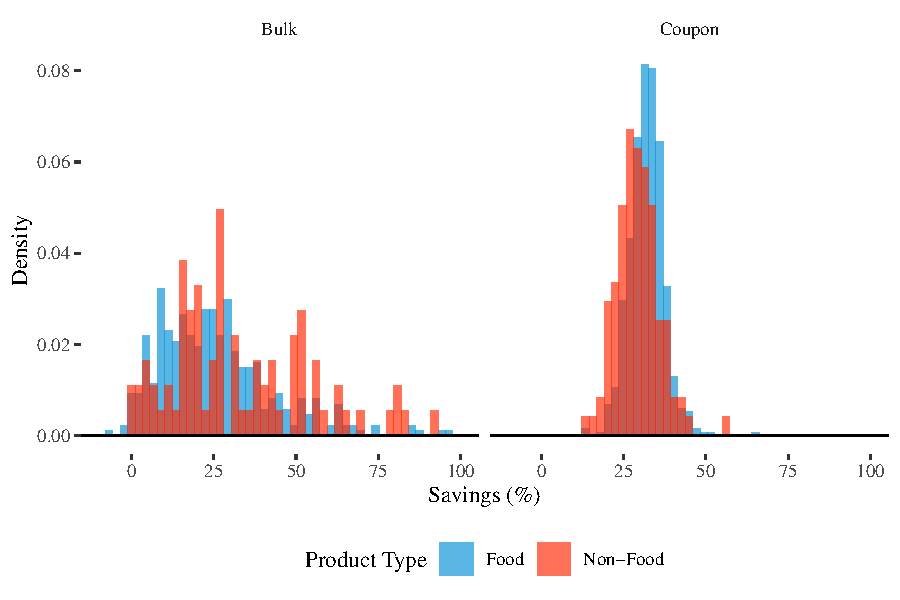
\includegraphics[width = 5in, height = 3in]{../5_figures/couponBulkSavingsColor.pdf}
 \begin{figurenotes}
Figure plots the distribution of savings from coupons and quantity discounts. For each coupon redemption, the percent savings are the ratio of the coupon value to the product's price. These savings are then averaged across all purchases in that product category. Bulk discounts are computed using coefficient estimates obtained from Equation (\ref{eq:bulkDiscount}) relating log unit prices to log package sizes. Bulk savings are the estimated savings obtained from moving from the second to the fourth quintile of the size distribution for each product category.
\end{figurenotes}
\begin{figurenotes}[Source]
Nielsen Consumer Panel (2004--2017) and Nielsen Retail Scanner (2016)
\end{figurenotes}
\label{fig:couponBulkSavings}
\end{figure}

\subsection{Bulk Buying Across Popular Categories}
\label{appendix:bulkGapCategories}

Across popular spending categories, these gaps are particularly large in storable, non-food categories like paper towels and toilet paper, where households making over \$100,000 are more than twice as likely to buy in bulk compared to households making under \$25,000. In popular food categories like milk and eggs, there is little relationship or even a negative relationship between income and bulk buying (See Figure \ref{fig:savingsBehaviorModules}).

\begin{figure}[!htb]
\centering
\caption{Bulk Purchasing by Household Income (Selected Products)}
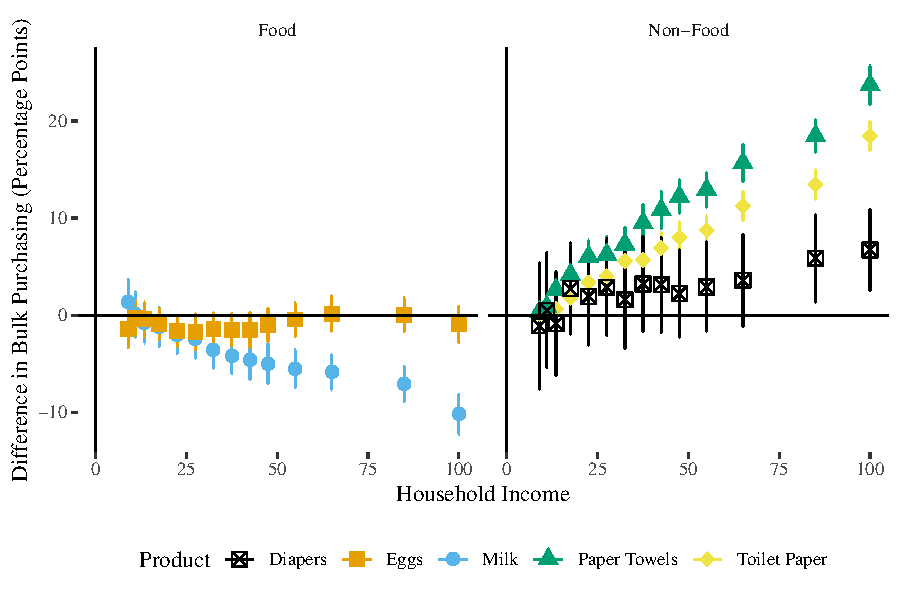
\includegraphics[width = 4.8in, height = 3in]{../5_figures/savingsBehaviorModulesColor.pdf}
\begin{figurenotes}
Figure plots the income bin coefficients from Equation (\ref{eq:discountingBehavior}), which regresses the share of annual purchases that were bulk packages on household characteristics as well as market and year fixed effects. This regression is estimated for milk, eggs, diapers, toilet paper, and paper towels. Nielsen projection weights are used to ensure national representativeness. Households making \$5--\$8k are the reference group. Standard errors are clustered at the DMA level. Coefficient values are reported in Appendix Table \ref{tab:AppendixDiscountingBehaviorMods}
\end{figurenotes}
\begin{figurenotes}[Source]
Nielsen Consumer Panel (2004--2017)
\end{figurenotes}
\label{fig:savingsBehaviorModules}
\end{figure}

\subsection{Alternative Calculation of Missed Quantity Discounts}
\label{excessSpending}
An alternative way of calculating savings from quantity discounts is to calculate first-best savings obtained from purchasing the lowest unit-priced item available, since even high-income households may not be buying at the lowest unit price. I compute this by taking the difference between the unit price paid by each household and the lowest unit price available in the store, given the household's brand preference. I get this information through linking the Nielsen Consumer Panel with the Nielsen Retail Scanner data.

I compute the first-best savings a household could obtain for toilet paper, diapers, milk, and eggs using the following approach. First, for each shopping trip, I compute the lowest unit price the household could have paid given its brand and store choice in that week. The difference in unit prices relative to the unit price chosen is a household's first-best savings for that purchase. Then, to get the average savings for a household, I compute the expenditure-weighted average savings across all purchases for each household. Based on this measure, Table \ref{tab:excessSpending} reports average excess spending by income group, computed for a family of four.

\begin{table}[!htbp] \centering
\caption{Excess Spending by Household Income and Product}
\label{tab:excessSpending}
\begin{tabular}{lcccc}
\\[-1.8ex]\hline
\hline \\[-1.8ex]
            & \multicolumn{2}{c}{Non-Perishable} & \multicolumn{2}{c}{Perishable} \\
              \cline{2-3}                             \cline{4-5}
Income      & Toilet Paper  & Diapers & Milk  & Eggs \\
\hline
<\$25k      & 0.36          & 0.33    & 0.31  & 0.17 \\
\$25-50k    & 0.35          & 0.33    & 0.30  & 0.17 \\
\$50-100k   & 0.34          & 0.33    & 0.31  & 0.17 \\
>\$100k     & 0.33          & 0.31    & 0.33  & 0.18  \\
\\[-1.8ex]\hline
\hline \\[-1.8ex]
\end{tabular}
\caption*{Notes: This table uses 2006--2016 Nielsen Retail Scanner and Consumer Panel data to compute average excess spending relative to the lowest unit price available given a household's brand and store choice. Average excess spending for a family of four is reported above. For example, a household making <\$25k pays unit prices that are 36\% higher than the lowest unit price available.}
\end{table}


Overall, households could save over 30\% by buying in bulk and low-income households could save even more. I estimate the differences in savings between households from the following regression:
\begin{equation}
\label{eq:excessSpending}
Y_{imt} = \alpha + \sum_q \beta^q Income_{imt} + \gamma X_{imt} + \lambda_{mt} + \epsilon_{imt},
\end{equation}
where $Y_{imt}$ is the excess spending of household $i$ in market $m$ in year $t$. $Income_{imt}$ is the household's income bin and $X_{imt}$ consists of household characteristics. $\lambda_{mt}$ is a market-year fixed effect. Table \ref{tab:lowestPrice} shows that low-income households miss out on 1.7--1.8 percentage points more savings than high-income households and the excess spending is primarily in non-food categories like toilet paper (36\% savings) and diapers (33\% savings) as opposed to food categories like milk (31\% savings) and eggs (17\% savings). Given the perishability of food items, these savings may not be realized if the product perishes before it can be consumed.


% Table created by stargazer v.5.2.2 by Marek Hlavac, Harvard University. E-mail: hlavac at fas.harvard.edu
% Date and time: Wed, Jun 19, 2019 - 04:45:00 PM
\begin{table}[!htbp] \centering
  \caption{Regression Results of First-Best Savings Across Household Income and Products}
  \label{tab:lowestPrice}
\begin{tabular}{@{\extracolsep{5pt}}lcccc}
\\[-1.8ex]\hline
\hline \\[-1.8ex]
 & Diapers & Toilet Paper & Eggs & Milk \\
\\[-1.8ex] & (1) & (2) & (3) & (4)\\
\hline \\[-1.8ex]
 25-50k & $-$0.010$^{**}$ & $-$0.005$^{***}$ & 0.001 & $-$0.002 \\
  & (0.005) & (0.001) & (0.001) & (0.001) \\
  50-100k & $-$0.015$^{***}$ & $-$0.013$^{***}$ & 0.004$^{***}$ & 0.002$^{**}$ \\
  & (0.005) & (0.001) & (0.001) & (0.001) \\
  >100k & $-$0.018$^{***}$ & $-$0.017$^{***}$ & 0.018$^{***}$ & 0.010$^{***}$ \\
  & (0.005) & (0.002) & (0.002) & (0.001) \\
 \hline \\[-1.8ex]
Demographics & Y & Y & Y & Y \\
Market-Year FE & Y & Y & Y & Y \\
Observations & 36,903 & 182,415 & 194,413 & 247,451 \\
Adjusted R$^{2}$ & 0.012 & 0.071 & 0.117 & 0.231 \\
\\[-1.8ex]\hline
\hline \\[-1.8ex]
\textit{Note:}  & \multicolumn{4}{l}{$^{*}$p$<$0.1; $^{**}$p$<$0.05; $^{***}$p$<$0.01} \\
\end{tabular}
\caption*{Notes: This table uses 2006--2016 Nielsen Retail Scanner and Consumer Panel data and reports the income coefficients of Equation (\ref{eq:excessSpending}), which regresses savings on household characteristics as well as a market and year fixed effect. Units are percentage points. For example, a household making over \$100k have 2 percentage points lower excess spending than households making under \$25k. Nielsen's projection weights are used for national representativeness.}
\end{table}


Overall, low-income households could benefit substantially from buying in bulk and obtaining lower unit prices. Furthermore, these savings are likely to be more important for low-income households since the marginal utility of an additional dollar of savings is likely to be higher than for high-income households. This analysis also provides evidence that all households could benefit from purchasing at the lowest unit price.

\subsection{Bulk Buying by Store Type or Chain Size}
In this section, I analyze whether the effect of unit pricing differs by store type or chain size. Unit price regulations are only at the state level, but retailers are free to post (or not post) unit prices as long as they are within the boundaries of the law. Large chains may post prices uniformly across all stores in a way that meets the strictest requirements they are subject to. On the other hand, regional chains or independent stores may more closely mirror the laws of the state they are located in. I estimate Equation \ref{eq:unitPrice} using annual household bulk buying at specific stores types or within different chain sizes. Each observation is at the household-year-channel (or chain) level. For example, bulk items accounted for 50\% of Household A's grocery store purchases while bulk items accounted for 100\% of Household A's warehouse club purchases.


% Table created by stargazer v.5.2.2 by Marek Hlavac, Harvard University. E-mail: hlavac at fas.harvard.edu
% Date and time: Thu, Mar 19, 2020 - 05:08:57 PM
\begin{table}[!htbp] \centering 
  \caption{} 
  \label{} 
\begin{tabular}{@{\extracolsep{5pt}}lccccc} 
\\[-1.8ex]\hline 
\hline \\[-1.8ex] 
 & Grocery & Drug & Discount & Dollar & Warehouse \\ 
\\[-1.8ex] & (1) & (2) & (3) & (4) & (5)\\ 
\hline \\[-1.8ex] 
 Vol. Disp & 0.011 & $-$0.011$^{***}$ & $-$0.006 & $-$0.006 & $-$0.004$^{*}$ \\ 
  & (0.009) & (0.003) & (0.005) & (0.005) & (0.002) \\ 
  Mand. Disp & 0.029$^{***}$ & 0.009 & 0.014$^{*}$ & $-$0.022$^{**}$ & 0.010$^{***}$ \\ 
  & (0.005) & (0.007) & (0.008) & (0.010) & (0.003) \\ 
  Mand. Disp, Strict & 0.054$^{***}$ & 0.018$^{***}$ & 0.002 & $-$0.006 & 0.006$^{***}$ \\ 
  & (0.009) & (0.003) & (0.004) & (0.006) & (0.002) \\ 
 \hline \\[-1.8ex] 
Avg Bulk & 0.36 & 0.29 & 0.49 & 0.35 & 0.95 \\ 
Demographics & Y & Y & Y & Y & Y \\ 
Omit California & Y & Y & Y & Y & Y \\ 
Observations & 618,029 & 298,166 & 562,749 & 328,607 & 267,759 \\ 
Adjusted R$^{2}$ & 0.011 & 0.003 & 0.005 & 0.002 & 0.001 \\ 
\hline 
\hline \\[-1.8ex] 
\textit{Note:}  & \multicolumn{5}{l}{$^{*}$p$<$0.1; $^{**}$p$<$0.05; $^{***}$p$<$0.01} \\ 
\end{tabular} 
\end{table} 


Table \ref{tab:unitPriceLawChannel} shows that in the cross-section, stricter unit price regulations are associated with more bulk buying primarily for grocery stores, drug stores, and warehouse clubs. Households in states with strict unit price regulations buy in bulk five percentage points more at grocery stores compared to households in states without any pricing regulations. Since grocery stores tend to be regional or independent, the large positive relationship provides strong evidence that unit price regulations can increase bulk purchasing. Grocery stores also have the richest variety in Nielsen's data with over 900 unique retailers being captured compared to 65 drug stores, 25 discount stores, 17 dollar stores, and 10 warehouse clubs.\footnote{Nielsen's categorization includes a ``catch-all'' category that is not unique to a particular retailer, so it actually uniquely captures 64 drug stores and purchases at other drug stores are assigned to the last ``catch-all'' drug store. Generally, larger retailers are uniquely tracked and smaller ones may fall into the ``catch-all'' category.} Other store types exhibit smaller or insignificant effects, which could be because these are generally large chains that have more uniform pricing practices across all locations.


% Table created by stargazer v.5.2.2 by Marek Hlavac, Harvard University. E-mail: hlavac at fas.harvard.edu
% Date and time: Sat, Mar 21, 2020 - 03:42:59 PM
\begin{table}[!htbp] \centering
  \caption{}
  \label{tab:unitPriceLawChain}
\begin{tabular}{@{\extracolsep{5pt}}lccc}
\\[-1.8ex]\hline
\hline \\[-1.8ex]
 & Local & Regional & National \\
\\[-1.8ex] & (1) & (2) & (3)\\
\hline \\[-1.8ex]
 Vol. Disp & 0.063$^{***}$ & 0.030 & 0.010 \\
  & (0.022) & (0.025) & (0.009) \\
  Mand. Disp & $-$0.067 & $-$0.018 & 0.039$^{***}$ \\
  & (0.053) & (0.014) & (0.009) \\
  Mand. Disp, Strict & 0.064$^{***}$ & 0.070$^{***}$ & 0.026$^{***}$ \\
  & (0.016) & (0.014) & (0.006) \\
 \hline \\[-1.8ex]
Avg Bulk & 0.33 & 0.32 & 0.49 \\
Demographics & Y & Y & Y \\
Omit California & Y & Y & Y \\
Observations & 1,578 & 43,756 & 668,566 \\
Adjusted R$^{2}$ & 0.008 & 0.005 & 0.037 \\
\hline
\hline \\[-1.8ex]
\textit{Note:}  & \multicolumn{3}{l}{$^{*}$p$<$0.1; $^{**}$p$<$0.05; $^{***}$p$<$0.01} \\
\end{tabular}
\end{table}


Table \ref{tab:unitPriceLawChain} shows the results by chain size. Following \citet{jarmin2009}, I define a ``local'' chain as only having locations in one state, a ``regional'' chain has locations in two to ten states, and a ``national'' chain has locations in more than ten states. In the cross-section, stricter unit price regulations are associated with more bulk buying across all chain types. The effect is strongest for local and regional chains, exhibiting a six to seven percentage point increase in bulk buying relative to states without unit price regulations. National chains still have significant differences, but they are a more moderate three to four percentage point difference relative to states without regulations. Overall, the relative effect is strongest for the smaller chains that are likely to only be subject to a limited set of regulations and the effect is weaker for national chains which may be more likely to adopt pricing practices that satisfy the strictest requirements nationwide.

\subsection{Annual Consumption Analysis}
\label{lasso}
I show that income is not predictive of a household's toilet paper consumption rate first using basic OLS regressions. I then formalize the result using a 100-fold cross-validated elastic net regression to select the most predictive variables. If income and toilet paper consumption are related, then an OLS regression will extract the correlation.

First, I compute a household's daily consumption by aggregating the total number of sheets purchased by a household in a given year, excluding the final purchase of the year since it may not be consumed within the year. I divide this total by the number of days between the first and last purchase of the year to get a household's average daily consumption rate. This method avoids complications where end of the year inventory may be carried over to the following year or a household may start the year with some inventory.

Given a household's average daily consumption rate, I estimate an OLS regression of consumption on household characteristics:
\begin{equation}
\label{eq:annualConsumption}
Y_i = \alpha + \beta X_i + \epsilon_i,
\end{equation}
where $Y_i$ is household $i$'s average daily consumption and $X_i$ is a vector of household characteristics. Figure \ref{fig:annualPurchasesTP} plots the income coefficients of an OLS regression including only income covariates and the coefficients when household characteristics are included. The graph illustrates that after controlling for covariates that plausibly cause increased consumption, income is not significantly correlated with consumption.

\begin{figure}[!htb]
\centering
\caption{Average Daily Consumption by Household Income}
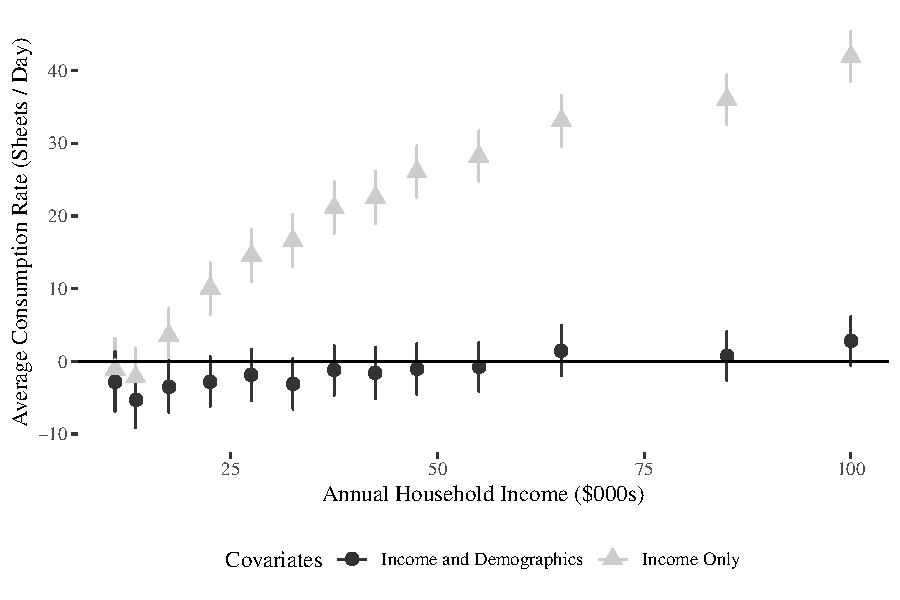
\includegraphics[width = 5in, height = 3in]{../5_figures/annualPurchasesTP.pdf}
\begin{figurenotes}
Figure plots the income bin coefficients from Equation (\ref{eq:annualConsumption}), which regresses average daily household toilet paper consumption on household characteristics. Average daily consumption is computed by dividing total quantity purchased in a year by the number of days a household was active in the panel.
\end{figurenotes}
\begin{figurenotes}[Source]
Nielsen Consumer Panel (2004--2017)
\end{figurenotes}
\label{fig:annualPurchasesTP}
\end{figure}

The above specification omits many other possible covariates that could be correlated with average daily consumption. When there are many possible variables that can be included, there is a risk of over-fitting. Elastic net regularization is a machine learning method that penalizes over-fitting and selects only the most predictive variables.

The elastic net solves the following minimization problem:
\begin{equation}
\min_{\beta} \Vert y - X \beta \Vert^2 + \lambda \left(\alpha \Vert \beta \Vert_1 + (1 - \alpha) \Vert \beta \Vert^2_2 \right),
\end{equation}
where $\Vert \cdot \Vert_1$ is the L1 norm and $\Vert \cdot \Vert_2$ is the L2 norm. The OLS estimate is the $\beta$ that solves the minimization problem with only the first term. The second term and third term provide penalties to shrink and select for the most predictive variables.

I set the mixing parameter $\alpha$ to be 0.5. When covariates are correlated in groups, lasso regression ($\alpha = 1$) tends to only select one and discard all other members of the group while ridge regression ($\alpha = 0$) tends to shrink correlated coefficients towards each other \citep{zou2005}. Because some of the possible covariates form natural groups (e.g., all income bins or all markets), I chose $\alpha = 0.5$ since this tends to include or exclude groups together.

I estimate a 100-fold cross-validated elastic net regression to select the most predictive covariates. The resulting estimates selects many household characteristics including household composition, age, marital status, and race, but excludes almost all income and geographic coefficients.\footnote{Elastic net results are available upon request.}

% # Toilet Paper "Concentration"
% To provide more detail on why toilet paper has different "concentrations," this section provides the geometric intuition.
%
%  Recall that "concentration" refers to the amount of product per unit volume. Therefore, in the case of toilet paper, this will be the ratio of the length of the paper to the volume of the roll. Therefore, to calculate concentration, two values must be computed.
%
%  First, the volume is straightforward since a roll of toilet paper can be modeled as a cylinder. Therefore, the formula for volume is simply $\pi r^2 h$. Computing the length of unspooled toilet paper is more complicated.
%
%  A toilet paper roll can be modeled as an Archimedean spiral (i.e., arithmetic spiral), which has the following polar representation:
%  \begin{equation*}
%  r = a + b \theta,
%  \end{equation*}
%  where $a$ is the starting point of the spiral (distance from the origin) and $b$ is the distance between successive turns of the spiral.
%
%  Given this representation, the length of the spiral takes the following form:
%  \begin{equation*}
%  L = \int_a^b \sqrt((a + b\theta)^2 + b^2) d\theta
%  \end{equation*}
%
%  While this formula has a closed form, it is easier to numerically integrate to get the length of the spiral.
%
%  A cardboard toilet paper tube has an inner radius of about 0.8 inches (this is $a$) and a sheet of toilet paper is about 4.5 inches tall (this is $h$). Additionally, I assume toilet paper has a thickness of 0.01 inches (this is $b$). With these values, I can then compute the concentrations of various rolls of toilet paper. For illustration, I will compute this for rolls ranging from 50 turns to 150 turns (only Concentration column is rounded to two decimal places).
%
%  | Turns | Length | Volume | Concentration |
%  |-------|---------|--------------|---------------|
%  | 50 | 744.816 | 7.605 \pi | 31.17 |
%  | 75 | 1487.33 | 10.81125 \pi | 43.79 |
%  | 100 | 2476.59 | 14.58 \pi | 54.07 |
%  | 125 | 3712.58 | 18.91125 \pi | 62.49 |
%  | 150 | 5195.32 | 23.805 \pi | 69.47 |
%
%  The key takeaways are that concentration is changing as the roll gets bigger. To get a better intuition, compare the 100-turn spiral with the 150-turn spiral. The length has more than doubled (~110\% increase) while the volume has only increased by 60\%. In reality, the ratios are actually much larger because toilet paper is compressible, which means that manufacturers can wind the paper more tightly and are able to achieve large increases in length with negligible changes in volume. Figure \ref{fig:scott} shows that this compressability has even been advertised going back at least 100 years.
%
%  \begin{figure}[!htb]
%  \centering
%  \caption{Scott Toilet Paper Ad from 1915}
%  
\includegraphics[height = 0.4\textwidth]{../5_figures/Scott_ad_1915.png}
%  \label{fig:scott}
%  \end{figure}
%
%  A brief empirical study undertaken by the author found that between two 12-roll packages of Quilted Northern and Angel Soft, a 60\% difference in the number of sheets corresponded to an 8\% difference in physical volume.
%
%  # Bulk-Buying Gaps Across Product Categories
%  \label{discountingAll}
%  To supplement the analysis in Section \ref{bulkPurchasing}, this section provides a comprehensive analysis of bulk purchasing across all product categories. The main paper classified each product as a "bulk" size or not in order to aggregate purchasing across diverse product categories. In this section, I estimate a modified form of Equation \ref{eq:discountingBehavior} which regresses log average package size on income and other demographics. Since I estimate this regression for each of the hundreds of product categories, using log package size provides a more informative view of the difference in purchasing behavior between different household types.
%
%  For each household, I compute the total volume and number of packages purchased over the year for each product category. Dividing the total volume by the number of packages gives the average package size purchased by that household. For example, if a household purchased 20 rolls of toilet paper across two packages, then the average package size purchased is 10 rolls per package. Therefore, I have the average package size purchased for each household-year-product category. To establish that high income is associated with larger average packages, I estimate the following regression for each product category:
%  \begin{equation}
%  \label{eq:bulkBuyingGap}
%  log(Y)_{imt} = \beta_1 Income_{imt} + \beta_2 X_{imt} + \lambda_{m} + \lambda_t + \epsilon_{imt},
%  \end{equation}
%  where $Y$ is the average package size purchased by household $i$ in market $m$ in year $t$. I define a market as a DMA.\footnote{DMAs are non-overlapping groups of counties that define television markets, but they also provide reasonable sub-MSA geographic regions for analysis.} $Income$ is the household's income bin. $X$ controls for other household demographics including household composition, age, marital status, and education. Finally, to capture changes over time within geographic regions, I include a market and year fixed effects $\lambda$.
%
%  Each product category gives a set of coefficients. These coefficients are plotted in Figure \ref{fig:discountingBehaviorChannelAll}. For clarity, I only show product categories in which at least 5000 households made a purchase in a year (about 5--10\% of Nielsen households). The figure shows that there are wide differences in average package sizes purchased across a wide variety of products. For paper towels, aluminum foil, and kitchen trash bags, households making over \$100,000 buy 35\% larger packages than those purchased by households making under \$25,000. Furthermore, the differences between income groups are statistically significant. Households making over \$100,000 purchase larger packages than those making \$50--100,000 who in turn purchase larger packages than those making \$25--50,000.
%
%  In about 60\% of products, higher income households purchase larger packages.
%
%  \begin{figure}[!htb]
%  \centering
%  \caption{Bulk Purchasing Across Product Categories and Income Groups}
%  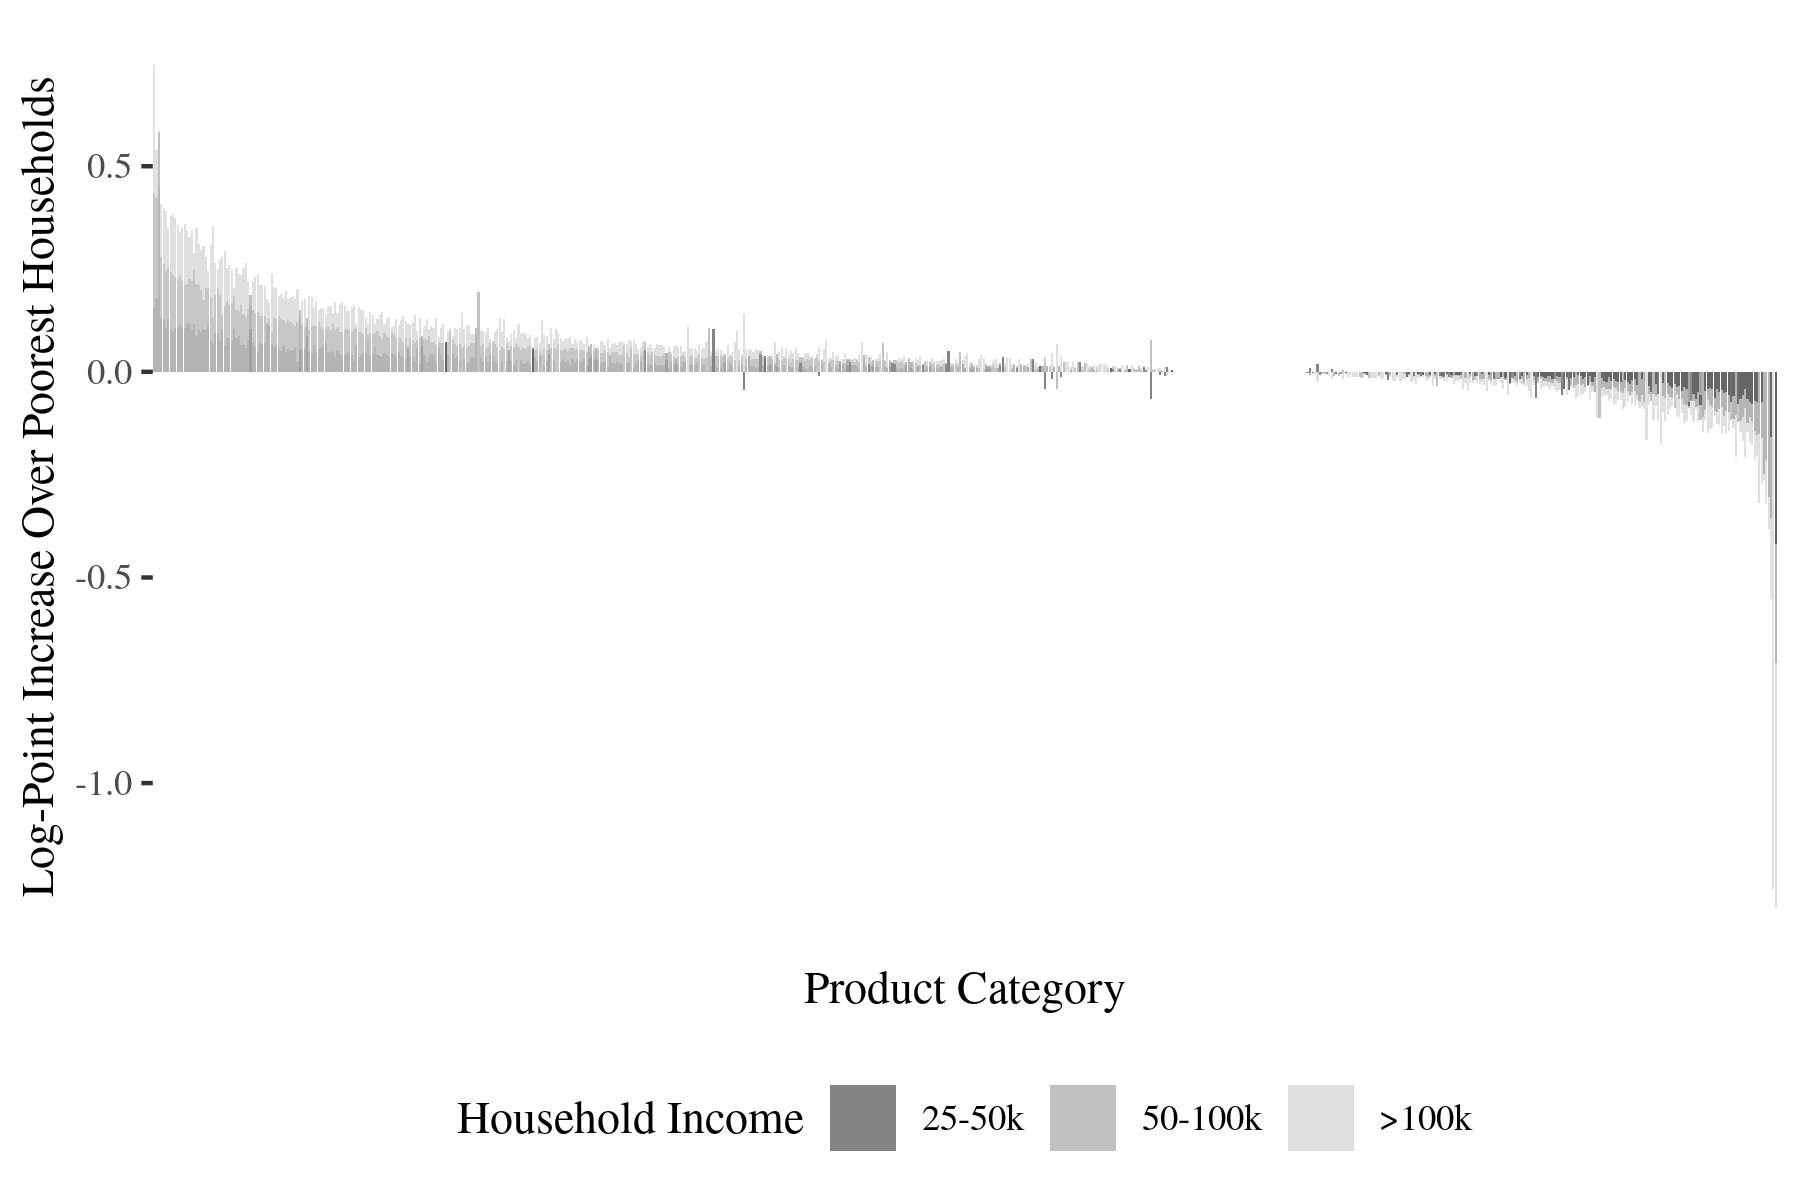
\includegraphics[height = 0.4\textwidth]{../5_figures/discountingBehaviorChannelAll.png}
%  \caption*{Note: Using 2004--2017 Nielsen Consumer Panel data, this figure plots the income coefficients from Equation (\ref{eq:bulkBuyingGap}) which regresses the log average package size purchased on household income, size, age, presence of children, marital status, and education as well as market and year fixed effects. Each bar represents a different product category and only statistically significant coefficients (at the 5\% level) are plotted. Values are relative to households making <\$25,000 (the reference category). Only categories for which more than 5000 households made a purchase in a given year are plotted.}
%  \label{fig:discountingBehaviorChannelAll}
%  \end{figure}

\subsection{Appendix Tables}

% Table created by stargazer v.5.2.2 by Marek Hlavac, Harvard University. E-mail: hlavac at fas.harvard.edu
% Date and time: Thu, Oct 10, 2019 - 09:15:24 AM
\begin{table}[!htbp] \centering 
  \caption{Correlation of Bulk Buying and Demographics (Food Products)} 
  \label{tab:discountingBehaviorFood} 
\begin{tabular}{@{\extracolsep{5pt}}lccccccccc} 
\\[-1.8ex]\hline 
\hline \\[-1.8ex] 
\\[-1.8ex] & (1) & (2) & (3) & (4) & (5) & (6) & (7) & (8) & (9)\\ 
\hline \\[-1.8ex] 
 8-10k & $-$0.005$^{***}$ & $-$0.004$^{**}$ & $-$0.004$^{**}$ & $-$0.003$^{*}$ & $-$0.002 & $-$0.002 & $-$0.002 & $-$0.004$^{**}$ & $-$0.003 \\ 
  & (0.002) & (0.002) & (0.002) & (0.002) & (0.002) & (0.002) & (0.002) & (0.002) & (0.002) \\ 
  10-12k & $-$0.004$^{**}$ & $-$0.005$^{***}$ & $-$0.004$^{**}$ & $-$0.006$^{***}$ & $-$0.006$^{***}$ & $-$0.006$^{***}$ & $-$0.006$^{***}$ & $-$0.008$^{***}$ & $-$0.008$^{***}$ \\ 
  & (0.002) & (0.002) & (0.002) & (0.002) & (0.002) & (0.002) & (0.002) & (0.002) & (0.002) \\ 
  12-15k & $-$0.0001 & $-$0.002 & $-$0.001 & $-$0.002 & $-$0.004$^{**}$ & $-$0.005$^{***}$ & $-$0.005$^{***}$ & $-$0.005$^{***}$ & $-$0.004$^{***}$ \\ 
  & (0.002) & (0.002) & (0.002) & (0.002) & (0.002) & (0.002) & (0.002) & (0.002) & (0.002) \\ 
  15-20k & 0.001 & $-$0.003$^{*}$ & $-$0.002 & $-$0.004$^{***}$ & $-$0.006$^{***}$ & $-$0.006$^{***}$ & $-$0.006$^{***}$ & $-$0.006$^{***}$ & $-$0.005$^{***}$ \\ 
  & (0.002) & (0.002) & (0.002) & (0.002) & (0.002) & (0.002) & (0.002) & (0.001) & (0.001) \\ 
  20-25k & 0.007$^{***}$ & 0.0003 & 0.001 & $-$0.002 & $-$0.005$^{***}$ & $-$0.006$^{***}$ & $-$0.005$^{***}$ & $-$0.006$^{***}$ & $-$0.005$^{***}$ \\ 
  & (0.002) & (0.002) & (0.002) & (0.001) & (0.001) & (0.001) & (0.001) & (0.001) & (0.001) \\ 
  25-30k & 0.013$^{***}$ & 0.004$^{***}$ & 0.004$^{***}$ & $-$0.0002 & $-$0.004$^{***}$ & $-$0.005$^{***}$ & $-$0.004$^{***}$ & $-$0.004$^{***}$ & $-$0.004$^{**}$ \\ 
  & (0.002) & (0.002) & (0.002) & (0.002) & (0.002) & (0.002) & (0.002) & (0.002) & (0.001) \\ 
  30-35k & 0.016$^{***}$ & 0.005$^{***}$ & 0.005$^{***}$ & 0.0004 & $-$0.004$^{**}$ & $-$0.004$^{***}$ & $-$0.003$^{**}$ & $-$0.004$^{**}$ & $-$0.003$^{*}$ \\ 
  & (0.002) & (0.002) & (0.002) & (0.002) & (0.002) & (0.002) & (0.002) & (0.001) & (0.001) \\ 
  35-40k & 0.021$^{***}$ & 0.008$^{***}$ & 0.008$^{***}$ & 0.003$^{**}$ & $-$0.002 & $-$0.002 & $-$0.001 & $-$0.001 & $-$0.0005 \\ 
  & (0.002) & (0.002) & (0.002) & (0.002) & (0.002) & (0.002) & (0.002) & (0.002) & (0.002) \\ 
  40-45k & 0.024$^{***}$ & 0.010$^{***}$ & 0.009$^{***}$ & 0.004$^{***}$ & $-$0.001 & $-$0.001 & 0.0002 & 0.0002 & 0.001 \\ 
  & (0.002) & (0.002) & (0.002) & (0.002) & (0.002) & (0.002) & (0.002) & (0.002) & (0.002) \\ 
  45-50k & 0.028$^{***}$ & 0.011$^{***}$ & 0.011$^{***}$ & 0.005$^{***}$ & $-$0.0001 & $-$0.0003 & 0.001 & 0.001 & 0.002 \\ 
  & (0.002) & (0.002) & (0.002) & (0.002) & (0.002) & (0.002) & (0.002) & (0.002) & (0.002) \\ 
  50-60k & 0.029$^{***}$ & 0.011$^{***}$ & 0.010$^{***}$ & 0.005$^{***}$ & $-$0.001 & $-$0.001 & 0.001 & 0.001 & 0.002 \\ 
  & (0.001) & (0.001) & (0.001) & (0.001) & (0.001) & (0.001) & (0.001) & (0.001) & (0.001) \\ 
  60-70k & 0.035$^{***}$ & 0.015$^{***}$ & 0.014$^{***}$ & 0.008$^{***}$ & 0.002 & 0.001 & 0.003$^{**}$ & 0.004$^{**}$ & 0.004$^{***}$ \\ 
  & (0.002) & (0.002) & (0.002) & (0.002) & (0.002) & (0.001) & (0.002) & (0.001) & (0.001) \\ 
  70-100k & 0.038$^{***}$ & 0.015$^{***}$ & 0.015$^{***}$ & 0.009$^{***}$ & 0.002 & 0.002 & 0.005$^{***}$ & 0.005$^{***}$ & 0.006$^{***}$ \\ 
  & (0.001) & (0.001) & (0.001) & (0.001) & (0.001) & (0.001) & (0.001) & (0.001) & (0.001) \\ 
  >100k & 0.041$^{***}$ & 0.015$^{***}$ & 0.015$^{***}$ & 0.010$^{***}$ & 0.002 & 0.003$^{*}$ & 0.006$^{***}$ & 0.007$^{***}$ & 0.008$^{***}$ \\ 
  & (0.001) & (0.001) & (0.001) & (0.001) & (0.001) & (0.001) & (0.001) & (0.001) & (0.001) \\ 
  Married &  & 0.043$^{***}$ & 0.042$^{***}$ & 0.022$^{***}$ & 0.018$^{***}$ & 0.016$^{***}$ & 0.016$^{***}$ & 0.017$^{***}$ & 0.018$^{***}$ \\ 
  &  & (0.0004) & (0.0004) & (0.0004) & (0.0004) & (0.0004) & (0.0004) & (0.0004) & (0.0004) \\ 
  Age &  &  & $-$0.0002$^{***}$ & 0.0002$^{***}$ & 0.00005$^{***}$ & 0.0001$^{***}$ & 0.00003$^{**}$ & 0.0001$^{***}$ & 0.0001$^{***}$ \\ 
  &  &  & (0.00001) & (0.00001) & (0.00001) & (0.00001) & (0.00001) & (0.00001) & (0.00001) \\ 
  Adults &  &  &  & 0.017$^{***}$ & 0.016$^{***}$ & 0.017$^{***}$ & 0.016$^{***}$ & 0.015$^{***}$ & 0.015$^{***}$ \\ 
  &  &  &  & (0.0002) & (0.0002) & (0.0002) & (0.0002) & (0.0002) & (0.0002) \\ 
  Children &  &  &  & 0.016$^{***}$ & 0.015$^{***}$ & 0.015$^{***}$ & 0.015$^{***}$ & 0.014$^{***}$ & 0.014$^{***}$ \\ 
  &  &  &  & (0.0002) & (0.0002) & (0.0002) & (0.0002) & (0.0002) & (0.0002) \\ 
  Single-Family Home &  &  &  &  & 0.033$^{***}$ & 0.026$^{***}$ & 0.026$^{***}$ & 0.025$^{***}$ & 0.025$^{***}$ \\ 
  &  &  &  &  & (0.0004) & (0.0004) & (0.0004) & (0.0004) & (0.0004) \\ 
  % Car Access &  &  &  &  &  & 0.110$^{***}$ & 0.109$^{***}$ & 0.061$^{***}$ & 0.062$^{***}$ \\ 
  &  &  &  &  &  & (0.002) & (0.002) & (0.002) & (0.002) \\ 
  College &  &  &  &  &  &  & $-$0.006$^{***}$ & $-$0.006$^{***}$ & $-$0.006$^{***}$ \\ 
  &  &  &  &  &  &  & (0.0004) & (0.0004) & (0.0004) \\ 
 \hline \\[-1.8ex] 
Market FE's & N & N & N & N & N & N & N & Y & Y \\ 
Year FE's & N & N & N & N & N & N & N & N & Y \\ 
Observations & 733,894 & 733,894 & 733,894 & 733,894 & 733,894 & 733,894 & 733,894 & 733,894 & 733,894 \\ 
Adjusted R$^{2}$ & 0.011 & 0.030 & 0.030 & 0.050 & 0.058 & 0.062 & 0.062 & 0.101 & 0.102 \\ 
\hline 
\hline \\[-1.8ex] 
\textit{Note:}  & \multicolumn{9}{l}{$^{*}$p$<$0.1; $^{**}$p$<$0.05; $^{***}$p$<$0.01} \\ 
 & \multicolumn{9}{l}{Source: Author calulations from Nielsen Consumer Panel.} \\ 
\end{tabular} 
\end{table} 


% Table created by stargazer v.5.2.2 by Marek Hlavac, Harvard University. E-mail: hlavac at fas.harvard.edu
% Date and time: Tue, Aug 20, 2019 - 02:00:25 PM
\begin{table}[!htbp] \centering
  \caption{Correlation of Bulk Buying and Demographics (Non-Food Products)}
  \label{tab:discountingBehaviorNonFood}
  \resizebox{0.95\textwidth}{!}{
\begin{tabular}{@{\extracolsep{5pt}}lccccccc}
\\[-1.8ex]\hline
\hline \\[-1.8ex]
\\[-1.8ex] & (1) & (2) & (3) & (4) & (5) & (6) & (7)\\
\hline \\[-1.8ex]
 8-10k & 0.008$^{***}$ & 0.008$^{***}$ & 0.008$^{***}$ & 0.008$^{***}$ & 0.008$^{***}$ & 0.005 & 0.002 \\
  & (0.003) & (0.003) & (0.003) & (0.003) & (0.003) & (0.007) & (0.007) \\
  10-12k & 0.022$^{***}$ & 0.022$^{***}$ & 0.021$^{***}$ & 0.020$^{***}$ & 0.020$^{***}$ & 0.016$^{**}$ & 0.013$^{*}$ \\
  & (0.003) & (0.003) & (0.003) & (0.003) & (0.003) & (0.008) & (0.007) \\
  12-15k & 0.024$^{***}$ & 0.022$^{***}$ & 0.021$^{***}$ & 0.020$^{***}$ & 0.020$^{***}$ & 0.019$^{***}$ & 0.016$^{***}$ \\
  & (0.002) & (0.002) & (0.002) & (0.002) & (0.002) & (0.006) & (0.006) \\
  15-20k & 0.033$^{***}$ & 0.030$^{***}$ & 0.029$^{***}$ & 0.027$^{***}$ & 0.026$^{***}$ & 0.024$^{***}$ & 0.021$^{***}$ \\
  & (0.002) & (0.002) & (0.002) & (0.002) & (0.002) & (0.006) & (0.006) \\
  20-25k & 0.050$^{***}$ & 0.044$^{***}$ & 0.043$^{***}$ & 0.041$^{***}$ & 0.040$^{***}$ & 0.037$^{***}$ & 0.034$^{***}$ \\
  & (0.002) & (0.002) & (0.002) & (0.002) & (0.002) & (0.005) & (0.005) \\
  25-30k & 0.055$^{***}$ & 0.047$^{***}$ & 0.047$^{***}$ & 0.043$^{***}$ & 0.042$^{***}$ & 0.039$^{***}$ & 0.037$^{***}$ \\
  & (0.002) & (0.002) & (0.002) & (0.002) & (0.002) & (0.005) & (0.005) \\
  30-35k & 0.069$^{***}$ & 0.060$^{***}$ & 0.060$^{***}$ & 0.056$^{***}$ & 0.054$^{***}$ & 0.050$^{***}$ & 0.048$^{***}$ \\
  & (0.002) & (0.002) & (0.002) & (0.002) & (0.002) & (0.005) & (0.005) \\
  35-40k & 0.075$^{***}$ & 0.065$^{***}$ & 0.065$^{***}$ & 0.061$^{***}$ & 0.058$^{***}$ & 0.054$^{***}$ & 0.052$^{***}$ \\
  & (0.002) & (0.002) & (0.002) & (0.002) & (0.002) & (0.006) & (0.006) \\
  40-45k & 0.083$^{***}$ & 0.072$^{***}$ & 0.072$^{***}$ & 0.068$^{***}$ & 0.064$^{***}$ & 0.060$^{***}$ & 0.058$^{***}$ \\
  & (0.002) & (0.002) & (0.002) & (0.002) & (0.002) & (0.006) & (0.006) \\
  45-50k & 0.093$^{***}$ & 0.080$^{***}$ & 0.080$^{***}$ & 0.075$^{***}$ & 0.071$^{***}$ & 0.066$^{***}$ & 0.063$^{***}$ \\
  & (0.002) & (0.002) & (0.002) & (0.002) & (0.002) & (0.005) & (0.005) \\
  50-60k & 0.099$^{***}$ & 0.085$^{***}$ & 0.085$^{***}$ & 0.080$^{***}$ & 0.075$^{***}$ & 0.071$^{***}$ & 0.068$^{***}$ \\
  & (0.002) & (0.002) & (0.002) & (0.002) & (0.002) & (0.005) & (0.005) \\
  60-70k & 0.116$^{***}$ & 0.101$^{***}$ & 0.101$^{***}$ & 0.096$^{***}$ & 0.090$^{***}$ & 0.084$^{***}$ & 0.080$^{***}$ \\
  & (0.002) & (0.002) & (0.002) & (0.002) & (0.002) & (0.005) & (0.005) \\
  70-100k & 0.136$^{***}$ & 0.118$^{***}$ & 0.119$^{***}$ & 0.113$^{***}$ & 0.105$^{***}$ & 0.098$^{***}$ & 0.096$^{***}$ \\
  & (0.002) & (0.002) & (0.002) & (0.002) & (0.002) & (0.006) & (0.006) \\
  >100k & 0.172$^{***}$ & 0.152$^{***}$ & 0.152$^{***}$ & 0.146$^{***}$ & 0.135$^{***}$ & 0.123$^{***}$ & 0.115$^{***}$ \\
  & (0.002) & (0.002) & (0.002) & (0.002) & (0.002) & (0.006) & (0.006) \\
  Married &  & 0.033$^{***}$ & 0.034$^{***}$ & 0.022$^{***}$ & 0.024$^{***}$ & 0.029$^{***}$ & 0.028$^{***}$ \\
  &  & (0.001) & (0.001) & (0.001) & (0.001) & (0.003) & (0.003) \\
  Age &  &  & 0.0002$^{***}$ & 0.0004$^{***}$ & 0.0005$^{***}$ & 0.0004$^{***}$ & 0.0004$^{***}$ \\
  &  &  & (0.00002) & (0.00002) & (0.00002) & (0.0001) & (0.0001) \\
  Men &  &  &  & 0.016$^{***}$ & 0.017$^{***}$ & 0.014$^{***}$ & 0.015$^{***}$ \\
  &  &  &  & (0.0004) & (0.0004) & (0.002) & (0.002) \\
  Women &  &  &  & 0.003$^{***}$ & 0.005$^{***}$ & 0.003$^{**}$ & 0.003$^{**}$ \\
  &  &  &  & (0.0004) & (0.0004) & (0.001) & (0.001) \\
  Children &  &  &  & 0.008$^{***}$ & 0.008$^{***}$ & 0.006$^{***}$ & 0.007$^{***}$ \\
  &  &  &  & (0.0003) & (0.0003) & (0.001) & (0.001) \\
  College &  &  &  &  & 0.020$^{***}$ & 0.018$^{***}$ & 0.017$^{***}$ \\
  &  &  &  &  & (0.001) & (0.002) & (0.002) \\
 \hline \\[-1.8ex]
Market FE's & N & N & N & N & N & N & Y \\
Year FE's & N & N & N & N & N & N & N \\
Observations & 767,195 & 767,195 & 767,195 & 767,195 & 767,195 & 767,195 & 767,195 \\
Adjusted R$^{2}$ & 0.050 & 0.054 & 0.055 & 0.057 & 0.059 & 0.083 & 0.090 \\
\hline
\hline \\[-1.8ex]
\textit{Note:}  & \multicolumn{7}{l}{$^{*}$p$<$0.1; $^{**}$p$<$0.05; $^{***}$p$<$0.01} \\
 & \multicolumn{7}{l}{Source: Author calulations from Nielsen Consumer Panel. Columns (7) and (8) } \\
 & \multicolumn{7}{l}{cluster standard errors at the market level} \\
\end{tabular}
}
\end{table}


% Table created by stargazer v.5.2.2 by Marek Hlavac, Harvard University. E-mail: hlavac at fas.harvard.edu
% Date and time: Thu, Oct 17, 2019 - 04:31:38 PM
\begin{table}[!htbp] \centering 
  \caption{Bulk Buying Within ZIP Codes, Store Types, or Retail Chains by Income} 
  \label{tab:discountingBehaviorFEAll} 
\begin{tabular}{@{\extracolsep{5pt}}lccccc} 
\\[-1.8ex]\hline 
\hline \\[-1.8ex] 
 & \multicolumn{2}{c}{ZIP Code} & \multicolumn{3}{c}{Channel/Retailer Type} \\ 
\\[-1.8ex] & (1) & (2) & (3) & (4) & (5)\\ 
\hline \\[-1.8ex] 
 8-10k & 0.003 & 0.006 & 0.006$^{***}$ & 0.006$^{***}$ & 0.006$^{***}$ \\ 
  & (0.003) & (0.004) & (0.002) & (0.002) & (0.002) \\ 
  10-12k & 0.013$^{***}$ & 0.006$^{*}$ & 0.013$^{***}$ & 0.011$^{***}$ & 0.011$^{***}$ \\ 
  & (0.003) & (0.003) & (0.002) & (0.002) & (0.002) \\ 
  12-15k & 0.013$^{***}$ & 0.008$^{**}$ & 0.014$^{***}$ & 0.008$^{***}$ & 0.008$^{***}$ \\ 
  & (0.003) & (0.003) & (0.002) & (0.002) & (0.002) \\ 
  15-20k & 0.020$^{***}$ & 0.015$^{***}$ & 0.019$^{***}$ & 0.013$^{***}$ & 0.012$^{***}$ \\ 
  & (0.002) & (0.003) & (0.002) & (0.002) & (0.002) \\ 
  20-25k & 0.032$^{***}$ & 0.027$^{***}$ & 0.028$^{***}$ & 0.017$^{***}$ & 0.017$^{***}$ \\ 
  & (0.002) & (0.003) & (0.002) & (0.002) & (0.002) \\ 
  25-30k & 0.035$^{***}$ & 0.030$^{***}$ & 0.028$^{***}$ & 0.015$^{***}$ & 0.014$^{***}$ \\ 
  & (0.002) & (0.003) & (0.002) & (0.002) & (0.002) \\ 
  30-35k & 0.044$^{***}$ & 0.038$^{***}$ & 0.036$^{***}$ & 0.019$^{***}$ & 0.019$^{***}$ \\ 
  & (0.002) & (0.003) & (0.002) & (0.002) & (0.002) \\ 
  35-40k & 0.047$^{***}$ & 0.044$^{***}$ & 0.040$^{***}$ & 0.019$^{***}$ & 0.019$^{***}$ \\ 
  & (0.002) & (0.003) & (0.002) & (0.002) & (0.002) \\ 
  40-45k & 0.053$^{***}$ & 0.049$^{***}$ & 0.041$^{***}$ & 0.018$^{***}$ & 0.017$^{***}$ \\ 
  & (0.002) & (0.003) & (0.002) & (0.002) & (0.002) \\ 
  45-50k & 0.059$^{***}$ & 0.052$^{***}$ & 0.047$^{***}$ & 0.022$^{***}$ & 0.021$^{***}$ \\ 
  & (0.002) & (0.003) & (0.002) & (0.002) & (0.002) \\ 
  50-60k & 0.061$^{***}$ & 0.056$^{***}$ & 0.047$^{***}$ & 0.020$^{***}$ & 0.019$^{***}$ \\ 
  & (0.002) & (0.003) & (0.002) & (0.002) & (0.002) \\ 
  60-70k & 0.073$^{***}$ & 0.066$^{***}$ & 0.053$^{***}$ & 0.020$^{***}$ & 0.020$^{***}$ \\ 
  & (0.002) & (0.003) & (0.002) & (0.002) & (0.002) \\ 
  70-100k & 0.087$^{***}$ & 0.081$^{***}$ & 0.063$^{***}$ & 0.025$^{***}$ & 0.025$^{***}$ \\ 
  & (0.002) & (0.003) & (0.002) & (0.002) & (0.001) \\ 
  >100k & 0.105$^{***}$ & 0.096$^{***}$ & 0.074$^{***}$ & 0.025$^{***}$ & 0.025$^{***}$ \\ 
  & (0.002) & (0.003) & (0.002) & (0.002) & (0.002) \\ 
 \hline \\[-1.8ex] 
Demographics & Y & Y & Y & Y & Y \\ 
ZIP-Year FE & N & Y & N & N & N \\ 
Channel-Year FE & N & N & N & Y & Y \\ 
Chain-Year FE & N & N & N & N & Y \\ 
Observations & 731,762 & 731,762 & 3,799,404 & 3,799,404 & 3,799,404 \\ 
Adjusted R$^{2}$ & 0.093 & 0.270 & 0.013 & 0.223 & 0.241 \\ 
\hline 
\hline \\[-1.8ex] 
\textit{Note:}  & \multicolumn{5}{l}{$^{*}$p$<$0.1; $^{**}$p$<$0.05; $^{***}$p$<$0.01} \\ 
 & \multicolumn{5}{l}{Source: Using 2004--2017 Nielsen Consumer Panel data, this } \\ 
 & \multicolumn{5}{l}{table displays the regression coefficients from estimating } \\ 
 & \multicolumn{5}{l}{Equation 
ef{eq:discountingBehaviorFE} which regresses a } \\ 
 & \multicolumn{5}{l}{household's annual share of bulk purchases of non-food products } \\ 
 & \multicolumn{5}{l}{on household characteristics (household composition, age, } \\ 
 & \multicolumn{5}{l}{marital status, and education) and includes a DMA and year } \\ 
 & \multicolumn{5}{l}{fixed effect (Columns 1, 3, 5). Columns 2, 4, and 6 also } \\ 
 & \multicolumn{5}{l}{include a ZIP code-year, store type-year, or retail chain-year } \\ 
 & \multicolumn{5}{l}{fixed effect.} \\ 
\end{tabular} 
\end{table} 

\begin{table}[!htbp] \centering
  \caption{Bulk Purchasing by Household Income (Selected Products)}
  \label{tab:AppendixDiscountingBehaviorMods}
  \resizebox*{!}{0.88\textheight}{
\begin{tabular}{@{\extracolsep{5pt}}lccccc}
\\[-1.8ex]\hline
\hline \\[-1.8ex]
 & Toilet Paper & Paper Towels & Diapers & Eggs & Milk \\
\hline \\[-1.8ex]
 8-10k & 0.003 & 0.004 & $-$0.020 & $-$0.013$^{***}$ & 0.013$^{**}$ \\
  & (0.006) & (0.007) & (0.019) & (0.005) & (0.006) \\
  10-12k & 0.002 & 0.007 & $-$0.002 & $-$0.001 & $-$0.005 \\
  & (0.005) & (0.006) & (0.017) & (0.005) & (0.005) \\
  12-15k & $-$0.002 & 0.024$^{***}$ & $-$0.028$^{*}$ & $-$0.007 & $-$0.011$^{**}$ \\
  & (0.005) & (0.006) & (0.016) & (0.004) & (0.005) \\
  15-20k & 0.010$^{**}$ & 0.038$^{***}$ & 0.017 & $-$0.012$^{***}$ & $-$0.011$^{**}$ \\
  & (0.005) & (0.005) & (0.015) & (0.004) & (0.004) \\
  20-25k & 0.026$^{***}$ & 0.055$^{***}$ & 0.016 & $-$0.020$^{***}$ & $-$0.021$^{***}$ \\
  & (0.004) & (0.005) & (0.014) & (0.004) & (0.004) \\
  25-30k & 0.029$^{***}$ & 0.056$^{***}$ & 0.017 & $-$0.021$^{***}$ & $-$0.025$^{***}$ \\
  & (0.005) & (0.005) & (0.015) & (0.004) & (0.004) \\
  30-35k & 0.042$^{***}$ & 0.063$^{***}$ & 0.005 & $-$0.019$^{***}$ & $-$0.034$^{***}$ \\
  & (0.005) & (0.005) & (0.014) & (0.004) & (0.004) \\
  35-40k & 0.041$^{***}$ & 0.082$^{***}$ & 0.021 & $-$0.021$^{***}$ & $-$0.043$^{***}$ \\
  & (0.005) & (0.005) & (0.014) & (0.004) & (0.004) \\
  40-45k & 0.054$^{***}$ & 0.094$^{***}$ & 0.024$^{*}$ & $-$0.021$^{***}$ & $-$0.047$^{***}$ \\
  & (0.005) & (0.005) & (0.014) & (0.004) & (0.004) \\
  45-50k & 0.065$^{***}$ & 0.107$^{***}$ & 0.015 & $-$0.018$^{***}$ & $-$0.052$^{***}$ \\
  & (0.005) & (0.005) & (0.014) & (0.004) & (0.005) \\
  50-60k & 0.068$^{***}$ & 0.111$^{***}$ & 0.019 & $-$0.011$^{***}$ & $-$0.056$^{***}$ \\
  & (0.004) & (0.005) & (0.014) & (0.004) & (0.004) \\
  60-70k & 0.092$^{***}$ & 0.138$^{***}$ & 0.026$^{*}$ & $-$0.006 & $-$0.063$^{***}$ \\
  & (0.004) & (0.005) & (0.014) & (0.004) & (0.004) \\
  70-100k & 0.112$^{***}$ & 0.162$^{***}$ & 0.048$^{***}$ & $-$0.008$^{**}$ & $-$0.075$^{***}$ \\
  & (0.004) & (0.005) & (0.014) & (0.004) & (0.004) \\
  $>$100k & 0.158$^{***}$ & 0.210$^{***}$ & 0.056$^{***}$ & $-$0.019$^{***}$ & $-$0.109$^{***}$ \\
  & (0.004) & (0.005) & (0.014) & (0.004) & (0.004) \\
  Married & 0.045$^{***}$ & 0.040$^{***}$ & 0.027$^{***}$ & 0.028$^{***}$ & 0.062$^{***}$ \\
  & (0.001) & (0.001) & (0.003) & (0.001) & (0.001) \\
  Age & $-$0.0003$^{***}$ & 0.002$^{***}$ & $-$0.003$^{***}$ & $-$0.001$^{***}$ & $-$0.002$^{***}$ \\
  & (0.00004) & (0.00004) & (0.0001) & (0.00003) & (0.00004) \\
  Adults & 0.016$^{***}$ & 0.010$^{***}$ & 0.009$^{***}$ & 0.055$^{***}$ & 0.065$^{***}$ \\
  & (0.001) & (0.001) & (0.002) & (0.001) & (0.001) \\
  Children & 0.010$^{***}$ & 0.001 & $-$0.014$^{***}$ & 0.040$^{***}$ & 0.088$^{***}$ \\
  & (0.001) & (0.001) & (0.001) & (0.0005) & (0.001) \\
  Single-Family Home & 0.068$^{***}$ & 0.085$^{***}$ & $-$0.004 & 0.024$^{***}$ & 0.056$^{***}$ \\
  & (0.001) & (0.002) & (0.004) & (0.001) & (0.001) \\
  % Car Access & 0.037$^{***}$ & 0.107$^{***}$ & $-$0.042$^{*}$ & 0.136$^{***}$ & 0.247$^{***}$ \\
  & (0.007) & (0.008) & (0.022) & (0.006) & (0.007) \\
  College & 0.029$^{***}$ & 0.019$^{***}$ & 0.045$^{***}$ & $-$0.047$^{***}$ & $-$0.029$^{***}$ \\
  & (0.001) & (0.001) & (0.003) & (0.001) & (0.001) \\
 \hline \\[-1.8ex]
Market FE's & Y & Y & Y & Y & Y \\
Year FE's & Y & Y & Y & Y & Y \\
Observations & 671,131 & 597,542 & 111,945 & 683,671 & 683,567 \\
Adjusted R$^{2}$ & 0.094 & 0.084 & 0.041 & 0.137 & 0.171 \\
\hline
\hline \\[-1.8ex]
\end{tabular}
}
\begin{tablenotes}
Table reports coefficients in Figure \ref{fig:savingsBehaviorModules}. Standard errors are clustered at the market level. $^{*}$p$<$0.1; $^{**}$p$<$0.05; $^{***}$p$<$0.01
\end{tablenotes}
\begin{tablenotes}[Source]
Nielsen Consumer Panel (2004--2017)
\end{tablenotes}
\end{table}

% 
% Table created by stargazer v.5.2.2 by Marek Hlavac, Harvard University. E-mail: hlavac at fas.harvard.edu
% Date and time: Thu, Nov 07, 2019 - 07:19:39 AM
\begin{table}[!htbp] \centering 
  \caption{} 
  \label{} 
\begin{tabular}{@{\extracolsep{5pt}} cccc} 
\\[-1.8ex]\hline 
\hline \\[-1.8ex] 
product\_module\_descr & 25-50k & 50-100k & \textgreater 100k \\ 
\hline \\[-1.8ex] 
POOL AND SPA CHEMICALS AND TREATMENT & $0.155$ & $0.432$ & $0.746$ \\ 
BAGS - PAPER & $0.177$ & $0.423$ & $0.538$ \\ 
PAPER TOWELS & $0.131$ & $0.278$ & $0.407$ \\ 
BAGS - TALL KITCHEN & $0.128$ & $0.263$ & $0.397$ \\ 
ALUMINUM FOIL & $0.107$ & $0.230$ & $0.373$ \\ 
BAGS - TRASH/TRASH COMPACTOR & $0.108$ & $0.225$ & $0.358$ \\ 
SOAP - BAR & $0.131$ & $0.253$ & $0.349$ \\ 
BAGS - LAWN & LEAF & $0.108$ & $0.222$ & $0.349$ \\ 
FABRIC SOFTENERS-DRY & $0.102$ & $0.220$ & $0.345$ \\ 
CLOTH-POLISHING/CLEANING & $0.120$ & $0.213$ & $0.343$ \\ 
DISPOSABLE CUPS & $0.102$ & $0.210$ & $0.310$ \\ 
TOILET TISSUE & $0.096$ & $0.199$ & $0.296$ \\ 
BAGS - FREEZER & $0.065$ & $0.160$ & $0.293$ \\ 
FIREPLACE LOGS & $0.104$ & $0.141$ & $0.279$ \\ 
FACIAL TISSUE & $0.057$ & $0.134$ & $0.264$ \\ 
TOILET BOWL - CLEANERS & $0.066$ & $0.140$ & $0.252$ \\ 
WATER CONDITIONERS FILTERS AND UNITS & $0.083$ & $0.151$ & $0.252$ \\ 
DETERGENTS-PACKAGED & $0.116$ & $0.204$ & $0.246$ \\ 
FABRIC WASHES - SPECIAL & $0.087$ & $0.148$ & $0.238$ \\ 
BAGS - SANDWICH & $0.061$ & $0.144$ & $0.230$ \\ 
BAGS - FOOD STORAGE & $0.072$ & $0.136$ & $0.210$ \\ 
CHARCOAL & $0.063$ & $0.129$ & $0.204$ \\ 
DISHWASHER RINSING AIDS & $0.049$ & $0.118$ & $0.196$ \\ 
SANITARY NAPKINS & $0.054$ & $0.118$ & $0.184$ \\ 
CLEANERS - DISINFECTANTS & $0.060$ & $0.111$ & $0.177$ \\ 
FABRIC SOFTENERS-LIQUID & $0.049$ & $0.101$ & $0.161$ \\ 
CLEANERS - BATHROOM & $0.057$ & $0.109$ & $0.155$ \\ 
TAMPONS & $0.040$ & $0.098$ & $0.151$ \\ 
RUG CLEANERS & $0.055$ & $0.120$ & $0.149$ \\ 
CHARCOAL/WOOD LIGHTERS & $0.035$ & $0.072$ & $0.135$ \\ 
LAUNDRY & IRONING ACCESSORIES & $0$ & $0.054$ & $0.132$ \\ 
DRAIN PIPE OPENERS & $0.023$ & $0.064$ & $0.131$ \\ 
DETERGENTS - HEAVY DUTY - LIQUID & $0.040$ & $0.085$ & $0.127$ \\ 
AUTOMATIC DISHWASHER COMPOUNDS & $0.047$ & $0.094$ & $0.117$ \\ 
MOTH PREVENTATIVES & $0.074$ & $0.089$ & $0.117$ \\ 
DISPOSABLE DIAPERS & $0.027$ & $0.068$ & $0.106$ \\ 
SOAP - SPECIALTY & $0.039$ & $0.062$ & $0.105$ \\ 
MILDEW REMOVERS & PREVENTATIVES & $0.031$ & $0.063$ & $0.105$ \\ 
CLEANERS - POWDERS & $0$ & $0$ & $0.100$ \\ 
DETERGENT BOOSTERS & $0.057$ & $0.077$ & $0.100$ \\ 
DISPOSABLE DISHES & $0.027$ & $0.067$ & $0.099$ \\ 
RUG & ROOM DEODORIZERS & $0.035$ & $0.070$ & $0.093$ \\ 
DYE AND DYE REMOVER & $0$ & $0.106$ & $0.090$ \\ 
BAGS - OVEN & $0.044$ & $0.078$ & $0.086$ \\ 
SOAP - LIQUID & $0.058$ & $0.074$ & $0.085$ \\ 
CLEANERS - WINDOW & $0.024$ & $0.054$ & $0.079$ \\ 
BATH ADDITIVES - DRY & $0$ & $0$ & $0.077$ \\ 
DETERGENTS - LIGHT DUTY & $0.020$ & $0.042$ & $0.073$ \\ 
ABRASIVE CLEANSERS-LIQUID & $0.039$ & $0.054$ & $0.073$ \\ 
PAPER NAPKINS & $0$ & $0.034$ & $0.072$ \\ 
POLISHES & $0.019$ & $0$ & $0.072$ \\ 
DISINFECTANTS & $0.030$ & $0.052$ & $0.067$ \\ 
STARCH - AEROSOL & SPRAY & $0.016$ & $0.039$ & $0.066$ \\ 
FURNITURE POLISH & $0.006$ & $0.031$ & $0.064$ \\ 
CLEANERS-METAL & $0$ & $0.029$ & $0.061$ \\ 
PLASTIC WRAP & $0.018$ & $0.030$ & $0.058$ \\ 
UPHOLSTERY CLEANERS & $0.039$ & $0$ & $0.056$ \\ 
RUST REMOVERS & $0.032$ & $0.057$ & $0.055$ \\ 
AIR/SPECIALTY FRESHNERS - AEROSOL SPRAY & PUMP & $0$ & $0.023$ & $0.055$ \\ 
SPOT & STAIN REMOVERS & $0.037$ & $0.067$ & $0.043$ \\ 
AMMONIA & $0.012$ & $0.030$ & $0.035$ \\ 
AIR/SPECIALTY FRESHENERS - SOLID & $0.018$ & $0.023$ & $0.035$ \\ 
SODA STRAWS & $0$ & $0$ & $0.034$ \\ 
FLOOR CARE - WAXES & $0$ & $0$ & $0.032$ \\ 
BLEACH - DRY & $0.040$ & $0.023$ & $0.030$ \\ 
HAND CLEANERS AND HAND SANITIZERS & $0$ & $0$ & $0.024$ \\ 
CLEANERS - NON-DISINFECTANT & $0$ & $0.006$ & $0.024$ \\ 
FLOOR CARE-CLEANERS & $0$ & $0$ & $0.023$ \\ 
OVEN CLEANERS & $0.012$ & $0.017$ & $0.022$ \\ 
WATER FILTRATION STORAGE CONTAINER & $0.011$ & $0$ & $0.020$ \\ 
WAX PAPER & $0.009$ & $0.015$ & $0.017$ \\ 
ABRASIVE CLEANSERS-POWDERED & $0.008$ & $0.020$ & $0.013$ \\ 
SALT-WATER SOFTENING & $0$ & $0$ & $0.009$ \\ 
BROOMS/ MOPS & WAX APPLICATORS & $0$ & $0.007$ & $0.008$ \\ 
BATH OIL - LIQUIDS & $0$ & $0.194$ & $0$ \\ 
BLEACH - LIQUID/GEL & $0$ & $0$ & $0$ \\ 
BLUINGS & $0$ & $0$ & $0$ \\ 
BRUSHES-KITCHEN & SCRUB & $$-$0.005$ & $$-$0.004$ & $0$ \\ 
CLEANERS-HUMIDIFIERS/VAPORIZERS & $0$ & $0$ & $0$ \\ 
CLEANERS-PASTE & JELLY & $0$ & $0$ & $0$ \\ 
DISPOSABLE LIDS & $0$ & $0$ & $0$ \\ 
FABRIC FINISHERS & $0$ & $0$ & $0$ \\ 
FABRIC PROTECTORS & $0$ & $0$ & $0$ \\ 
FOOD WRAP - REMAINING & $0$ & $0$ & $0$ \\ 
HEAT-CANNED & $0$ & $0$ & $0$ \\ 
HOUSEHOLD AREA ALLERGEN CONTROL & $0$ & $0$ & $0$ \\ 
MATCHES & $0$ & $0$ & $0$ \\ 
SCOURING PADS & $$-$0.041$ & $$-$0.042$ & $0$ \\ 
STARCH - LIQUID & $0.036$ & $0$ & $0$ \\ 
TOILET BOWL - DEODORIZERS & $$-$0.019$ & $0$ & $0$ \\ 
WATER SOFTENERS & CONDITIONERS & $0.023$ & $0$ & $0$ \\ 
COFFEE & TEA FILTERS - DISPOSABLE & $0$ & $$-$0.009$ & $$-$0.028$ \\ 
BAGS - WASTE & $0$ & $$-$0.020$ & $$-$0.029$ \\ 
SPONGES AND SQUEEGEES - HOUSEHOLD & $$-$0.033$ & $$-$0.035$ & $$-$0.032$ \\ 
LAUNDRY TREATMENT AIDS & $0$ & $$-$0.027$ & $$-$0.034$ \\ 
CLOTHESPINS & $0$ & $0$ & $$-$0.062$ \\ 
FABRIC SOFTENERS-AEROSOL & $$-$0.083$ & $$-$0.087$ & $$-$0.072$ \\ 
LAUNDRY BAR SOAP & $0$ & $$-$0.071$ & $$-$0.087$ \\ 
WOOD CHIPS-COOKING & $0$ & $$-$0.052$ & $$-$0.090$ \\ 
PRE-MOISTENED TOWELETTES & $$-$0.065$ & $$-$0.086$ & $$-$0.093$ \\ 
BAKING CUPS & LINERS & $$-$0.048$ & $$-$0.066$ & $$-$0.100$ \\ 
AIR/SPECIALTY FRESHENERS - REMAINING & $$-$0.079$ & $$-$0.121$ & $$-$0.113$ \\ 
BATH ADDITIVES - LIQUID & $$-$0.053$ & $$-$0.070$ & $$-$0.121$ \\ 
CLEANERS-SEPTIC TANK & $$-$0.043$ & $$-$0.088$ & $$-$0.206$ \\ 
BATH OIL - DRY & $0$ & $0$ & $$-$1.258$ \\ 
\hline \\[-1.8ex] 
\end{tabular} 
\end{table} 

\begin{table}[!htbp] \centering
\caption{Nielsen Consumer Panel Summary Statistics by Unit Price Regulation}
\label{tab:summaryStatsUnitLaws}
\begin{tabular}{lcccc}
\\[-1.8ex]\hline
\hline \\[-1.8ex]
                          & \multicolumn{2}{c}{Without Regs} & \multicolumn{2}{c}{With Regs} \\
Variable                  & Mean  & SD    & Mean    & SD \\
\hline
Household income (\$000s) & 55.65 & 30.75 & 59.60   & 31.70  \\
Household size            & 2.53  & 1.43  & 2.61    & 1.49   \\
Age                       & 52.34 & 14.37 & 53.02   & 14.43  \\
College Educated          & 0.37  & 0.48  & 0.41    & 0.49   \\
Child present             & 0.33  & 0.47  & 0.32    & 0.47   \\
Married                   & 0.52  & 0.50  & 0.49    & 0.50 \\
N (Household-Years)       & \multicolumn{2}{c}{488,461} & \multicolumn{2}{c}{246,263}\\
\\[-1.8ex]\hline
\hline \\[-1.8ex]
\end{tabular}
\begin{tablenotes}
Unweighted means and standard deviations are reported.
\end{tablenotes}
\end{table}

\begin{table}[!htbp] \centering
\caption{Nielsen Consumer Panel Summary Statistics for Households that Move}
\label{tab:summaryStatsUnitLawsMovers}
\begin{tabular}{lcccc}
\\[-1.8ex]\hline
\hline \\[-1.8ex]
                      & \multicolumn{2}{c}{Reg to Reg} & \multicolumn{2}{c}{Reg to No Reg} \\
Variable                  & Mean  & SD    & Mean  & SD    \\
\hline
Household income (\$000s) & 60.03 & 29.14 & 62.32 & 28.60  \\
Household size            & 2.17  & 1.20  & 2.24  & 1.20   \\
Child present             & 0.18  & 0.39  & 0.17  & 0.38   \\
Married                   & 0.54  & 0.50  & 0.66  & 0.47   \\
College Educated          & 0.56  & 0.50  & 0.60  & 0.49   \\
Age                       & 56.24 & 13.10 & 58.09 & 12.53 \\
\hline
N (Household-Year)        & \multicolumn{2}{c}{26,393} & \multicolumn{2}{c}{6,027} \\
\hline
\hline \\[-1.8ex]
          & \multicolumn{2}{c}{No Reg to Reg}  & \multicolumn{2}{c}{No Reg to No Reg} \\
Variable                  & Mean  & SD    & Mean  & SD \\
\hline
Household income (\$000s) & 59.75 & 29.02  & 57.11 & 28.77 \\
Household size            & 2.17  & 1.14   & 2.25  & 1.26 \\
Child present             & 0.15  & 0.35   & 0.21  & 0.41 \\
Married                   & 0.64  & 0.48   & 0.58  & 0.49 \\
College educated          & 0.52  & 0.50   & 0.55  & 0.50 \\
Age                       & 59.30 & 12.34  & 55.36 & 13.08 \\
\hline
N (Household-Year)        & \multicolumn{2}{c}{4,260} & \multicolumn{2}{c}{56,059} \\
\hline
\hline \\[-1.8ex]
\end{tabular}
\begin{tablenotes}
Unweighted means and standard deviations are reported.
\end{tablenotes}
\end{table}

\begin{table}[!htbp] \centering
  \caption{Robustness Test: Warehouse Club Entry on Bulk Buying (Different Radii)}
  \label{tab:appendixCostcoEntryDifferentRadii}
\begin{tabular}{@{\extracolsep{5pt}}lcccc}
\\[-1.8ex]\hline
\hline \\[-1.8ex]
 & 5 Mi & 10 Mi & 15 Mi & 20 Mi \\
\\[-1.8ex] & (1) & (2) & (3) & (4)\\
\hline \\[-1.8ex]
 Post-Entry & 0.003 & $-$0.001 & 0.001 & 0.012$^{***}$ \\
  & (0.004) & (0.004) & (0.004) & (0.004) \\
  Post-Entry : 25-50k & 0.018$^{***}$ & 0.020$^{***}$ & 0.022$^{***}$ & 0.007 \\
  & (0.004) & (0.005) & (0.005) & (0.005) \\
  Post-Entry : 50-100k & 0.019$^{***}$ & 0.031$^{***}$ & 0.030$^{***}$ & 0.016$^{***}$ \\
  & (0.004) & (0.005) & (0.005) & (0.005) \\
  Post-Entry : >100k & 0.026$^{***}$ & 0.041$^{***}$ & 0.040$^{***}$ & 0.040$^{***}$ \\
  & (0.005) & (0.006) & (0.007) & (0.008) \\
 \hline \\[-1.8ex]
Household-ZIP FE's & Y & Y & Y & Y \\
Year-Qtr FE's & Y & Y & Y & Y \\
Demographic Controls & Y & Y & Y & Y \\
Observations & 2,519,594 & 2,520,936 & 2,520,129 & 2,519,937 \\
Adjusted R$^{2}$ & 0.426 & 0.426 & 0.426 & 0.426 \\
\hline
\hline \\[-1.8ex]
\textit{Note:}  & \multicolumn{4}{l}{$^{*}$p$<$0.1; $^{**}$p$<$0.05; $^{***}$p$<$0.01} \\
\end{tabular}
\caption*{Notes: This table uses 2004--2015 Nielsen Consumer Panel data at the household-quarter level. Coefficients are reported for Equation (\ref{eq:costcoEntry}) which regresses households' quarterly bulk purchase shares on an indicator for warehouse club entry, an indicator for whether the household shops at a warehouse club, and an interaction term as well as household demographics (household size, age, presence of children, and marital status). Different distance cutoffs defining an "entry" are used for each regression. Household-ZIP code and year-quarter fixed effects are included. Projection weights are not used.}
\end{table}


\end{document}
